% (C) Jörn Hoffmann, 2014
% Technische Informatik
% Institut für Mathematik und Informatik
% Universität Leipzig 


\documentclass[a4paper,english,twoside,BCOR1.5cm,headsepline,DIV12,appendixprefix,final,12pt]{scrbook}
%************************************************************************************************************************
%* packages
%************************************************************************************************************************
% Select language
\usepackage[english]{babel}
%\usepackage[left=3cm, right=3cm]{geometry}
%\usepackage{times}             % use times font
\usepackage{multirow}
\usepackage{tabularx}
\usepackage{lmodern}            % use lmodern fonts
\usepackage{longtable}
\usepackage{textcomp}           % for \textmu (non-italic $\mu$)
\usepackage[T1]{fontenc}
\usepackage[utf8]{inputenc}     % can use native umlauts
\setcounter{secnumdepth}{3}     % limit enumeration depth
\setcounter{tocdepth}{3}        % limit TOC depth
\usepackage[sf,bf,tight,hang,raggedright]{subfigure}
\usepackage{varioref}           % nice refs
\usepackage{amsmath}            % math fonts
\usepackage{amssymb}            % math symbols
\usepackage{graphicx}
\usepackage{setspace}           % line spacing 
%\setstretch{1.1}
\makeatletter
\usepackage{fancybox}           % provide nice boxes
%\usepackage{units}              % unified way of setting values with units
\usepackage[clearempty]{titlesec}
\pagenumbering{Roman}
\usepackage[small,sf,bf,hang]{caption}
% for geralpha
%\usepackage{babelbib} %\usepackage{bibgerm}
% space between caption & float
%\setlength{\abovecaptionskip}{-0.3cm}   % 0.5cm as an example
%\setlength{\belowcaptionskip}{-0.2cm}   % 0.5cm as an example
\usepackage{fancyvrb}           % algorithm-boxes
\usepackage{fancyhdr}
\usepackage{color}
\usepackage{remreset}
\usepackage{palatino}
\usepackage{hyphenat}

\usepackage{rotating}
\usepackage{enumerate}
\usepackage{cleveref}
\usepackage{xspace}
\usepackage{floatrow}
\usepackage{csquotes}
\usepackage[T1]{fontenc}
\usepackage[scaled=0.85]{beramono}
\usepackage{listings}
\lstset{language=SQL,morekeywords={PREFIX,java,rdf,rdfs,url}}


\usepackage{todonotes}
% custom hyphenation
%\hyphenation{cSCAN SCAN SSTF SATF FIFO in-te-res-siert}
%\lefthyphenmin=3
%\righthyphenmax=3

\usepackage[activate={true,nocompatibility},final,tracking=true,kerning=true,spacing=true,factor=1100,stretch=10,shrink=10,babel]{microtype}% Better typography

%Codelistings:
%\usepackage{minted}
\usepackage[
backend=biber,
style=numeric-comp,
sorting=none,
language=english
]{biblatex}
%Graphics: (Bachelor: alternatively use inkscape and export PDFs -> \include{...})
%\usepackage{tikz}


%************************************************************************************************************************
%* command changes, definitions
%************************************************************************************************************************

\newcommand{\provenance}{{\ttfamily\scshape\bfseries provenance}\xspace}
\newcommand{\licensing}{{\ttfamily\scshape\bfseries licensing}\xspace}
\newcommand{\access}{{\ttfamily\scshape\bfseries access}\xspace}
\newcommand{\extensibility}{{\ttfamily\scshape\bfseries extensibility}\xspace}
\newcommand{\interoperability}{{\ttfamily\scshape\bfseries interoperability}\xspace}
\newcommand{\evolvability}{{\ttfamily\scshape\bfseries evolvability}\xspace}


\newcommand{\ecosystem}{{\ttfamily\bfseries DataID Ecosystem}\xspace}
\newcommand{\dataid}{{\ttfamily\bfseries DataID}\xspace}
\newcommand{\core}{{\ttfamily\bfseries DataID core}\xspace}
\newcommand{\odrl}{{\scshape\bfseries odrl}\xspace}
\newcommand{\cmdi}{{\scshape\bfseries cmdi}\xspace}
\newcommand{\cmd}{{\scshape\bfseries cmd}\xspace}
\newcommand{\org}{{\scshape\bfseries org}\xspace}
\newcommand{\prov}{{\scshape\bfseries prov-o}\xspace}
\newcommand{\void}{{\scshape\bfseries void}\xspace}
\newcommand{\dct}{{\scshape\bfseries dcterms}\xspace}
\newcommand{\ckan}{{\scshape\bfseries ckan}\xspace}
\newcommand{\dcat}{{\scshape\bfseries dcat}\xspace}
\newcommand{\dcatap}{{\scshape\bfseries dcat-ap}\xspace}
\newcommand{\dmp}{{\scshape\bfseries dmp}\xspace}
\newcommand{\adms}{{\scshape\bfseries adms}\xspace}
\newcommand{\cerif}{{\scshape\bfseries cerif}\xspace}
\newcommand{\foaf}{{\scshape\bfseries foaf}\xspace}
\newcommand{\metashare}{{\scshape\bfseries meta-share}\xspace}
\newcommand{\dbpedia}{{\ttfamily\bfseries DBpedia}\xspace}
\newcommand{\wikipedia}{{\ttfamily\bfseries Wikipedia}\xspace}

\newcommand{\prop}[1]{{{\texttt{#1}}}}

\newcommand\footnoteurl[1]{\footnote{\scriptsize\url{#1}}}
%\renewcommand\footnote[1]{\footnote{\scriptsize{#1}}}
\pagestyle{fancy}
\fancyhead{} % clear all header fields
\fancyhead[LE]{\iffloatpage{}{\bfseries \leftmark}}
\fancyhead[RO]{\iffloatpage{}{\bfseries \rightmark}}
\fancyfoot{} % clear all footer fields
\fancyfoot[LE,RO]{\bgroup\sffamily\thepage\egroup}

\renewcommand*{\ps@plain}{%
 \renewcommand*{\@oddhead}{}%
  \let\@evenhead\@oddhead
  \renewcommand*{\@evenfoot}{%
  \set@tempdima@hw\hss\hb@xt@ \@tempdima{\vbox{%
  \if@fsl \hrule \vskip 3\p@ \fi
  \hb@xt@ \@tempdima{{\sffamily\thepage\hfil}}}}}%
 \renewcommand*{\@oddfoot}{%
    \set@tempdima@hw\hb@xt@ \@tempdima{\vbox{%
    \if@fsl \hrule \vskip 3\p@ \fi
    \hb@xt@ \@tempdima{{\hfil\sffamily\thepage
    \if@twoside\else\hfil\fi}}}}\hss}%
}

\parindent0pt
\parskip0.5\baselineskip

\renewcommand{\headrulewidth}{0.4pt}
\renewcommand{\footrulewidth}{0pt}
\renewcommand*\contentsname{Contents}
%\definecolor{bgcolor}{rgb}{1.0,0.95,0.95}
\def\sectionmark#1{\markright{\ifnum \c@secnumdepth>\z@
\sffamily\thesection\ \relax \fi\sffamily #1}}
\def\chaptermark#1{\markboth{\ifnum \c@secnumdepth>\m@ne\sffamily\thechapter.\ \fi\sffamily #1}{}}
\renewcommand*\footnoterule{%
	\kern-3\p@\ifx\@textbottom\relax\else\vskip \z@ \@plus.1fil\fi
  \hrule\@width.1\columnwidth
  \kern 2.6\p@}

% instead of sloppy
%\tolerance 1414
%\hbadness 1414
\tolerance 2414
\hbadness 2414
\emergencystretch 1.5em
\hfuzz 0.3pt
\widowpenalty=10000     % Hurenkinder
\clubpenalty=10000      % Schusterjungen
\vfuzz \hfuzz
\raggedbottom

% use nice footnote indentation
\deffootnote[1em]{1em}{1em}{\textsuperscript{\thefootnotemark}\,}
\usepackage{xspace}

%figures
\newlength{\figurewidth}
\setlength{\figurewidth}{.077cm}

%change footnot counter to count over the whole document
\@removefromreset{footnote}{chapter}


%define listings
\lstdefinestyle{topexample}{
  float=tp,
  floatplacement=tbp,
  abovecaptionskip=-5pt
}

\lstdefinelanguage{ttl}{
basicstyle=\ttfamily\scriptsize,
sensitive=true,
breaklines=true, % wrap lines if they don't fit
frame=trbl, % draw a frame at the top, right, left and bottom of the listing
%frameround=tttt, % make the frame round at all four corners
showstringspaces=false,
%morecomment=[l][\color{grey}]{@},
abovecaptionskip=10pt,
belowcaptionskip=10pt,
morestring=[b][\color{blue}]\",
keywordstyle=\color{purple},
morekeywords={dbp,dct,dc,void,prv,owl,prov,rdf,rdfs,foaf,xml,xsd,dbo,str,sso,scms,ld, dcterms, itsrdf,sd,ex, wiktionary,dcat,nif,rlno,rlnr,olia,nif,nerd,opencalais,semitags,saple,zemanta,extractiv,yahoo,alchemyapi,wikimeta,dataid,dataid-ld,dataid-mt}
}

\def\emph{\textit}

%************************************************************************************************************************
%* common commands 
%************************************************************************************************************************
\newcommand\para[1]{\paragraph{#1}} %~\medskip\\
% ... more ...

%************************************************************************************************************************
%* pdflatex checks, custom meta informations for the pdf
%************************************************************************************************************************
% check whether we are running pdflatex
\newif\ifmypdf
\ifx\pdfoutput\undefined
\mypdffalse % we are not running pdflatex(älteren, aktuellen)
\else
\pdfoutput=1 % we are running pdflatex
\pdfcompresslevel=9     % compression level for text and image;
\mypdftrue
\fi

% remove "pagebackref" for the final version


%************************************************************************************************************************
%* begin document
%************************************************************************************************************************

\addbibresource{own.bib}
\begin{document}
\thispagestyle{empty}

\begin{center}
\large
~\\
\vspace{1cm}
\textbf{\sffamily	Universität Leipzig\\
			Fakultät für Mathematik und Informatik\\
			Institut für Informatik\\
			Abteilung für betriebliche Informationssysteme\\}

\vspace{3cm}
{\Large\textbf{\sffamily Master Thesis }}


\large
\textbf{DataID}\\ Semantically Rich Metadata for Complex Datasets
\vspace{1cm}
\end{center}

Abstract: <Gegenstand und Resultate der Arbeit. Was ist neu? Warum sollte man die Arbeit lesen?>

\vfill

{\large
\begin{tabular}{p{7cm} l}
&\\
\small
Leipzig, January 2017	& \small Markus Freudenberg \\
						& \small\textit{freudenberg@informatik.uni-leipzig.de}\\
\end{tabular}}

\begin{tabular}{p{7cm} l}
&\\
\small
Betreuender Hochschullehrer: 	& \small Dr.-Ing. Sebastian Hellmann and\\
								& \small Dimitris Kontokostas \\
				& \small Fakultät für Mathematik und Informatik\\
				& \small Betriebliche Informationssysteme, Semantic Web
\end{tabular} 


\newpage
\thispagestyle{empty}

\section*{Acknowledgements}
\todo{thx}

\cleardoublepage{}
\tableofcontents{}

%\sloppy{}
\listoffigures
%\fussy{}

\newpage
\thispagestyle{empty}

\section*{Namespaces}

A list of namespaces and their prefixes used throughout this work:

\begin{center}
\begin{tabular}{ |l|l| } 
 \hline
Prefix & Namespace\\
 \hline
dataid & \url{ http://dataid.dbpedia.org/ns/core#}\\
dataid-ld & \url{ http://dataid.dbpedia.org/ns/ld#}\\
datacite & \url{ http://purl.org/spar/datacite/}\\
dcat & \url{ http://www.w3.org/ns/dcat#}\\
dct & \url{ http://purl.org/dc/terms/}\\
foaf & \url{ http://xmlns.com/foaf/0.1/}\\
lvont & \url{ http://lexvo.org/ontology#}\\
odrl & \url{ http://www.w3.org/ns/odrl/2/}\\
owl & \url{ http://www.w3.org/2002/07/owl#}\\
prov & \url{ http://www.w3.org/ns/prov#}\\
rdf & \url{ http://www.w3.org/1999/02/22-rdf-syntax-ns#}\\
rdfs & \url{ http://www.w3.org/2000/01/rdf-schema#}\\
sd & \url{ http://www.w3.org/ns/sparql-service-description#}\\
skos & \url{ http://www.w3.org/2004/02/skos/core#}\\
spdx & \url{ http://spdx.org/rdf/terms/#}\\
time & \url{ http://www.w3.org/2006/time#}\\
void & \url{ http://rdfs.org/ns/void#}\\
xsd & \url{ http://www.w3.org/2001/XMLSchema#}\\
 \hline
\end{tabular}
\end{center}

\section*{Disambiguation}
There are multiple interpretations of the word/acronym \dataid depending on the context. It can refer to a \dataid metadata document, the serialisation of a \dataid RDF graph. Such a graph is the result of the appliance of \dataid ontologies to one or more datasets, resulting in a collection of RDF statements based on these ontologies. Or it is used to name an instance of the concept \prop{dataid:DataId}, meaning the entry into a \prop{dcat:Catalog}, the most abstract entity in every \dataid. I will be explicit and use the terms \dataid document, \dataid graph or \dataid resource (or instance, entity) in the remainder of this thesis.


\todo{add blank pages}

\frenchspacing
%\lefthyphenmin=3
%\righthyphenmin=3

%************************************************************************************************************************
%* main chapters
%************************************************************************************************************************
\mainmatter
%\shorthandoff{"}

\chapter{Introduction}
\label{chap:introduction}

\section{Motivation}
\label{sec:motivation}
In 2006, Clive Humby coined the phrase "the new oil" for (digital) data\footnoteurl{https://www.theguardian.com/technology/2013/aug/23/tech-giants-data}, heralding the ever-expanding realm of what is now summarised as Big Data. Attributed with the same transformative and wealth-producing abilities, once connected to crude oil bursting out of the earth, data has become a cornerstone of economical and societal visions. In fact, the amount of data generated around the world has increased dramatically over the last years, begging the question if those visions have already come to pass. 

The steep increase in data produced can be ascribed to multiple factors. To name just a few:
\begin{itemize}
\item The growth in content and reach of the World Wide Web\footnoteurl{http://www.internetworldstats.com/emarketing.htm}.
\item The digitalising of former analogue data (e.g. \footnoteurl{https://www.loc.gov/programs/national-recording-preservation-board/}, \footnoteurl{https://archive.org})
\item The realisation of what is called the Internet of Things (IoT)\footnoteurl{http://siliconangle.com/blog/2015/10/28/page/3\#post-254300}.
\item The shift of classic fields of research and industry to computer-aided processes and digital resource management (e.g. digital humanities\footnoteurl{http://www.dh.uni-leipzig.de/wo/}, industry 4.0\footnoteurl{http://www.europarl.europa.eu/RegData/etudes/STUD/2016/570007/IPOL_STU(2016)570007_EN.pdf}).
\item Huge data collections about protein sequences or human disease taxonomies are established in the life sciences\footnoteurl{https://www.ncbi.nlm.nih.gov/genbank/statistics/}.
\item Research areas like Natural Language Processing or Machine Learning are generating and refining data\footnoteurl{http://archive.ics.uci.edu/ml/}. 
\item In addition, open data initiatives like the Open Knowledge Foundation\footnoteurl{https://okfn.org} are following the call for 'Raw data, Now!'\footnoteurl{http://www.wired.co.uk/news/archive/2012-11/09/raw-data} of Tim Berners-Lee, demanding open data from governments and organisations.
\end{itemize} 
%While others, like DBpedia, are publishing huge open public datasets, refining human knowledge into machine-readable data.

But with Big Data comes a big challenge. The increasing deluge of data is submerging data producers and possible consumers in a wave of unfiltered, unstructured and apparently unmanageable information. As a new discipline, data engineering is dealing with the fallout of this trend, namely with issues of how to extract, aggregate, store, refine, combine and distribute data of different sources in ways which give equal consideration to the four V's of Big Data: Volume, Velocity, Variety and Veracity\footnoteurl{http://www.ibmbigdatahub.com/infographic/four-vs-big-data}. 

Datasets are the building blocks of these endeavours. They are the combination of multiple data points (datums) bundled together by at least one dimension of distinction (such as source, topic or temporal information). When working with these chunks of data, extra data about data (or metadata) is needed. Dataset metadata enables users to discover, understand and (automatically) process the data it holds, as well as providing provenance on how a dataset came into existence. 
This metadata is often created, maintained and stored in diverse data repositories featuring disparate data models that are often unable to provide the metadata necessary to automatically process the datasets described. In addition, many use cases for dataset metadata call for more specific information than provided by most available metadata vocabularies. Extending existing metadata models to fit these scenarios is a cumbersome process resulting often in non-reusable solutions. 

One vocabulary for dataset metadata is breaking this trend. 
Since its introduction in 2013, the Data Catalog Vocabulary \cite{ddcat}, has been widely adopted as a foundation for dataset metadata in research, government and industry\footnoteurl{https://joinup.ec.europa.eu/sites/default/files/isa_field_path/2016-05-13_dcat-ap_intro_v0.05.pdf}. The very general approach adopted by the authors of \dcat allows for portraying any given (digital) object with this ontology. Extending \dcat is very easy and mappings to other metadata formats are not difficult to achieve. 

Conversely, the general approach of \dcat is often too imprecise where specificity is needed, resulting in:

\begin{itemize}
\item Insufficient provenance information
\item Missing relations between Datasets
\item Relations to agents are too cursory
\item Technical description of resources on the Web (e.g. API endpoints) is lacking, restricting the accessibility of the data
\item General lack of specificity, inviting non-machine-readable expressions of resources
\end{itemize}
\todo{add dbpedia}
Similar findings were concluded at the W3C/VRE4EIC workshop 'Smart Descriptions \& Smarter Vocabularies' (SDSVoc) in 2016 \cite{sdsvocW3C2016}. 

As a result of lacking specificity, current representations of datasets with DCAT are often not contributing to the main benefits of publishing data on the Web: \textit{"Reuse, Comprehension, Linkability, Discoverability, Trust, Access, Interoperability and Processability"} \cite{dwbpW3C2016}. This, in turn, amplifies broader problems with published datasets, especially in the open data community, reflected by the Open Data Strategy\footnoteurl{http://europa.eu/rapid/press-release_IP-11-1524_en.htm?locale=en}, defining the following six barriers for "open public data" \footnoteurl{http://europa.eu/rapid/press-release_MEMO-11-891_en.htm}, proposed by the European Commission in 2011:

\begin{enumerate}
\item a lack of information that certain data actually exists and is available,
\item a lack of clarity of which public authority holds the data,
\item a lack of clarity about the terms of re-use,
\item data made available in formats that are difficult or expensive to use,
\item complicated licensing procedures or prohibitive fees,
\item exclusive re-use agreements with one commercial actor or re-use restricted to a government-owned company.
\end{enumerate}

Many issues with \dcat itself or their manifestation in reality can be solved by existing ontologies, even when restricted only to W3C recommended ontologies\todo{explain what that means}. For example, the PROV Ontology \cite{prov}, deals with questions on how to record provenance information on a very granular level. While the Open Digital Rights Language \cite{odrl} provides machine readable descriptions of licenses and other policies. The existence of problems, like those listed above, despite these offered solutions, speaks to a larger problem of missing organisational structures for landscaping of vocabularies (offering recommendations on combining, revising and usage of ontologies). A study of 91 commonly used vocabularies concluded:

\begin{quote}
"Our validation detected a total of 6 typos, 14
missing or unavailable ontologies, 73 language level
errors, 310 instances of ontology namespace violations
and 2 class cycles which we believe to be errors." \cite{feeney2015linked}
\end{quote}

These errors accumulate when strong interdependencies exist between
vocabularies, adding logical and practical problems and aggravating unification issues of ontologies.

\section{Objectives}
\label{sec:objectives}
In this thesis, I will present the metadata model of \dataid, a multi-layered metadata ecosystem, which, in its core, describes complex datasets and their different manifestations, their relations to other datasets and agents (such as persons or organisations) endowed with rights and responsibilities.

Improving the portrayal of \provenance, \licensing and \access, while maintaining the easy \extensibility and \interoperability of \dcat, are the linchpin objectives in my effort to present a comprehensive, extensible and interoperable metadata vocabulary.
Multiple well established ontologies (such as \prov, \void and \foaf) are reused for maximum compatibility to establish a uniform and accepted way to describe and deliver dataset metadata for arbitrary datasets and to put existing standards into practice.

The \ecosystem is a suite of ontologies comprised of \core and multiple extension ontologies, clustered around \core. It is the result of a modularisation process, which was necessary to preserve \extensibility and \interoperability of the \dcat vocabulary, on which all ontologies are based.

I want to present my solution for most of the current problems with dataset metadata in general and \dcat in particular, following these objectives:

\begin{enumerate}
\item Provide sufficient support for extensive and machine-readable representations for \provenance, \licensing and data \access.
\item Extend \dcat with well-established ontologies to resolve the discussed issues.
\item Show, that by modularising into a landscape of ontologies, \dataid preserves the general character of \dcat, supporting \extensibility and \interoperability.
\item Prove that the resulting ecosystem is capable of serving for complex demands on dataset metadata (proving \extensibility).
\item Demonstrate the \interoperability with other metadata formats.
\item Evaluate the universal applicability of \dataid for datasets against common demands on data publications.
\end{enumerate}

In addition, \dataid shall support the FAIR Data principles \cite{fair2016} (\cref{sec:fair}) as well as the best practices defined by the Data on the Web Best Practices working group \cite{dwbpW3C2016} of the W3C (restricted to those practices where metadata is of concern).

\dataid was developed under the sponsorship of the H2020 project ALIGNED\footnoteurl{http://aligned-project.eu} (GA-644055), following its main goals:
\begin{itemize}
\item to be part of a unified software and data engineering process;
\item describing the complete data lifecycle and domain model;
\item with an emphasis on quality, productivity and agility.
\end{itemize}

In the context of ALIGNED, \dataid is part of a shared model of software and data engineering to enable unified governance and coordination between aligned co-evolving software and data lifecycles:

\begin{figure}[!htbp]
\centering
  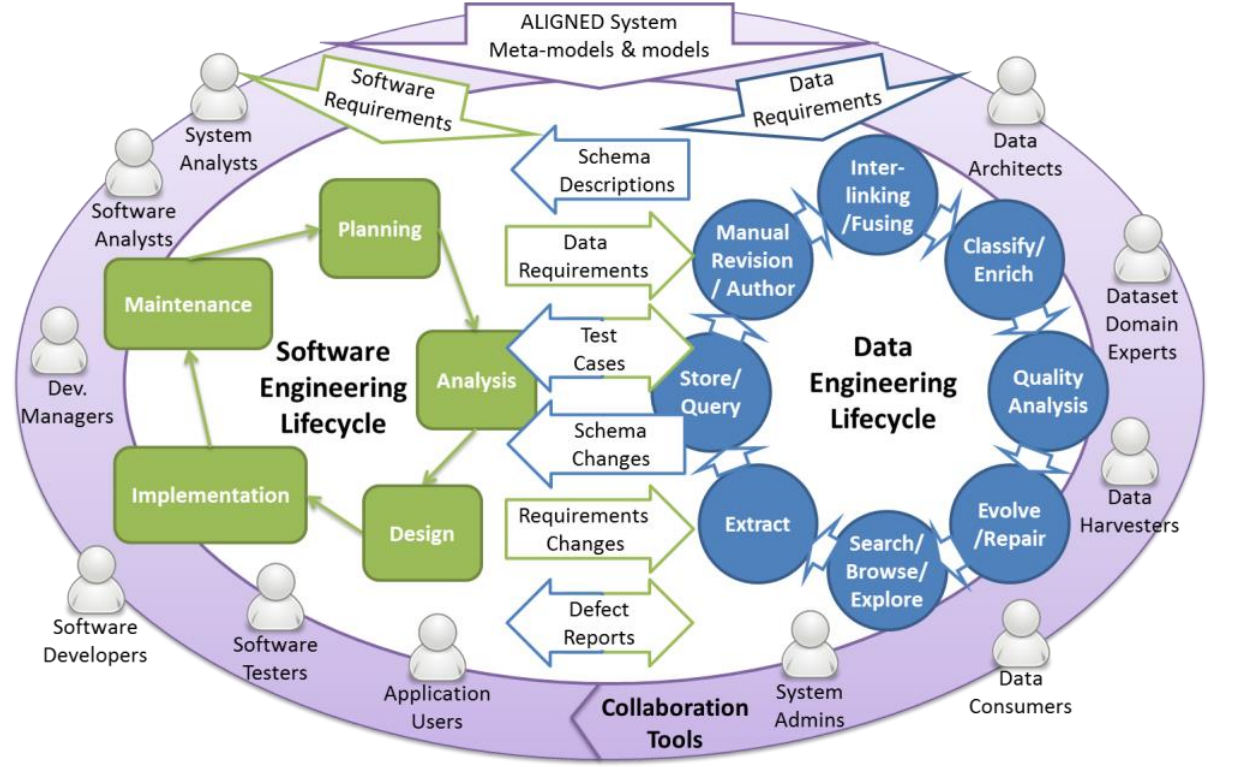
\includegraphics[width=\textwidth]{images/AlignedCircles.png}
  \caption{ALIGNED Software and Data Engineering Processes}
  \label{fig:aligned}
\end{figure}
\todo{add a last sentence?}

\section{Structure}
\label{sec:structure}
This work is a comprehensive introduction to \dataid, with a particular focus on the \core ontology, at the heart of the \ecosystem. It is largely based on four publications:
\begin{enumerate}
\item Martin Brümmer, Ciro Baron, Ivan Ermilov, Markus Freudenberg, Dimitris Kontokostas and Sebastian Hellmann  "DataID: Towards Semantically Rich Metadata for
Complex Datasets". In: Proceedings of the 10th International Conference on
Semantic Systems. SEM ’14. Leipzig, Germany: ACM, 2014, pp. 84–91. \cite{dataID2014}
An introduction to the first version of \dataid.
\item Monika Solanki, Bojan Bozic, Markus Freudenberg, Dimitris Kontokostas, Christian Dirschl and Rob Brennan "Enabling Combined Software and Data Engineering
at Web-Scale: The ALIGNED Suite of Ontologies". In: The Semantic Web -
ISWC 2016 - 15th International Semantic Web Conference, Kobe, Japan, October
17-21, 2016, Proceedings, Part II. 2016, pp. 195–203. \cite{SolankiBFKDB16}: An overview of the landscape of ontologies developed by the ALIGNED project.
\item Markus Freudenberg, Martin Br{\"u}mmer, Jessika R{\"u}cknagel, Robert Ulrich, Thomas Eckart, Dimitris Kontokostas and Sebastian Hellmann "The Metadata Ecosystem of DataID". In: Metadata and Semantics Research: 10th International Conference, MTSR 2016, Göttingen, Germany, November 22-25, 2016, Proceedings. Ed. by Emmanouel
Garoufallou et al. Cham: Springer International Publishing, 2016, pp. 317–332. I S B N : 978-3-319-49157-8. \cite{Freudenberg2016}: An introduction the \ecosystem
\item DataID core Ontology (2017): A W3C member submission of the University of Leipzig, under review by the W3C at the time of writing, authored by Martin Brümmer and me.\todo{add ref}
\end{enumerate}

After a look at related work (chapter 3) on the subject of dataset metadata, I will present the \ecosystem in chapter 4, to introduce the guiding principles of this work. Chapter 5 describes the \core ontology in detail, containing a running example of a \todo{what is this?} DBpedia language edition. 
Chapter 6 provides a best practice about publishing data on the Web with \dataid, followed by an application of those practice to a real example on how to solve complex metadata challenges with the \ecosystem, by looking at Data Management Plans (chapter 7).
Chapter 8 provides mappings between \dataid and multiple \cmd profiles of the Component MetaData Infrastructure (\cmdi). I will evaluate \dataid in chapter 9 and discuss its development and future work in chapter 10. 
%In a previous version of DataID\cite{dataID2014} we already provided a solution for an accessible, compatible and granular best-practice of dataset descriptions for Linked Open Data (LOD).

%We want to build on this foundation, presenting improvements in regard to \provenance, \licensing and \access. In particular, we want to address the aspects \extensibility and \interoperability of dataset metadata, demonstrating the universal applicability of DataID in any domain or scenario.
%As a proof of concept for its \extensibility we will show how to provide extensive metadata for Data Management Plans (\dmp) of research projects (cf. \Cref{dmps}) by extending the DataID model with properties specific to this scenario.
%The \interoperability with other metadata models is exemplified by the mapping of common \cmdi (CLARIN) profiles to DataID in \Cref{cmdi}.


\chapter{Foundations}
\label{chap:foundations}

\section{Data}
\label{sec:data}
Data is an almost intangible term. It is highly ambiguous and touches many fields of interest, stretching from philosophy to digital signal processing. Even in the context of Information Science, Data has multiple possible definitions. Here are some of them:

\begin{quote}
"Data is a symbol set that is quantified and/or qualified." (Prof. Aldo de Albuquerque Barreto, Brazilian Institute for Information in Science
and Technology, Brazil \cite{Zins2007})
\end{quote}

\begin{quote}
"Data are sensory stimuli that we perceive through our senses." (Prof. Shifra Baruchson–Arbib, Bar Ilan University, Israel \cite{Zins2007})
\end{quote}

\begin{quote}
"By data, we mean known facts that can be recorded and that have implicit meaning." (Prof. Shamkant Navathe, College of Computing at the Georgia Institute of Technology, USA \cite{elmasri06db})
\end{quote}

\begin{quote}
"Etymologically, data [...] 
is the plural of datum, a noun formed from the
past participle of the Latin verb dare–to give. Originally,
data were things that were given (accepted as "true"). A data
element, d, is the smallest thing which can be recognized as
a discrete element of that class of things named by a specific
attribute, for a given unit of measure with a given precision
of measurement." (Prof. Charles H. Davis, Indiana University, USA \cite{Zins2007})
\end{quote}

\begin{quote}
"Data are the basic individual items of numeric or other information,
garnered through observation; but in themselves,
without context, they are devoid of information."
(Dr. Quentin L. Burrell, Isle of Man International Business School, Isle of Man \cite{Zins2007})
\end{quote}

Information and Data seem to be closely linked and are often used interchangeably, yet they are not the same thing:

%Data has become the crude oil of the information age, to the extent where we can no longer speak of ours as an "information society". The call of new, vast, untapped data lakes representing limitless potential value has driven businesses, researchers and governments into an frenzied activities to produce, collect and spy out new data. The "data society" seems to be the appropriate branding of these new surroundings.

%\blockquote[\cite{ventre2016information}]{
%"Data represent the raw material, the resource , which feeds and flows through our systems, the global network of communications between individuals, between machines ans systems. Companies produce data, as do individual citizens, institutions, and the technical systems themselves; data have acquired a market value, a strategic value, so people steal them and resell them [...]."
%}
%Technical and social challenges arising from the ever-increasing flow of Data are plentiful and diverse (as touched on in the introduction of this work). 


\begin{quote}
"Datum is every thing or every unit that could increase the
human knowledge or could allow to enlarge our field of scientific,
theoretical or practical knowledge, and that can be
recorded, on whichever support, or orally handed. Data can
arouse information and knowledge in our mind." (Prof. Maria Teresa Biagetti, University of Rome 1, Italy; based on C. S. Peirce, 1931,
1958 \cite{Zins2007})
\end{quote}

I will take a broader look at the term Data, delineating it from the concepts of Information and Knowledge.

\subsection{Data, Information, Knowledge}
\label{sec:kids}

\textit{Data} is the result of the application of syntactical rules against a set (sequence, string etc.) of signs or signals, out of which a message between a sender and recipient is constructed \cite{bodendorf2003daten}. Additional schematics might apply, adding structural data. \textit{Information} can be gleaned from data if one can find meaning in it. The result of this semantic expansion (or interpretation) of \textit{Data} can be weighted by its novelty value or exceptionalness in the context of existing information, using Shannon's entropy \cite{shannon48}. \textit{Data} becomes tokens of perceptions, or more commonly used in Information Science: instances of concepts, capable of changing the understanding of a context for the recipient of the original message. Linking \textit{Information} in a context to determine their interrelations and inferring additional information under the presumption of an intellectual goal, are the processes (\textit{Pragmatics}) turning \textit{Information} into \textit{Knowledge}.

\begin{figure}[t]
\centering
  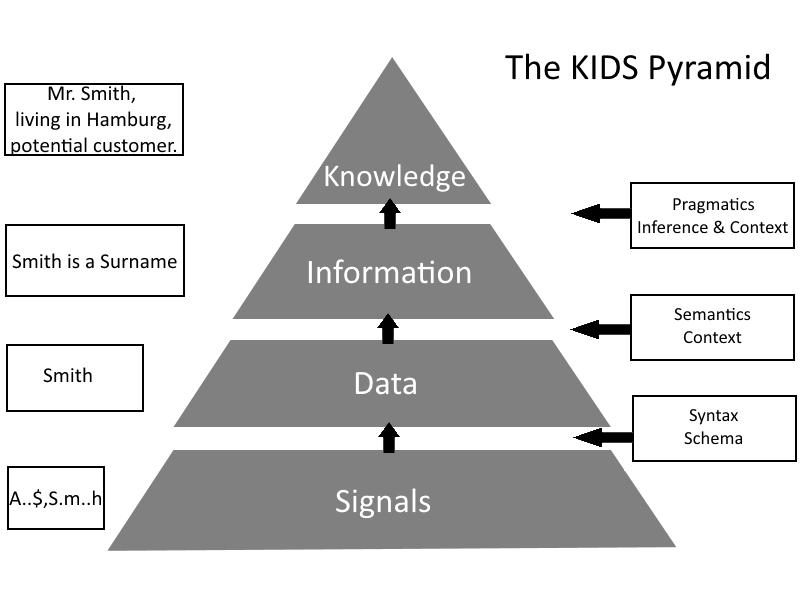
\includegraphics[width=\textwidth]{images/kidsPyramid.png}
  \caption{The KIDS Pyramid \cite{bodendorf2003daten}}
  \label{fig:kids}
\end{figure}

The pyramidal structure depicted (\cref{fig:kids}) is often crowned by an additional field called "Wisdom" \cite{Rowley2007}. Wisdom could be described as a form of evaluated \textit{Knowledge} or understanding, as the pinnacle of human endeavour or enlightenment. But in the era of fake news, pathological mistrust and truthiness\footnoteurl{https://en.wikipedia.org/wiki/Truthiness}, this last step does not seem to follow naturally.

Many authors describe this hierarchy or derivations of it. The following common aspects are presented throughout this literature \cite{Rowley2007}: \todo{check if we need quotation here}

\begin{itemize}
\item the key elements are data, information and knowledge,
\item these key elements are virtually always arranged in the same order, some models offer additional stages, such as wisdom, or enlightenment,
\item the higher elements in the hierarchy can be explained in terms of the lower elements by identifying an appropriate transformation process,
\item the implicit challenge is to understand and explain how data is transformed into information and information is transformed into knowledge.
\end{itemize}

\subsection{Digital Data}
\label{sec:digital}
Digital data is represented using the binary number system of ones (1) and zeros (0). Typically, these are combined into eight of their kind - named Byte. Bytes are used to identify characters of a given alphabet, which, in turn, provide the building stones for any operation, program or data point (datum).

In general, the term Digital Data is used to describes a collection of bytes, representing a digital mapping of an analogue counterpart (e.g. sound waves), or characters of an alphabet understood by humans or programs.

Digital Data is often categorized in structured and unstructured data. Unstructured data does not follow any predefined model and has to be interpreted by the recipient (reader) by its own merit (usually free text). Structured data is strictly adherent to a given data model, facilitating its interpretation by machines and humans alike (such as [please insert]). 
%Semi structured data allows for unstructured parts in a structured context (e.g. XML [needs link]).

\subsection{Dataset}
\label{sec:dataset}

A dataset\footnote{or 'data set', though this spelling seems to be replaced more and more} is a bundle of data, which have at least one common dimension of distinction. For example, a music album of an artist can be viewed as a dataset, where a single song represents a unit of data. Multiple songs are collected in an album with the common feature (among others) - the artist. Most commonly a dataset corresponds to a collection of structured (digital) data in a single location (e.g. a database table, XML document etc.).

Datasets can manifest in different formats (e.g. in different file types). Therefore, the distinction between dataset as a container for collecting data points of similar content or structure, and its final manifestation on a file system, is advisable.


\subsection{Metadata}
\label{sec:metadata}

The National Information Standards Organization\footnoteurl{http://www.niso.org/home/} (NISO), a United States non-profit standards organisation, published a paper in 2004, defining metadata in a widely adopted manner:

\begin{quote}
"Metadata is structured information
that describes, explains,
locates, or otherwise makes it
easier to retrieve, use, or manage
an information resource. Metadata
is often called data about data or
information about information." \cite{NISO2004}
\end{quote}

Metadata does not contributes additional content to the original message, but it can ease its transmission, procession and understanding.
The meaning of the term metadata and for what kind of data it applies is different, depending on context, disciplines and communities.
For example, library catalogue information about a certain book might be understood as metadata in regard to the book itself, while in the context of a Library Management System this type of metadata is considered data.

Specialized types of metadata can be broadly separated into three types \cite{NISO2004}:

\begin{itemize}
\item \textbf{Descriptive metadata} describes a resource for purposes such as discovery and identification. It can include elements such as title, abstract, author, and keywords. 
\item \textbf{Structural metadata} indicates how compound objects are put together, for example, how pages are ordered to form chapters.
\item \textbf{Administrative metadata} provides information to help manage a resource, such as when and how it was created, file type and other technical information, and who can access it. Subsets of administrative metadata include:
\begin{itemize}
\item \textbf{Rights management metadata}, which deals with intellectual property rights and licenses.
\item \textbf{Preservation metadata}, which contains information needed to archive and preserve a resource.
\end{itemize}
\end{itemize}

A metadata record conforms to a given schema, since the use of unstructured data to qualify a different data resource is an exercise in futility. Various metadata schemata or ontologies are available, often describing similar types of data. The most commonly used metadata vocabulary is Dublin Core\footnoteurl{http://dublincore.org/documents/dces/} (DC) by the Dublin Core Metadata Initiative (DCMI):

\begin{quote}
"The original objective of the
Dublin Core was to define a set of
elements that could be used by
authors to describe their own Web
resources. [...] the goal was to define a
few elements and some simple
rules that could be applied by
noncatalogers [sic]." \cite{NISO2004}
\end{quote}

The following example illustrates the use of Dublin Core attributes (e.g. \prop{dc:description}) to describe a publication released as an PDF file:

\begin{lstlisting}[language=ttl, captionpos=b, caption=Dublin Core example, label=lst:dcex,linewidth=\columnwidth,breaklines=true]
dc:title="Metadata Demystified"
dc:creator="Brand, Amy"
dc:creator="Daly, Frank"
dc:creator="Meyers, Barbara"
dc:subject="metadata"
dc:description="Presents an overview of metadata conventions."
dc:publisher="NISO Press"
dc:publisher="The Sheridan Press"
dc:date="2003-07-01"
dc:type="Text"
dc:format="application/pdf"
dc:identifier="http://www.niso.org/standards/resources/metadata.pdf"
dc:language="en"
\end{lstlisting}

All Dublin Core attributes are optional, repeatable (non-functional) and present without order. Controlled vocabularies\footnote{a set of predefined values, controlled by an institution or a body of experts} are recommended to be used in connection with some fields (such as \prop{dc:subject}). Since its introduction in 1995, the initial list of 15 attributes has been revised and extended, forming the so called DCMI Metadata Terms\footnoteurl{http://dublincore.org/documents/dcmi-terms/} (DCT). The very general character of this vocabulary provides a useful foundation for more complex schemata reusing DC (for example \dcat).

Metadata can describe any resource in any state or aggregation (single resource, collections, a part of a resource). Any resources, at any abstraction level of a domain model can be substantiated with metadata.
The International Federation of Library Associations and Institutions\footnoteurl{http://www.ifla.org} (IFLA) defined the "Functional Requirements for Bibliographic Records" \cite{IFLA-Functional-1998}, a conceptual model for retrieval and access in online library catalogues and bibliographic databases: \textbf{Item} is an exemplar of a \textbf{Manifestation}, which embodies an \textbf{Expression}, realising a \textbf{Work} of an author.

For example, a metadata record could describe a report, a particular edition of the report, or a specific copy of that edition of the report. \todo{is this a quote?}

Metadata can be embedded in the described digital object, alongside the object (e.g. in the same directory) or stored separately. HTML documents often keep metadata in the HTML header or completely emerged in the document (see RDFa \cite{McCarronRDFaW3C2015}). While a close coupling between data and metadata is useful when updating them together, a separate approach often simplifies the management of large numbers of records.

The advantages of reliable metadata for digital objects are manifold. These are the more poignant attributions of metadata:

\begin{description}
\item [Resource Discovery:] Metadata is the foremost source of information which aids agents (persons, software etc.) to discover wanted data.
\item [Organising Electronic Resources:] Entities (e.g. books in a library) are organised in catalogues with the help of their digital metadata records.
\item [Interoperability:] The interoperability of two digital resources can be determined by comparing their metadata entries, on a syntactical as well as on a semantic level.
\item [Digital Identification:] Digital identifiers (such as URIs \cref{sec:semweb}) are stored with metadata records.
\item [Provenance:] An extensive record on provenance is a key for trustworthiness, detailing facts like source data, responsible agents or origin activities.
\item [Quality:] The quality of a data source is also established by the quality of its metadata.
\item [Reusability:] Increasing discoverability, interoperability, provenance and quality are instrumental requirements for increasing reusability. 
\item [Preservation:] "Metadata is key to ensuring that resources will survive and continue to be accessible into the future." \cite{NISO2004}
\end{description}

In the chain of processes transforming Signals, Data, Information into Knowledge (\cref{sec:kids}), metadata can help with all transformation steps:

\begin{itemize}
\item To provide information about schemata to which a set of structured data adheres or the syntax description needed to understand the signs transmitted.
\item To advance the interpretation of data by providing context information (e.g. geographical or temporal).
\item To point out related (web-) resources to broaden the context of an information (e.g. links to similar datasets or related web site).
\end{itemize}

%Metadata for datasets should provide for all of these benefits and reflect the FAIR principles (see next section \ref{sec:fair}). Specifically, dataset metadata should feature:

%\begin{itemize}
%\item machine readable resources (no free text if possible);
%\item well defined abstraction levels (e.g. dataset, dataset catalogue etc.);
%\item a detailed portrayal of internal hierarchies (sub-datsets);
%\item exhaustive descriptions for data access (e.g. access procedures, capacity limitations etc.)
%\item detailed license and rights portrayal
%\item capability for an extensive description of provenance information (involved agents, source datasets etc.)
%\end{itemize}

%These demands on dataset metadata are not particularly unique features, but are of enormous importance to automatically process and evaluate metadata and the described data alike.
%\pagebreak
\subsection{The FAIR Data Principles}
\label{sec:fair}

In 2014, a workshop in Leiden, Netherlands, was held, named "Jointly Designing a Data Fairport". A wide group of academics and representatives of companies and other organisations concluded the workshop by drafting a concise and measureable set of principles to overcome common obstacles, impeding data discovery and reuse of (scientific) data.

The \textbf{FAIR} Guiding Principles \cite{fair2016}

\begin{enumerate}
\item[\textbf{F}] \textbf{To be Findable:}
\begin{enumerate}[1]
\item (meta)data are assigned a globally unique and persistent identifier
\item data are described with rich metadata (defined by R1 below)
\item metadata clearly and explicitly include the identifier of the data it describes
\item (meta)data are registered or indexed in a searchable resource
\end{enumerate}
\item[\textbf{A}] \textbf{To be Accessible:}
\begin{enumerate}[1]
\item (meta)data are retrievable by their identifier using a standardized communications protocol
\begin{enumerate}
\item the protocol is open, free, and universally implementable
\item the protocol allows for an authentication and authorization procedure, where necessary
\end{enumerate}
\item metadata are accessible, even when the data are no longer available
\end{enumerate}
\item[\textbf{I}] \textbf{To be Interoperable:}
\begin{enumerate}[1]
\item (meta)data use a formal, accessible, shared, and broadly applicable language for knowledge representation.
\item (meta)data use vocabularies that follow FAIR principles
\item (meta)data include qualified references to other (meta)data
\end{enumerate}
\item[\textbf{R}] \textbf{To be Reusable:}
\begin{enumerate}[1]
\item (meta)data are richly described with a plurality of relevant attributes
\item (meta)data are released with a clear and accessible data usage license
\item (meta)data are associated with detailed provenance
\item (meta)data meet domain-relevant community standards
\end{enumerate}
\end{enumerate}

\pagebreak
\section{Semantic Web}
\label{sec:semweb}

I presented our common understanding of how data can herald information and knowledge in \cref{sec:kids}. I refrained from specifying which step or state might be restricted to humans or machines. None of those restrictions would probably be correct. While I don't want to elaborate on the question of: "Can machines have Knowledge?", I do state that machines can glean information from data. To interpret a message and derive meaning is not limited to the human mind. All what is needed is context and an understanding of the concepts a domain is constituted of (semantics).

In 2001, Tim Berners-Lee, Hendler, and Lassila layed out their expectation of how the World Wide Web will eventually extend to become a Semantic Web \cite{Semweb1}. The simple extension of web resources with structured, well defined data (or metadata) would give meaning to resources, previously only decipherable by humans. To identify these data resources uniquely by Universal Resource Identifiers (URI) and provide links to other resources, would be the first steps in the direction towards a "web of data that can be processed directly and indirectly by machines". \todo{quote?}

\begin{quote}
"The Semantic Web is not a separate Web but an extension of the current one, in which information is given well-defined meaning. better enabling
computers and people to work in cooperation." \cite{Semweb1}
\end{quote}

Tim Berners-Lee is the director of the World Wide Web Consortium\footnoteurl{https://w3.org} (W3C), which is responsible\todo{rewrite} for the development of standards for the World Wide Web, and by extension for the Semantic Web. At its core, the Semantic Web is defined by a collection of standards, which are \textit{Recommendations} by the W3C. "Semantic Web technologies enable people to create data stores on the Web, build vocabularies, and write rules for handling data." \footnoteurl{https://w3.org/standards/semanticweb/}.

\subsection{Resource Description Framework (RDF)}
\label{sec:rdf}

This foundational technology of the Semantic Web and recommendation of the W3C \cite{RDF11} is used to describe any resource, using URIs as identifiers. Resources are defined by set of characteristics which are expressed as attributes or relations to other resources. Statements in the form of "subject, predicate, object" (named "triples") are used to convey such characteristics. The resource described is uniquely identified by the URI of the subject. The object corresponds to the content or reference of the statement. Literals (strings) are used to serialize content (or values), URIs of resources provide the target of a reference. The predicate is the semantic link between the subject and the object and defines the meaning of this statement.
This simple linguistic construct makes RDF data understandable for humans and machines alike:

\begin{lstlisting}[language=ttl, label=lst:triple,linewidth=\columnwidth,breaklines=true]
<http://dbpedia.org> publisher "DBpedia Association".
\end{lstlisting}

This triple describes the resource http://dbpedia.org (identified by the URI of the subject). Its object is the literal "DBpedia Association" connected to the subject with the predicate: publisher. Without the predicate, no meaning could be ascribed to the datum "DBpedia Association", as the type of relation between subject and object would be unknown. Thus, the predicate is what lends meaning to a statement.

The same information about the publisher of a website could be expressed differently in RDF data model. Since "DBpedia Association" represents an organisation, it could be introduced and described as an instance of a concept named "Organisation". This instance is capable of providing multiple attributes, not only its name:

\begin{lstlisting}[language=ttl, label=lst:graph,linewidth=\columnwidth,breaklines=true]
<http://dbpedia.org> publisher <http://dbpedia.org/DBpediaAssociation>.
<http://dbpedia.org/DBpediaAssociation> type "Organisation".
<http://dbpedia.org/DBpediaAssociation> name "DBpedia Association".
<http://dbpedia.org/DBpediaAssociation> headquarter "Leipzig". 
\end{lstlisting}

It is obvious that the instantiation of the objects "Organisation" and "Leipzig" would bear the same benefits. 
By extending this list of statements, describing additional resources and their characteristics, a directed graph is constructed. The data of this graph is highly interlinked and has the ability to relate to resource descriptions outside this graph as well. A URI identifies a resource in the world without ambiguity (when carefully constructed based on existing domain names). This allows linking of data objects without regard to resource locations (datasets, service endpoints etc.) and institutions, creating, what is called, "Linked Data" (\cref{sec:ld}).

While labels like "publisher" have meaning for humans, they are ambiguous and could be misinterpreted. 
Especially machines cannot resolve this ambiguity and could not infer meaning from such statements. 
To address this issue, predicates are also identified by URIs that can be looked up for further information.
Predicates are called properties in the RDF data model.

\begin{lstlisting}[language=ttl, label=lst:graph,linewidth=\columnwidth,breaklines=true]
<http://dbpedia.org> <http://purl.org/dc/terms/publisher> <http://dbpedia.org/DBpediaAssociation>.
<http://dbpedia.org/DBpediaAssociation> <http://purl.org/dc/terms/name> "DBpedia Association".
\end{lstlisting}

Sets of properties can be defined and documented by institutions, like DCMI (\cref{sec:metadata}). They can then be reused by others, increasing interoperability and reusability. These sets of properties together with associated concepts and annotations are called ontologies.


\subsection{Web Ontology Language (OWL)}
\label{sec:owl}

The Web Ontology Language is a W3C recommended standard \cite{OWL2} based on the RDF data model, which could be summarized as an ontology for defining ontologies. An ontology is a set of concepts, properties and logical axioms, with which to model a domain of knowledge or discourse. This conceptualization of a given domain or idea, allows for a formal representation with RDF as well as its automatic interpretation by machines.

Concepts are classes under which all objects of a domain can be classified, dividing up the domain in abstract objects. Properties provide meaning for the links to instances of concepts or literal objects (values), which, in turn, lends meaning to the concepts themselves. Additionally, subclass relations and restrictions on properties (e.g. domain and range definitions) help to specify more complex relations of a domain. This semantic layer between the domain knowledge on one side and its representation in RDF on the other is free of restrictions imposed by underlying technologies, distinguishing it from other data models (e.g. database schemata). A wide range of ontologies are available for any type of domain. Upper ontologies are general use vocabularies (such as Dublin Core \cref{sec:metadata}) which can be reused together with other ontologies. High reusability is another difference to many other domain description languages. 

Multiple langauge profiles are available \cite{OWLPROFILES}, introducing different logical regimes to OWL, such as Description Logic (OWL-DL) or based on Rule Languages (OWL2-RL). Profiles allow for reasoning over RDF data, adhering to ontologies under such regimes. The profile OWL Full is an extension of the RDF Schema (RDFS \cite{RDFS11}), which provides basic elements for the description of ontologies (allowing for class hierarchies and basic relations).

Description Logic is a fragment of first-order predicate logic \cite{Barwise1977} and a formalism for representing knowledge. OWL is heavily influenced by Description Logic (projects like DAML+OIL \cite{HPMW07}) in order to achieve a beneficial trade-off between language expressiveness and computational complexity of reasoning.


\subsection{Linked Data}
\label{sec:ld}
Linked Data is the idea of how data is freed from an islands of unconnected data, so it can be used and referenced all over the world referencing simply their URIs. Links between data objects from different sources are not bound to restrictions, authorisation procedures, licensing or any technical obstacles, they simply state that: "There is a data object (published in a well defined manner - e.g. RDF) which is related and it is identifiable on the Web with this URI". Machines and humans can follow up these links and explore the "Web of Data", expanding the contextual information.\todo{needs link}

\begin{quote}
"Technically, Linked Data refers to data published on the Web in such a way that it is
machine-readable, its meaning is explicitly defined, it is linked to other external data sets,
and can in turn be linked to from external data sets." \cite{bizer_linked_2009}
\end{quote}

Additionally, a set of best practices were contrived by Tim Berners-Lee to identify the necessary steps needed to publish and link structured data on the Web, since "a surprising amount of data isn't linked in 2006, because of problems with one or more of the steps" \cite{5starData}.

\begin{enumerate}
\item Use URIs as names for things.
\item Use HTTP URIs so that people can look up those names.
\item When someone looks up a URI, provide useful information, using the standards (RDF, SPARQL).
\item Include links to other URIs. so that they can discover more things.
\end{enumerate}

Linked Data extends the demands of RDF as a data model by specifying HTTP as the access
layer of choice and requiring the openness of the resource to be regarded of high quality. \todo{quote}
The result is a Web of Data, a machine-readable, semantic network of structured data, 
opposed to the HTML based web of documents (from humans, for humans).

\chapter{Related Work}
\label{chap:relatedwork}

\section{Dataset vocabularies}
\label{sec:dv}
This section is dedicated to dataset metadata vocabularies and application profiles \footnote{a set of metadata elements defined for a particular application or other limited purpose, often based on a broader schema (like an ontology)}, to compare them and list their (dis-) advantages.

Based on the FAIR Data Principles (\cref{sec:fair}) and the list of important aspects of dataset metadata (\cref{sec:motivation}), I contrived the following list of aspects, against which I want to evaluate each vocabulary.

\begin{enumerate}[A]
\item \textbf{The vocabulary encourages the use of richly described and machine-readable resources.} 
Concepts are defined as exhaustive as necessary to describe all relevant aspects, avoiding free text properties in general. For example, replacing a literal with a well structured instance of \prop{foaf:Agent}. 
\item \textbf{The vocabulary assigns globally unique URIs to metadata resources.} Demanding URIs as identifiers, independent of the chosen data representation (even for non RDF or XML metadata).
\item \textbf{The vocabulary can describe data access related properties and restrictions, enabling access for humans and machines alike.} Sufficient effort has been made to describe this important aspect in detail, considering all possible formats of a dataset.
\item \textbf{The vocabulary can portray provenance information extensively.} Dataset provenance can be described extensively, including other datasets (e.g. sources), activities (e.g. data generation activities) and agents (e.g. publisher) as well as inter-relational properties between these concepts.
\item \textbf{The vocabulary provides for detailed descriptions of rights and licenses.} Machine readable licenses are of utmost importance.
\item \textbf{The vocabulary provides properties to cite identifiers of the data described.} The possibility to reference the data described directly (by identifier) in the metadata is available.
\item \textbf{The vocabulary provides for qualified references between resources.} Relations between instances of dataset metadata can be qualified by roles (specifying the type of relations), time and other restrictions.
\item \textbf{The vocabulary is easy to extend, to fit any given use case.} The vocabulary is general enough to fit any use case, it can easily be extended and no unnecessary restrictions, like restrictive cardinalities, are in place.
\item \textbf{The vocabulary is unambiguous and easy to map to other metadata vocabularies.} The vocabulary is general enough to be able to match other metadata formats. Properties are defined clearly without overlapping the purpose of others (so users know which property to use).
\item \textbf{The vocabulary offers additional properties to aid dissemination and discovery.} Extra properties are in place to provide keywords, genres, taxonomy concepts and general statements explaining the use of a dataset.
\end{enumerate}

I will assign one of the following ratings to every item: \textbf{(2)} The requirement is supported in full. \textbf{(1)} The requirement is partially met. \textbf{(0)} The vocabulary does not support this requirement. 
While this list is helpful for evaluation and comparison purposes, the quality of a dataset vocabulary is also dependent on the intended domain of use and other factors, which I will mention as well.

\subsection{The Data Catalog Vocabulary (DCAT)}
\label{sec:dcat}
In \cite{MaaliCP10} the authors introduce a standardised interchange format for machine-readable representations of government data catalogues. The Data Catalog Vocabulary (\dcat) is a W3C recommendation \cite{ddcat} and serves as a foundation for many available dataset vocabularies and application profiles.
Vocabulary terms for \dcat are inferred from the survey on seven data catalogues from Europe, US, New Zealand and Australia.

\begin{quote}
"By using \dcat to describe datasets in data catalogs, publishers increase discoverability and enable applications easily to consume metadata from multiple catalogs. It further enables decentralized publishing of catalogs and facilitates federated dataset search across sites." \cite{ddcat}
\end{quote}

\dcat defines three levels of abstraction, based on the following distinctions: A dataset describes a "collection of data, published or curated by a single agent, and available for access or download in one or more formats"\cite{ddcat}, and represents the commonalities and varieties of the data held within (the 'idea' or intellectual content of that dataset). A Dataset is part of a data catalogue, representing multiple datasets (e.g. of an organisation). Datasets manifest themselves (are available) in different forms (such as files, service endpoints, feeds etc.), expressed with the class \prop{dcat:Distribution}. A dataset might be available for download at two different locations on the Web and available to be queried through an API endpoint. This scenario can be described by using three different \prop{dcat:Distribution} instances.

\begin{figure}[!htbp]
\centering
  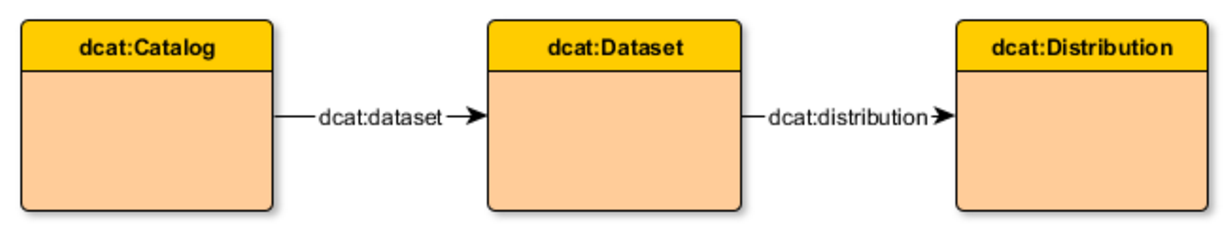
\includegraphics[width=\textwidth]{images/DcatIdea.png}
  \caption{The basic idea of \dcat}
  \label{fig:dcat}
\end{figure}

This basic idea of differentiating between catalogue, dataset and distribution, has prevailed throughout the metadata domain for digital resources (not only datasets), and has become an quasi-requirement for metadata representations of web resources\footnoteurl{https://www.w3.org/TR/dwbp/#context}. In fact, the general approach the authors of \dcat took, makes it possible to describe any digital object. This is a highly desirable feature, supporting \extensibility and \interoperability of the vocabulary.

As stated before (\cref{sec:motivation}), a downside to this approach is the possible unspecificity of resources, especially in regard to machine-readability, where uncertainty about formats is problematic.

\textbf{Insufficient provenance information:}
\begin{itemize}
\item \dcat expresses provenance in a limited way using a few basic properties such as
\prop{dct:source} or \prop{dct:creator}, which can not be further qualified.
\item No possibility to specify activities involved in the creation of datasets.
\item There is no support or incentive to describe source datasets, related publications or conversion activities of transformations responsible for the dataset. This lack is crucial, especially in a scientific contexts, as it omits the processes necessary to replicate a specific dataset.
\item Insufficient portrayal of context information (e.g. licenses, geography etc.)
\end{itemize}

\textbf{Missing relations between Datasets:}
\begin{itemize}
\item in general: Referencing related datasets is only possible on a very generic scale (e.g. \prop{dct:relation}).
\item hierarchical: No inherent portrayal of dataset hierarchies is possible.
\item evolutionary: No versioning pointers between dataset representations.
\end{itemize}

\textbf{Relations to agents are too cursory:}
\begin{itemize}
\item A very restricted number of properties pointing out agents, without any further qualification (e.g. \prop{dct:publisher}, \prop{dcat:contactPoint}), other related entities, like software, projects, funding etc., are neglected all together.
\item No agent role concept to define new relations.
\end{itemize}

\textbf{Technical description of distributions is lacking, restricting the accessibility of the data:}
\begin{itemize}
\item Only superficial attributes for describing the technical characteristics of a distribution are available.
\item No access information are available, such as access restrictions or service description, needed to describe service endpoints.
\item No specificity when describing serialisation or media type of a distribution (e.g. file format).
\end{itemize}

\textbf{General lack of specificity, inviting non-machine-readable expressions of resources:}
\begin{itemize}
\item Insufficient specificity of property ranges (e.g.: \prop{dct:license}, \prop{dct:temporal}, \prop{dct:spatial}, \prop{dct:language}, \prop{dcat:mediaType}), thereby neglecting exactness of relevant metadata resources, such as licenses.
\item A lack of referential and functional integrity due to missing role-based qualifications of properties (such as \prop{dct:maintainer}) \cite{jefferyCerifW3C2016}.
\end{itemize}

While this seems to be an extensive list of shortcomings, most of the points listed above are due to the general approach of \dcat. The list merely indicates that portraying dataset metadata with \dcat alone, might not be sufficient for most domains and use cases.

In turn, extending \dcat as upper ontology provides a sufficient basis for any metadata descriptions, without regard to domain or use case. Adopting not only its basic ideas, but the aspects of easy \extensibility and \interoperability, should prove beneficial. Addressing the issues with \provenance, \licensing and \access as well as domain specific demands for metadata is the central task I set out to complete.

\todo{The evaluation table is reused in the eval section. The numbers within have to be revisited...}
\begin{table}[!htbp]
    \centering
    \begin{tabular}{|l|l|l|l|l|l|l|l|l|l|l|l|}
        \hline
        Requirement & A & B & C & D & E & F & G & H & I & J & Sum \\
        \hline
        Evaluation of \dcat & 2 & 2 & 0 & 0 & 0 & 1 & 0 & 2 & 2 & 2 & 11 \\
        \hline
    \end{tabular}
    \label{tab:evaldcat}
\end{table}

\subsection{Vocabulary of Interlinked Datasets (VoID)}
\label{sec:void}

The Vocabulary of Interlinked Datasets (\void) \cite{Alexander09describinglinked} is widely accepted and used within the Semantic Web community, for instance in projects such as: OpenLink Virtuoso\footnoteurl{http://virtuoso.openlinksw.com/} , LODStats\footnoteurl{http://stats.lod2.eu/} , World Bank\footnoteurl{http://worldbank.270a.info/} and others. \void can be used to express general metadata, access metadata, structural metadata and links between Linked Data datasets. Tools to create \void metadata are described in \cite{DBLP:BohmLN11} where authors also presents techniques of reduction in order to create descriptions for Web-scale datasets. In the same paper the importance of \void is well established but there is still a lack of important metadata which is not described, for example license and provenance. For simple datasets \void performs well, which is supported by the fact of wide acceptance of the vocabulary. 
However, in a case of complex datasets \void is not expressive enough. In particular, access metadata includes the \prop{void:dataDump} property, which points to the data files of the particular dataset. This property should link directly to dump files as described in W3C Interest Group Note: Describing Linked Datasets with the \void Vocabulary\footnoteurl{http://www.w3.org/TR/void/}. Thus, additional semantic information about the data files and the structure of the dataset can not be expressed using \void. Moreover, \void does not provide a distribution concept depriving the vocabulary of an important level of abstraction. Yet, this ontology is useful especially for Linked Data datasets, offering many useful statistical properties (such as \prop{void:triples}) and the very handy concept of \prop{void:LinkSet} describing the particular relation between datasets, where one holds links to instances of the other.

\begin{table}[!htbp]
    \centering
    \begin{tabular}{|l|l|l|l|l|l|l|l|l|l|l|l|}
        \hline
        Requirement & A & B & C & D & E & F & G & H & I & J & Sum \\
        \hline
        Evaluation of \void & 2 & 2 & 1 & 1 & 0 & 0 & 1 & 1 & 1 & 1 & 10 \\
        \hline
    \end{tabular}
    \label{tab:evalvoid}
\end{table}

\subsection{Comprehensive Kerbal Archive Network (CKAN)}
\label{sec:ckan}

Metadata models vary and most of them do not offer enough granularity to sufficiently describe complex datasets in a semantically rich way. 
For example, \ckan{}\footnoteurl{http://ckan.org/} (Comprehensive Knowledge Archive Network), a data management system used widely in (Open) Data Portals (such as datahub.io\footnoteurl{http://datahub.io/}) to provide web representations for datasets, operates on a JSON  based schema\footnoteurl{https://github.com/KSP-CKAN/CKAN/blob/master/CKAN.schema} developed by the Open Knowledge Foundation\footnoteurl{https://okfn.org}.
\ckan allows simple access to a whole range of functions related to the management of datasets (such as search and faceting of data-sources) accessible via a REST interface.
Its metadata schema has some similarities with \dcat: Datasets are collected under organisation objects, which are used as s primitive stand in for catalogues. Datasets have 'Resources' which assume a similar role as a distribution in the \dcat vocabulary. 

Alas, there is no clear definition of the resource-object within \ckan documentation, nor are there any noteworthy restrictions. This has led to a medley of different use cases for this resource, where it assumes the role of a \prop{dcat:Distribution} in one dataset (containing all data of the dataset) and providing different slices of the data in another example \cite{neum-etal-2016w3c}. Furthermore, the extensive use of key-value pairs for additional data led to a shier host of (semi-) structured data, with only marginal agreement on key names between different Data Portals \cite{neum-etal-2016w3c} adding to the general unclarity of this metadata format, complicating the mapping to other vocabularies.

This data model is semantically poor and inadequate for most applications consuming data automatically. I strongly discourage any organisation from adopting the \ckan format for their dataset metadata. Since it is used so frequently in Data Portals, I feel obliged to point out that there are mapping tools for most vocabularies to \ckan (as I provided for DataID in \cite{dataID2014}).

\begin{table}[!htbp]
    \centering
    \begin{tabular}{|l|l|l|l|l|l|l|l|l|l|l|l|}
        \hline
        Requirement & A & B & C & D & E & F & G & H & I & J & Sum \\
        \hline
        Evaluation of \ckan & 2 & 1 & 0 & 0 & 0 & 0 & 0 & 0 & 1 & 1 & 5 \\
        \hline
    \end{tabular}
    \label{tab:evalckan}
\end{table}


\subsection{Metashare}
\label{sec:metashare}
The \metashare ontology\cite{mccrae_2015_OWLmetashare} is the offspring of a prior, XSD\footnote{XML Schema Definition: a W3C recommendation for how to formally describe the elements in an XML document (https://www.w3.org/TR/xmlschema11-1/)} based "metadata schema that allows aspects of [language resources] accounting for their whole lifecycle from their production to their usage to be described"\cite{mccrae_2015_OWLmetashare}.
\metashare differentiates between language resources (basically datasets with a language related purpose - text, audio etc.), technologies (e.g., tools, services) used for their processing and additional entities like reference documents, agents, projects or licenses. This allows for the portrayal of provenance in the domain of Natural Language Processing.
In addition it offers an exemplary way of describing licenses and terms of reuse\footnoteurl{http://www.cosasbuenas.es/static/ms-rights/}. Yet, \metashare is highly specialised for language resources, thus lacking generality and extensibility for other use cases. While not implementing the \dcat vocabulary, \metashare does provide an almost complete mapping to \dcat. Mappings to other ontologies might prove difficult, due to the large size of the vocabulary and the often employed (and ample) controlled vocabularies. The related \metashare XSD schema has been implemented in the \metashare web portal\footnoteurl{http://www.meta-share.org}, providing many NLP related datasets for download.

\begin{table}[!htbp]
    \centering
    \begin{tabular}{|l|l|l|l|l|l|l|l|l|l|l|l|}
        \hline
        Requirement & A & B & C & D & E & F & G & H & I & J & Sum \\
        \hline
        Evaluation of \metashare & 2 & 2 & 1 & 1 & 2 & 0 & 0 & 0 & 1 & 1 & 10 \\
        \hline
    \end{tabular}
    \label{tab:evalmetashare}
\end{table}

\subsection{Asset Description Metadata Schema (ADMS)}
\label{sec:adms}
The Asset Description Metadata Schema\footnoteurl{https://www.w3.org/TR/vocab-adms/} (\adms) is a profile of \dcat, which is specialised to describe "Semantic Assets".
Assets (as subclass of \prop{dcat:Dataset}) are highly reusable metadata (e.g. code lists, XML schemata, taxonomies, vocabularies etc.) expressing the intellectual content of the data, which is represented (in most cases) in relatively small files. 

\adms adopts the \dcat structure and provides a well defined way of versioning between entities. Its specialised nature makes it unsuited for a broader approach of portraying datasets (as intended by the authors), but it can still contribute useful properties to \dcat based vocabularies (e.g. \cref{sec:dcatap}). Since \adms does not impose any restrictions it can be extended to \dcat without any consequences for \dcat based metadata documents. The evaluation below, therefore does not differ from \dcat.

\begin{table}[!htbp]
    \centering
    \begin{tabular}{|l|l|l|l|l|l|l|l|l|l|l|l|}
        \hline
        Requirement & A & B & C & D & E & F & G & H & I & J & Sum \\
        \hline
        Evaluation of \adms & 2 & 2 & 0 & 0 & 0 & 1 & 0 & 2 & 2 & 2 & 11 \\
        \hline
    \end{tabular}
    \label{tab:evaladms}
\end{table}

\subsection{DCAT Application Profile for data portals in Europe (DCAT-AP)}
\label{sec:dcatap}

The DCAT Application Profile for data portals in Europe\footnoteurl{https://joinup.ec.europa.eu/asset/dcat_application_profile/home} (\dcatap) is a specification based on \dcat (extended with \adms properties) for describing public sector datasets in Europe. It was developed by a working group under the auspices of the European Commission. Its basic use case is "to enable cross-data portal search for datasets and to make public sector data better searchable across borders and sectors" \cite{dcatap11}. This can be achieved by the exchange of descriptions of datasets among data portals.

Traits of the resulting profile\footnoteurl{https://joinup.ec.europa.eu/catalogue/distribution/dcat-ap-version-11} (version 1.1) released in October 2015 \cite{dekkersDcatApW3C2016}:

\begin{itemize}
\item It proposes mandatory, recommended or optional classes and properties to be used for a particular
application;
\item It identifies requirements to control vocabularies for this application;
\item It gathers other elements to be considered as priorities or requirements for an application such as
conformance statement, agent roles or cardinalities.
\end{itemize}

\dcatap has been endorsed by the Standards Committee of ISA2\footnoteurl{https://ec.europa.eu/isa/isa2/index_en.htm} in January of 2016\footnoteurl{https://joinup.ec.europa.eu/community/semic/news/dcat-ap-v11-endorsed-isa-committee} for the use in data portals. Further, it has been implemented by over 15 open data portals in the European Union, including the European Data Portal\footnoteurl{https://www.europeandataportal.eu/}. 

In general, while some recommendation are in place (e.g. using \odrl license documents - \cref{sec:odrl}), \dcatap can not propose concrete improvements in extending \dcat to advance \provenance, \licensing or \access. As remarked in section 7 of its specification\footnoteurl{https://joinup.ec.europa.eu/catalogue/distribution/dcat-ap-version-11}, the representation of different agent roles is lacking in the current version of \dcatap. In my opinion, the second solution proposed within, using \prov (Provenance Ontology - see \cref{sec:prov}), is the most comprehensive way of resolving this issue. Due to some cardinality restrictions (e.g. those on \prop{dcat:accessURL}) and its specialisation for data portals, extending \dcatap to serve more elaborate purposes, can pose challenges. 

\begin{table}[!htbp]
    \centering
    \begin{tabular}{|l|l|l|l|l|l|l|l|l|l|l|l|}
        \hline
        Requirement & A & B & C & D & E & F & G & H & I & J & Sum \\
        \hline
        Evaluation of \dcatap & 2 & 2 & 1 & 0 & 0 & 1 & 0 & 1 & 2 & 1 & 10 \\
        \hline
    \end{tabular}
    \label{tab:evaldcatap}
\end{table}

\subsection{The HCLS Community Profile}
\label{sec:hcls}
The W3C interest group Semantic Web for Health Care and Life Sciences (HCLS)  represents many stakeholders of the Life Sciences, seeking to "develop, advocate for, and support the use of Semantic Web technologies across health care, life sciences, clinical research and translational medicine" \cite{hclsig}. 

Their community profile (an ongoing effort by this W3C interest group\footnoteurl{https://www.w3.org/blog/hcls/}), extends \dcat with versioning and detailed summary statistics, through a three component model. This model introduces an additional abstraction level between dataset and distribution, the so called 'Version Level Description', which contains version specific properties (e.g. \prop{dct:isVersionOf}). The profile is structured in multiple modules, dealing with different levels of specificity \cite{HCLSCP2016}:

\begin{description}
\item[Core Metadata] captures generic metadata about the dataset, e.g., its title, description, and publisher.

\item[Identifiers] describes the patterns used for identifiers within the dataset and for the URI namespaces for RDF datasets.

\item[Provenance and Change] describes the version of the dataset and its relationship with other versions of the same dataset and related datasets, e.g., an external dataset that is used as a source of information.

\item[Availability/Distributions] provides details of the distribution files, including their formats, in which the dataset is made available for reuse.

\item[Statistics] used to summarise the content of the dataset.
\end{description}

The HCLS profile reuses 18 vocabularies with 61 properties \cite{HCLSCP2016}, covering many goals of my evaluation. The chosen approach of this profile is sound and achieves qualitatively good metadata, with an emphasis on FAIR Data principles.

One problem is the large number of reused vocabularies with overlapping purposes, which cause difficulties when mapping to other vocabularies. Its cardinality restrictions can pose problems when extending the profile to use cases, especially outside the health care domain. Although, efforts were made to cover provenance in general, problems like qualifying otherwise static relations to agents or datasets can not be solved by the incorporated vocabularies. The approach to portray licenses does not improve \dcat.

A specific problem is the use of the property \prop{dcat:accessURL}, which, according to the profile, could be used on the dataset abstraction level ('Summary Level Description'). This clearly violates the specification of \dcat. In general the boarder between \prop{dcat:Dataset} and \prop{dcat:Distribution} has to be defined more carefully when adding an additional layer in between.

\begin{table}[!htbp]
    \centering
    \begin{tabular}{|l|l|l|l|l|l|l|l|l|l|l|l|}
        \hline
        Requirement & A & B & C & D & E & F & G & H & I & J & Sum \\
        \hline
        Evaluation of HCLS Profile & 2 & 2 & 1 & 1 & 0 & 2 & 0 & 1 & 1 & 1 & 11 \\
        \hline
    \end{tabular}
    \label{tab:evaldcatap}
\end{table}

\subsection{CERIF}
\label{sec:cerif}
The metadata format \cerif\footnoteurl{http://www.eurocris.org/cerif/main-features-cerif} (Common European Research Information Format) is a metadata development, which began in the early 1990s. The shortcomings of its first approach were addressed by CERIF2000, which became a EU recommendation for its member states for research data. Since 2002 \cerif is further developed by the European Current Research Information Systems\footnoteurl{http://www.eurocris.org}.

\cerif provides generalized base concepts and relations between them, based on an entity-relationship\footnote{Entity–relationship model: describes inter-related things of interest in a specific domain of knowledge. An ER model is composed of entity types (which classify the things of interest) and specifies relationships that can exist between instances of those entity types.} approach \cite{CerifJefferyA10}. Relations (or 'linking entities') are qualified with roles, temporal and spacial statements, supplemented with provenance and versioning information.
In contrast to Dublin Core based metadata standards (e.a. \dcat), \cerif was developed with a particular focus on referential and functional integrity of resources, avoiding ambiguity in interpretation \cite{jefferyCerifW3C2016}. 
\cerif provides much more than just metadata for datasets, it addresses metadata needs for the whole science community, describing projects, funding, facilities, organisations and other.

This paper lines out the main characteristics of \cerif metadata \cite{jefferyCerifW3C2016}:,
\begin{itemize}
\item it separates clearly base entities from relationships between them and thus represents the more
flexible fully-connected graph rather than a hierarchy;
\item it has generalised base entities with instances specialised by role (e.g. <person> rather
than <author>), in the linking entities;
\item it handles multilinguality by design and temporal information (so representing versions)
to the appropriate attribute treated as an entity (example <title> linked to <publication>);
\item temporal information is in the link entities not the base entities (e.g. employment between
two dates is in the linking relation between <person> and <organisation> and not an attribute of either
of the base entities);
\item the temporal information in linking entities provides provenance and versioning recording (e.g.
versions of datasets and – in the associated role attribute – the method of update or change);
\item \cerif separates the semantics into a special 'layer' which is referenced from \cerif instances. The
sematic layer includes permissible values for roles in any linking entity and for controlled
values of attributes in base entities (e.g. ISO country codes). Thus semantic terms are stored once and
referenced many times (preserving integrity). 
\end{itemize}

\cerif offers a comprehensive approach for solving a host of metadata demands in a sophisticated manner. 
The chosen abstraction levels (layers) are appropriate and the adherence to an entity-relationship approach is arguably a working solution for qualifying relations. The main problem with \cerif is the complexity of its ontology\footnoteurl{http://eurocris.org/ontologies/cerif/1.3/} \footnoteurl{http://eurocris.org/ontologies/semcerif/1.3/} together with the unique approach to metadata (unlike the \dcat based understanding of metadata). The imposes hurdles when studying, mapping and extending this ontology. 
%Also, while it can be used in generic way, \cerif has some very specific properties for research related purposes (e.g. \prop{cerif:linksToFunding}), adding to problems with extending and mapping. 
Furthermore, the ontology proves to be not specific enough when dealing with information on access and licenses.

\begin{table}[!htbp]
    \centering
    \begin{tabular}{|l|l|l|l|l|l|l|l|l|l|l|l|}
        \hline
        Requirement & A & B & C & D & E & F & G & H & I & J & Sum \\
        \hline
        Evaluation of \cerif & 2 & 2 & 0 & 2 & 0 & 2 & 2 & 1 & 1 & 1 & 13 \\
        \hline
    \end{tabular}
    \label{tab:evaldcatap}
\end{table}


\subsection{DataID version 1.0.0}
\label{sec:dataid100}

The common shortcomings of dataset vocabularies revealed in this section were also afflicting the previous version (1.0.0) of the \dataid ontology \cite{dataID2014}. Rooted in the Linked Data world, it neglected important information or provided properties (e.g. \prop{dataid:graphName}) which are orphans outside this domain. 

While it already imported the important Provenance Ontology (\prov  - \cref{sec:prov}), to cover the general issues with \provenance, it was lacking in regard to specificity of \access and \licensing. The narrow definition of datasets (i.e. restricted to Linked Data datasets) was inadequate for use cases outside this domain and so inhibited \extensibility.

\begin{table}[!htbp]
    \centering
    \begin{tabular}{|l|l|l|l|l|l|l|l|l|l|l|l|}
        \hline
        Requirement & A & B & C & D & E & F & G & H & I & J & Sum \\
        \hline
        Evaluation of DataID 1.0.0 & 2 & 2 & 0 & 2 & 1 & 0 & 0 & 1 & 2 & 1 & 11 \\
        \hline
    \end{tabular}
    \label{tab:evaldataid100}
\end{table}

\pagebreak
\section{Secondary Literature}
\label{sec:auxiliary}

This section proffers a collection of associated literature, not directly touching on the subject of dataset metadata. Many subjects, such as representation of licenses and data quality, are relevant for providing metadata of datasets.

\subsection{The Provenance Ontology (PROV-O)}
\label{sec:prov}

\begin{quote}
"Provenance is defined as a record that describes the people, institutions, entities, and activities involved in producing, influencing, or delivering a piece of data or a thing. In particular, the provenance of information is crucial in deciding whether information is to be trusted, how it should be integrated with other diverse information sources, and how to give credit to its originators when reusing it. In an open and inclusive environment such as the Web, where users find information that is often contradictory or questionable, provenance can help those users to make trust judgements." \cite{MoreauProvDM2013}
\end{quote}


The Provenance Ontology\cite{prov} (\prov) is a widely adopted W3C recommended standard and serves as a lightweight way to express the provenance and interactions between activities, agents and entities (e.g. datasets). 

\begin{figure}[!htbp]
\centering
  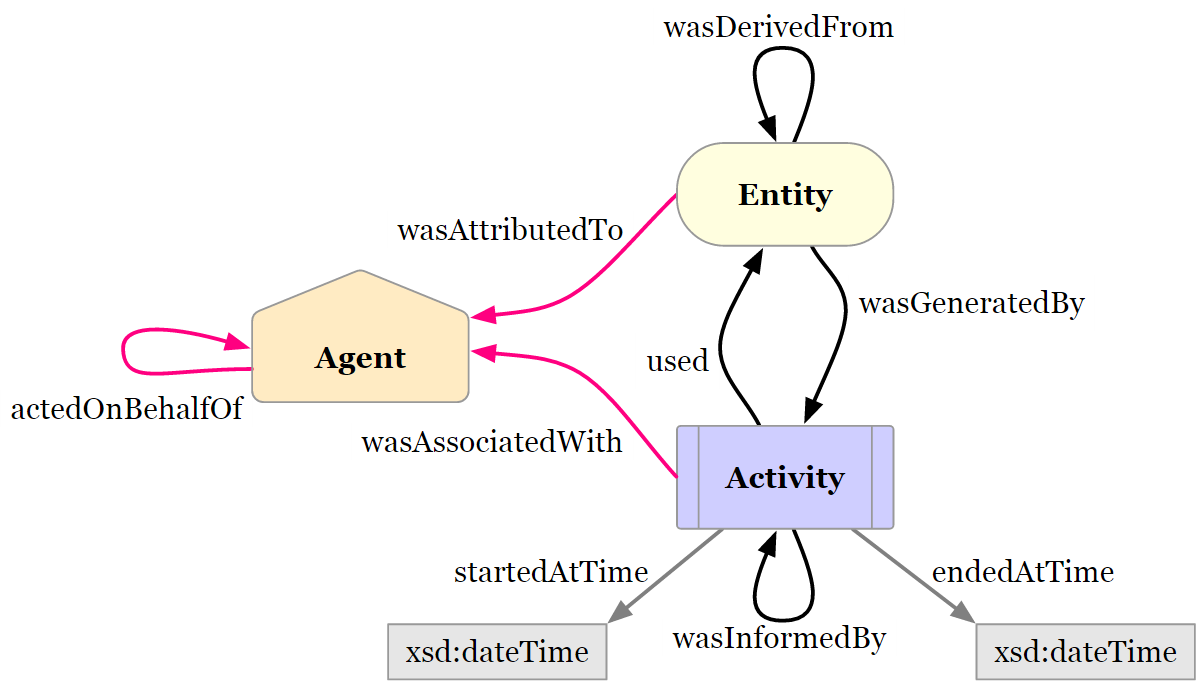
\includegraphics[width=\textwidth]{images/ProvLinchpin.png}
  \caption{Linchpin of the Provenance Ontology: Entities, Agents, Activities \cite{prov}}
  \label{fig:prov}
\end{figure}

%Provenance information is needed in any given scenario. 
In the context of datasets, provenance information on the activities which helped to create a dataset, which agents were involved in these processes and who to contact about it as well as source datasets or other entities involved are of interest, especially when trying to determain the trustworthiness of data. This ontology is "[...] the foundation to implement provenance applications in different domains that can represent, exchange, and integrate provenance information generated in different systems and under different contexts." \cite{prov}

Each of the relations depicted (\cref{fig:prov}) have suitable qualification classes (e.g. \prop{prov:Association}), so that a property (\prop{prov:wasAssociatedWith}) can be inferred from the qualified property path  (\prop{prov:qualifiedAssociation}/\prop{prov:agent}). Qualification classes provide qualification via properties such as \prop{prov:role}. 

In this example (from the official specification of \prov \cite{prov}), an association provides additional description about the :illustrationActivity that an agent named 'Derek' influenced:

\begin{lstlisting}[language=ttl, captionpos=b, label=lst:dcex,linewidth=\columnwidth,breaklines=true]
@prefix prov: 			<http://www.w3.org/ns/prov#> .
@prefix :     			<http://example.org#> .

:illustrationActivity
   a prov:Activity;                  ## this illustration activity was 
   prov:wasAssociatedWith :derek;    ##   associated with Derek in some way.
.

:derek a prov:Agent .

:illustrationActivity
   prov:qualifiedAssociation [       ## Qualify how the :illustrationActivity
      a prov:Association;            ##   was associated with the Agent Derek.
      prov:agent   :derek              

      prov:hadRole :illustrationist; ## Qualification: The role that Derek served
      prov:hadPlan :tutorial_blog;   ## Qualification: The plan (or instructions)
                                     ##   that Derek followed when creating 
   ].                                ##   the graphical chart.

:tutorial_blog   a prov:Plan, prov:Entity .
:illustrationist a prov:Role .
\end{lstlisting}

\prov will have a central role in the creation of DataID. Further reading on the key requirements, guiding principles, and design decisions which influenced the PROV Family of Documents\footnoteurl{https://www.w3.org/TR/2012/WD-prov-overview-20121211/} is advised (see \cite{MoreauProv2015}).

\subsection{Open Digital Rights Language (ODRL)}
\label{sec:odrl}
The Open Digital Rights Language (\odrl)\footnoteurl{https://www.w3.org/ns/odrl/2/ODRL21} is an initiative of the W3C community group with the same name\footnoteurl{https://www.w3.org/community/odrl/}, aiming to develop an open standard for policy expressions. 
The \odrl version 2.0 core model defines
licensing policies in regard to their permissions
granted, duties and constraints associated with these
permissions as well as involved legal parties. Thus, an \odrl
description allows to specify, in a machine-readable way, if
data can be edited, integrated or redistributed.

\subsection{Lexvo.org}
\label{sec:lexvo}
Lexvo.org\footnoteurl{http://www.lexvo.org} is a service publishing language related information as Linked Data on the Web. The data published is conform to the Lexvo Ontology, providing unique identifiers for human languages in the context of geography, language families, words and word senses, scripts and characters \cite{Lexvo2015DeMelo}. All in all, the Lexvo dataset consists of over 8000 languages with a broad spectrum of language-related information that is extensively used by many data publishers and communities.

\subsection{Friend of a Friend vocabulary (FOAF)}
\label{sec:foaf}
\cite{Brickley-2014} \todo{add foaf!}

\subsection{DataCite Ontology}
\label{sec:dcid}
DataCite is a "global non-profit organisation that provides persistent identifiers (DOIs) for research data [with the goal] to help the research community locate, identify, and cite research data with confidence"\footnoteurl{https://www.datacite.org/mission.html}. \todo{revise citation}

DataCite published an XML schema for describing and citing research data\footnoteurl{http://schema.datacite.org/meta/kernel-4.0/}, which is elaborate and at times novel approach for providing dataset metadata. Yet, due to its rigid XML structure with many cardinality restrictions, it does not feature in my collection of dataset metadata in this chapter. 

Of more interest, is the DataCite ontology which was published as an OWL ontology\footnoteurl{http://www.sparontologies.net/ontologies/datacite/source.html} and has a particular focus on representing identifiers (\cref{fig:dcid}). The Identifier class is divided into ResourceIdentifier and AgentIdentifier. In addition, an IdentifierScheme defines the format of the literal which represents the identifier. As opposed to an approach with data-types, this ontology allows for adding new schemes without altering the vocabulary itself and adding additional qualifications to the scheme entity \cite{Peroni2016}. Furthermore, the DataCite ontology contains a multitude of predefined IdentifierScheme instances, ready to be used. 


\begin{figure}[t]
\centering
  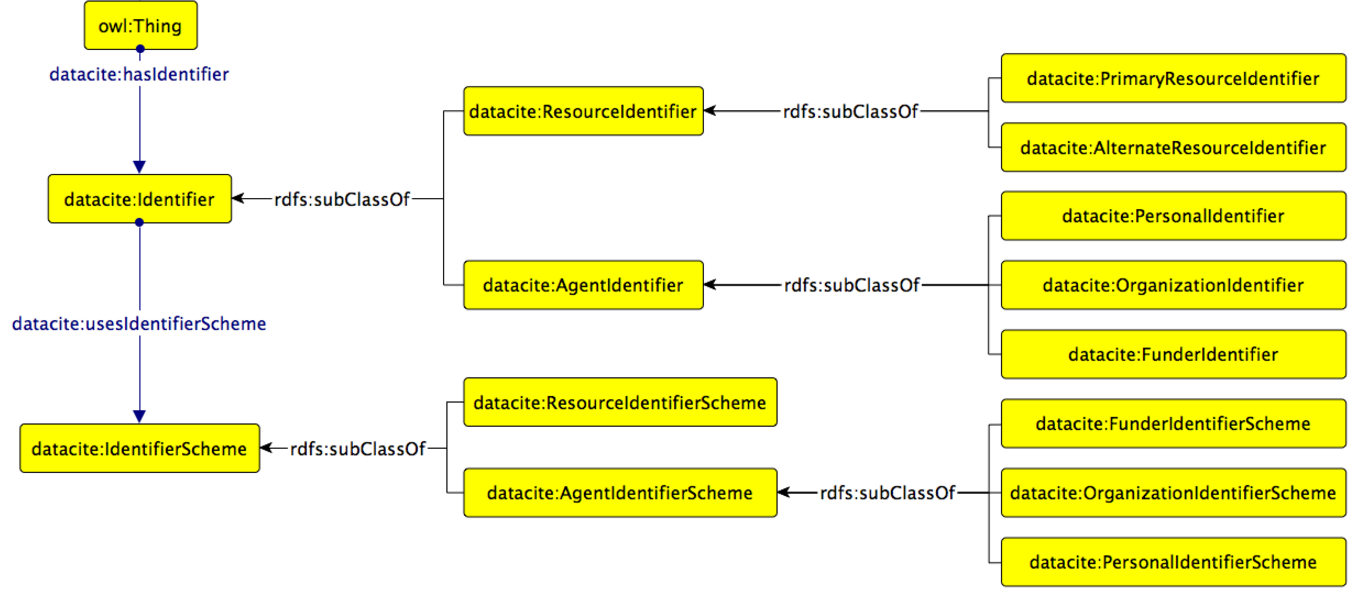
\includegraphics[width=\textwidth]{images/DataCiteIdentifiers.png}
  \caption{DataCite Identifier and IdentifierScheme}
  \label{fig:dcid}
\end{figure}

\subsection{DBpedia}
\label{sec:dbpedia}

DBpedia is a community effort to extract structured information from Wikipedia and to make this information available on the Web, where it is used as a common point of reference for interlinking and enriching most of the structured data on the web today, establishing it as the center of the so called 'LOD cloud'. \todo{this section needs polishing and references!}

The main focus of the DBpedia extraction lies in mapping of info boxes, templates and other easily identified structured data found in Wikipedia articles to properties of an ontology. The DBpedia ontology is reflecting the relations and classifications found within Wikipedia. Together with the mappings to the Wikipedia XML templates, this ontology is curated by a community of interested people around the world to update schematical changes in time for the bi-yearly DBpedia releases. 

Each release consists of around one hundred datasets for each of its 130 (2016) language editions (reflecting most of the languages of Wikipedia). Datasets are often created around particular properties (such as \prop{rdf:type}) or other distinguishing features. To reflect this large corpus of structured data, the need for specific demands on its metadata are self-evident.

\todo{probably gets another field on the data quality vocabulary...}

\chapter{The DataID Ecosystem}
\label{chap:ecosystem}

\section{Problem Statement} 
\label{sec:probstat}
%Modularizing the original ontology into multiple layers, making DataID independent to the type of data in the process. By augmenting the core ontology with multiple existing extensions and use case specific additions we underline the capabilities in regard to

The inadequacies of current metadata vocabularies are manifold and diverse (\cref{sec:dv}). As already introduced (\cref{sec:motivation}), there are some issues which protrude from the rest, due to their ubiquitousness in use cases or their import on aspects like interoperability, trustworthiness and governance of data.

This list of important aspects of metadata reflects these issues and explains them in detail:

\textbf{(A1)} \provenance: a crucial aspect of data, required to assess correctness and completeness of data conversion, as well as the basis for trustworthiness of the data source (no trust without provenance). 

\textbf{(A2)} \licensing: machine-readable licensing information provides the possibility to automatically
%process, integrate and publish 
publish, distribute and consume only data that explicitly allows these actions. %%\todo{instead of "process, integrate and publish" could we use the same name as the permissions in \odrl to be consistent?, MF: not sure if these are the ones you meant..., process, integrate and publish  is directly from the first DataID paper and i think are more to the point}

\textbf{(A3)} \access: publishing and maintaining
this kind of metadata together with the data itself serves as
documentation benefiting the potential user
of the data as well as the creator by making it discoverable
and crawlable. 

\textbf{(A4)} \extensibility: extending a given core metadata model
in an easy and reusable way, while leaving the original model uncompromised expands its application possibilities fitting many
different use cases. 

\textbf{(A5)} \interoperability: the interoperability with other metadata models is a hallmark for a widely usable and reusable dataset metadata model.

When regarding aspects \textbf{(A4)} and \textbf{(A5)}, taking into account the intricate requirements of many use cases (such as in \Cref{requDmp})\todo{update ref}, \extensibility and \interoperability seem contradictory when leaving the more general levels of a domain description. A vocabulary capable of interacting with other metadata vocabularies might be too general to fit certain scenarios of use. Restrictive extensions to a vocabulary might encroach on its ability to translate into other useful metadata formats. This notion is corroborated by this document~\cite{ivse}. Note: I do not differentiate between \evolvability and \extensibility (as done in this source) in the context of this thesis. The discrepancies with \interoperability are true for both concepts. Letting features 'die out' over time does not impact, in my understanding, the aspect of \extensibility. 

We conclude, not only is there a gap between existing dataset metadata vocabularies and requirements thereof, but it seems unlikely that we are able to solve all these diverse problems with just one, monolithic ontology.

%We conclude, that a gap exists between existing dataset metadata vocabularies and what is required.
%Hence it seems unlikely that we are able to solve all these diverse problems with just a single, monolithic ontology.
%Extending a vocabulary for a certain use case will in most cases result in singular, non reusable solutions to a problem. Restrictive extensions of metadata 


\section{The multi-layer ontology of DataID} % 2 pages
\label{sec:multilayer}

%KM: Added ", which" and "section,"
While trying to solve the different aspects, which we discussed in the previous section, and tending to the needs of different usage scenarios, the DataID ontology grew in size and complexity.

%To ,
In order to keep the \dataid ontology reasonable in size and complexity as well as not to jeopardise \extensibility and \interoperability, we modularised \dataid in a core ontology and multiple extensions. The onion-like layer model (\cref{fig:onion}) illustrates the import dependencies between the ontologies: 

\begin{figure}[!htbp]
\centering
  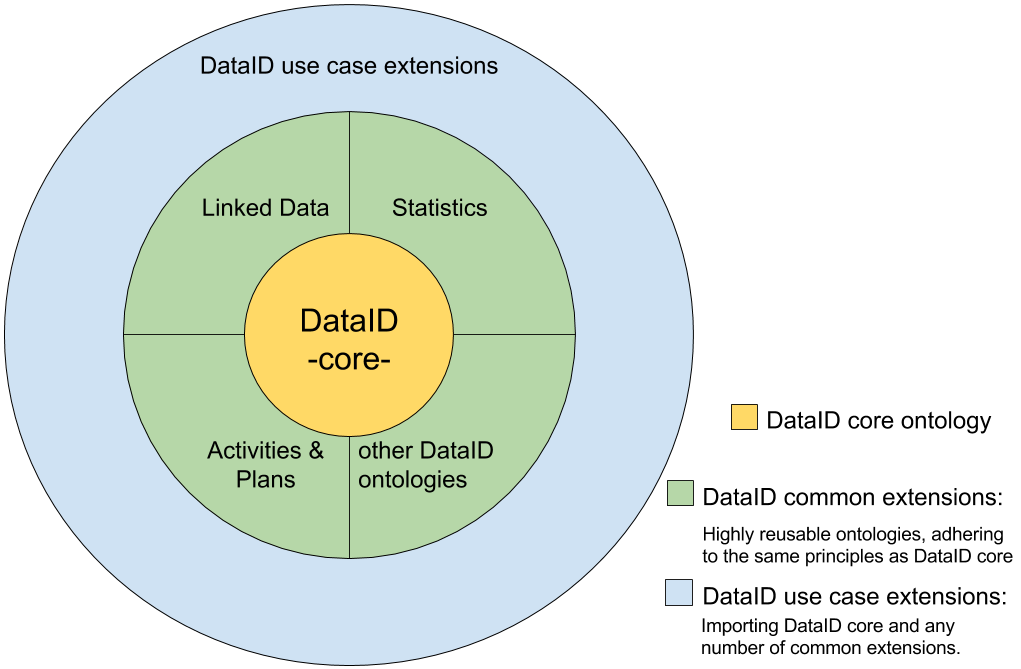
\includegraphics[width=\textwidth]{images/DataIDonion.png}
  \caption{The Metadata Ecosystem of DataID}
  \label{fig:onion}
\end{figure}

The scaling approach used to modularize the original \dataid ontology adopts principles of the modular programming technique, separating concepts and properties of a large ontology into independent, interchangeable modules, specialised to fit common use cases, dependent only on \core. Thus, any vocabulary in this sphere must import \core, with the exception of \core itself. 
The mid-layer (or common extensions) of this model is comprised of highly reusable ontologies, extending \core to cover additional aspects of dataset metadata. Non of these are mandatory imports for any ontology, yet, in many cases some or all of them will be useful contributions. While I will not (and can not) impose any restrictions as to which ontologies not to import, ideally, ontologies of this layer should only import \core, to minimize discrepancies between mid-layer ontologies of different authors with overlapping purposes. The outermost layer of this sphere represents all vocabularies importing \core and any number if mid-layer ontologies and adding additional semantics to portray domain or use case specific demands for metadata.

The \ecosystem is a suite of ontologies comprised of \core and its extensions, which were created to satisfy different use cases in a reusable manner. The brackets enclosed namespace prefixes are recommended and used throughout this work:

\begin{description}
\item[DataID core (dataid)] provides the basic description of a dataset (cf. \Cref{sec:coreintro}) and serves as foundation for all extensions to DataID.
\item[Linked Data (dataid-ld)] extends DataID core with an interface for the Sparql Service Description vocabulary \cite{sparqlsd}, which not only allows to specify SPARQL endpoints, but offers properties useful for Linked Data datasets as well (such as \prop{sd:defaultGraph})\footnoteurl{https://github.com/dbpedia/DataId-Ontology/tree/master/ld}. While the \void vocabulary is already imported in \core (see \cref{sec:coreintro}), many \void and properties only become useful in this context (e.g. \prop{void:triples}). I introduced a specialised sub classes (\prop{dataid-ld:LinkedDataDataset}) to better distinguish datasets of this focus. 
\item[Activities \& Plans (dataid-acp)] provides provenance information of activities which generated, changed or used datasets\footnoteurl{https://github.com/dbpedia/DataId-Ontology/tree/DataManagementPlanExtension/acp}. The goal is to record all activities needed to replicate a dataset as described by a DataID. Plans can describe which steps (activities, precautionary measures) are put in place to reach a certain goal. This extension relies heavily on the \prov ontology\cite{prov}.
\item[Statistics (dataid-md)] will provide the necessary measures to publish multi-dimensional data, such as statistics about datasets, based on the Data Cube Vocabulary\cite{datacube}. 
\item[Other common extensions] of similar general character as the ontologies of that layer, which could be useful in multiple use cases.
\end{description}

Ontologies under the DataID multilayer concept do not offer cardinality restrictions, making them easy to extend and adhere to OWL profiles. An application profile for \core (cf. \Cref{lessons}) was declared using SHACL \cite{shacl}.

Extending this ecosystem of dataset metadata with domain-specific OWL ontologies adds further opportunities for applications clustered around datasets, as we will showcase in \Cref{dmps}.\todo{ref}


\section{The interplay of ontologies} 
\label{sec:interplay}\todo{title will be revised}
Multiple requirements are planned to be enforced for the adoption of new ontologies in the common (or mid) layer of the DataID Ecosystem.
They might contain (while not being restricted to):

\begin{itemize}
\item Authors must provide information about the reason for the new extension (and why the expected result is not achievable with existing extensions).
\item Authors must document the Interoperability with other extensions of this layer (and where problems are to be expected).
\item Authors must inform about conformity with OWL profiles.
\end{itemize}

Deciding on which combination of DataID ontologies to use for a Dataset description is a domain and problem dependent process. It may be necessary to add additional properties on top of the provided metadata properties.

\begin{figure}[!htbp]
\centering
  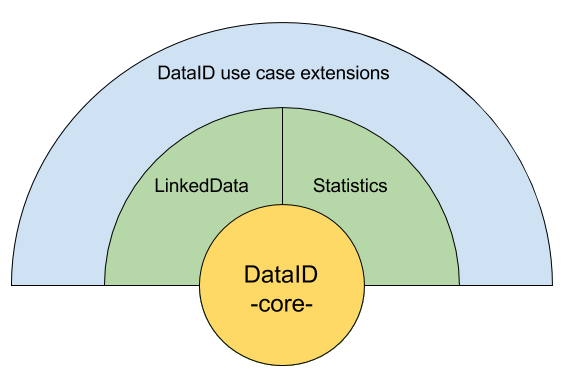
\includegraphics[width=9cm]{images/DataIDonionSliced.png}
  \caption{Example of combining multiple DataID ontologies}
  \label{fig:onionslice}
\end{figure}

For example, a DataID based ontology for LOD Datasets dealing with multi-dimensional data, may look schematically like this:
(importing DataID core and the extensions for Linked Data and Statistics, as well as some additional properties only used in the use case at hand.)

\chapter{DataID core Ontology}
\label{cahp:core}

\section{Overview} 
\label{sec:coreintro}

This section will provide an overview of the \core ontology and some background on basic design decisions made. Most of the vocabularies reused by this ontology have already been presented in \cref{chap:relatedwork} and need no further introduction.

\core developed out of a previous version of \dataid by following the aspiration to modularise \dataid into a core-ontology, surrounded by its dependents. Many design decisions of \core were already introduced in its former version, which was designed to make \dcat, combined with the \void vocabulary, fit the requirements of the DBpedia use case for a hierarchy of Linked Data datasets (see also \cref{sec:dbpedia}):

\begin{quote}
"The DBpedia dataset, with
its different versions and languages, multiple SPARQL endpoints
and thousands of dump files with various content
serves as one example of the complexity metadata models
need to be able to express. We argue that the DCAT vocabulary
as well as the established VoID vocabulary only
provide a basic interoperability layer to discover data. In
their current state, they still have to be expanded to fully
describe datasets as complex as DBpedia [...]." \cite{dataID2014} 
\end{quote}

\core is founded on two pillars: the \dcat and \prov ontologies. To incorporate \dcat as the basis of \dataid, to further extend \dcat with \prov, introducing extensive provenance records in the process, and adding properties specific to the DBpedia use case was the original premise of this endeavour. In addition, the \void vocabulary was adopted to cover Linked Data specific semantics and provide more general properties, such as  \prop{void:subset} for establishing dataset hierarchies. The wide application of these vocabularies in the context of the Semantic Web was the rational behind these decisions, furthering our goal of \interoperability. 

\begin{figure}[!htbp]
\centering
  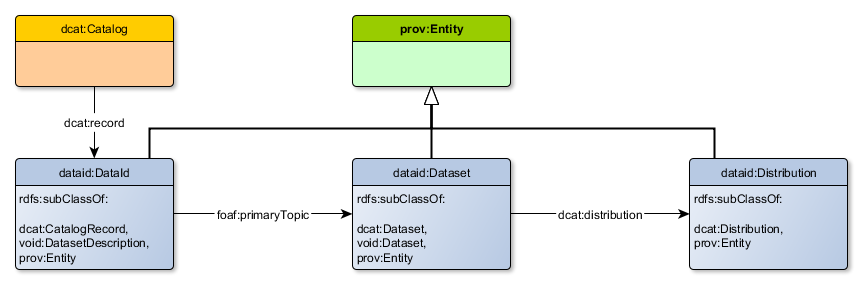
\includegraphics[width=\textwidth]{images/FoundationalConcept.png}
  \caption{Foundations: Combining \dcat, \void and \prov}
  \label{fig:foundations}
\end{figure}

As \dcat, \core is centred around the Dataset and Distribution concepts which were imported from \dcat. We introduced the class \prop{dataid:DataId} (see \cref{sec:coredataid}), merging both \prop{dcat:CatalogRecord} and \prop{void:DatasetDescription} into one, and providing an additional level of abstraction between \prop{dataid:Dataset} and \prop{dcat:Catalog}. Instances of this class can be compared to root elements in the XML world, since all subsequent instances, describing a dataset, are hierarchicaly below a DataId instance. Though, this comparison is of course misleading, since a graph has no orientation. Yet, most of DataID documents\footnote{DataID graph serialised as a metadata document} will have structural similarities to XML documents.

All dataset related classes of \core (\prop{dataid:DataId}, \prop{dataid:Dataset} and \prop{dataid:Distribution}) are sub classes of \prop{prov:Entity}, which is the interface needed to harness the possibilities of the Provenance Ontology (\prov). In the context of this description of \core, the word 'Entity' is used to refer to instances of \prop{prov:Entity} (ergo: instances of these three classes).

With \prov, describing the circumstance of provenance for any domain is possible (\cref{sec:prov}). Central to this, is the concept of qualification classes, providing qualifications for more general properties (e.g. for \prop{prov:wasAttributedTo}). Describing the interrelations between Entities (such as a particular dataset or just a single distribution of it) and Agents (e.a. a person or an organisation) are salient requirements in most environments for datasets and their metadata. Thus, \core has singled out these relations to further qualify them and provide much needed referential integrity.\todo{explain}

For example, the property \prop{dataid:associatedAgent} (which is a sub property of \prop{prov:wasAttributedTo}) is a universal relation between an Entity and an Agent. It can (and should) be qualified by an instance of \prop{dataid:Authorization}, a sub class of \prop{prov:Attribution}. An Authorization adds qualifications and restrictions to the original property, such as an agent role (defining the role the agent has in regard to the Entities involved - see \cref{sec:coreauthorization}). core allows for assigning Actions to an Authorization, which specify what an Agent can do and for which tasks he/she/it is responsible for.

\begin{figure}[!htbp]
\centering
  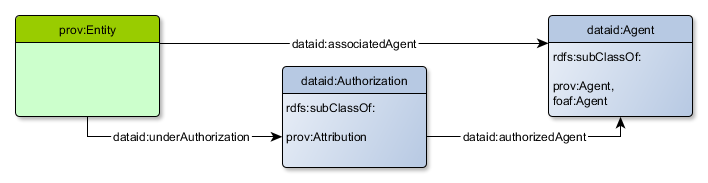
\includegraphics[width=\textwidth]{images/FoundationalConseptProv.png}
  \caption{Foundations: Using \prov to qualify properties}
  \label{fig:foundations}
\end{figure}

In its current version 2.0.0, \core offers a general approach for describing dataset metadata, incorporating important ontologies to extend \dcat with \provenance, qualifying relations and their intended range classes, hierarchical dataset structures, management of rights and responsibilities of agents and exhaustive descriptions for data \access. 

In general, \core waived the use of cardinality restrictions\footnote{this is the purpose of an application profile, not of an ontology}, making it easier to adhere to the OWL 2 RL\footnoteurl{https://www.w3.org/TR/owl2-profiles/#OWL_2_RL} profile and maintaining the benefits of easy \extensibility and \interoperability prevalent with \dcat. In turn, \core restricts some of the very general property ranges of Dublin Core and \dcat properties (such as \prop{dct:license} or \prop{dcat:mediaType}), to reduce impreciseness and increase machine-readability.

\core is making use of the following namespace:
\begin{lstlisting}[language=ttl, label=lst:graph,linewidth=\columnwidth,breaklines=true,basicstyle=\ttfamily\footnotesize]
http://dataid.dbpedia.org/ns/core#
\end{lstlisting}
At this URI, an extended description of each class and property, introduced by this ontology, can be found as well as the complete ontology specification in Turtle\footnoteurl{http://dataid.dbpedia.org/ns/core.ttl} or OWL\footnoteurl{http://dataid.dbpedia.org/ns/core.owl} serialization.\todo{should i put the whole specification in the appendix? would be about 20 pages...}

For a better understanding of the imported concepts and properties, which are reused by \core, I would advise to read up on \dcat \cite{ddcat} and \prov \cite{prov} (since these are used most commonly), to gain a more complete picture of the underlying structure and rational of these ontologies. While I gave a concise introduction to both in \cref{sec:dcat} and \cref{sec:prov} respectively, this work is not the space to repeat this in more detail.

\begin{figure}
\centering
	\vspace*{-0.8cm}
  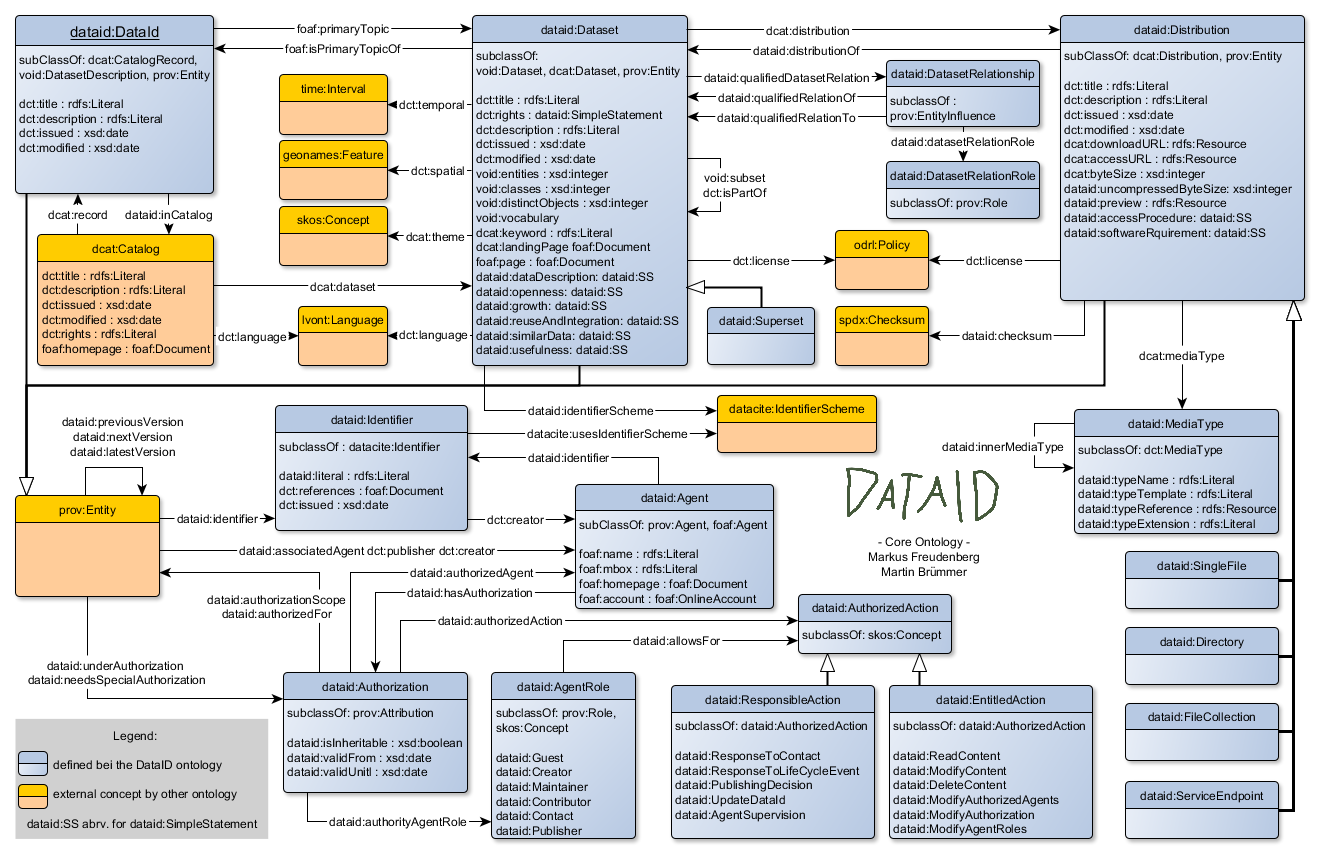
\includegraphics[angle=90, width=\textwidth]{images/DataIdOntology.png}
  \caption{\core}
  \label{fig:core}
  %\floatfoot{An exact description of all classes and properties can be found under the DataID namespace uri \url{http://dataid.dbpedia.org/ns/core} including this depiction. The ontology RDF document is also available there:
  %\url{http://dataid.dbpedia.org/ns/core.ttl} (.owl)}
\end{figure} 

\pagebreak
\section{Classes} 
\label{sec:coreclasses}

This section is partitioned by concepts to introduce the \core ontology. Each class is presented with an item of written comment about the general reasoning behind its existence and its intended use.
For illustration purposes, a running example was woven into the descriptions of concepts and properties. This example is a reduced version of an original \dataid document of the Arabic DBpedia (release: 2015-10\footnoteurl{http://}). Under the main dataset, only two sub-datasets are shown (as opposed to over 50 in the real world example from which this is drawn). It was chosen to cover many aspects of \core and to provide an easy use case which could arise in a similar fashion outside the DBpedia domain. The full example is available in Turtle serialisation\footnoteurl{http://} in Appendix I. The basic structure of its \dataid document is outlined below (\Cref{fig:example}).

\begin{figure}[!htbp]
\centering
  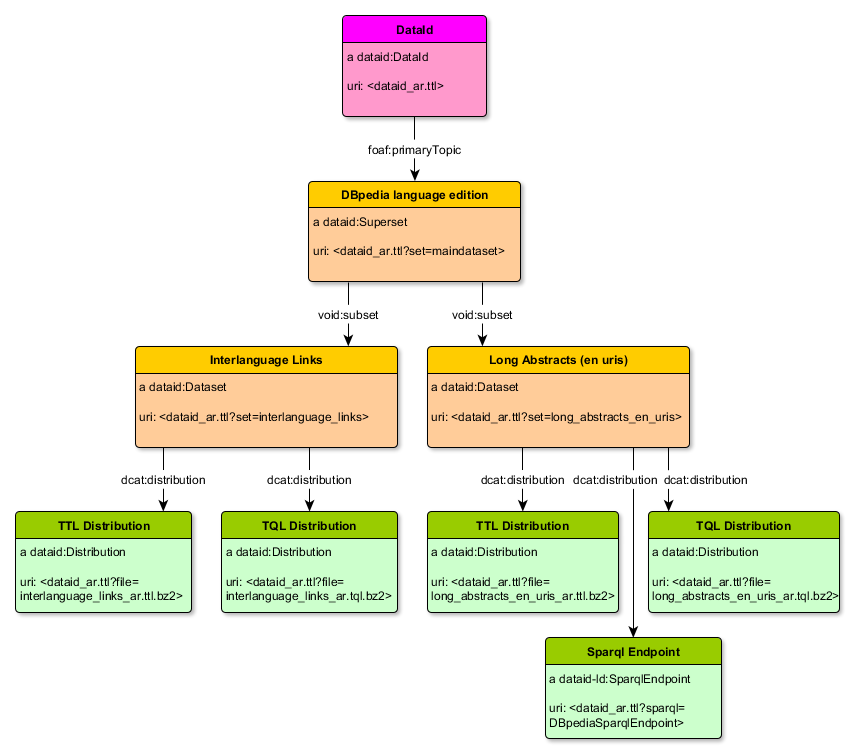
\includegraphics[width=13cm]{images/ExampleStructure.png}
  \caption{Schematic view: A shallow hierarchy of Datasets.}
  \label{fig:example}
\end{figure}

For the purpose of this running example the following base URI was used to shorten all subsequent URIs of this:
\begin{lstlisting}[language=ttl,label=lst:graph,linewidth=\columnwidth,breaklines=true,basicstyle=\ttfamily\footnotesize]
@base <http://downloads.dbpedia.org/2015-10/core-i18n/ar/2015-10_>
\end{lstlisting}

Some instances referenced in the example were left out to reduce redundancy.\todo{true?} The example omits the more common properties of Dublin Core\footnoteurl{http://} and RDFS\footnoteurl{http://} such as \prop{dct:title}, \prop{dct:description}, \prop{dct:modified}, \prop{dct:issued} and \prop{rdfs:label} to make this example more easy to read. 

In addition, this running example does not only use \core, it also introduces a first \dataid extension from the common layer of the \ecosystem (\cref{sec:multilayer}) for Linked Data datasets. The Linked Data extension\footnoteurl{https://github.com/dbpedia/DataId-Ontology/tree/master/ld} (prefix: dataid-ld) is used to describe dataset attributes, specific to Linked Data.

The remainder of this section features each subsection with a short summary, stating the purpose of each concept, a list of properties commonly used to describe instances of this concept, a schematic depiction of the concept, followed by at least one example instance of this class (taken from the running example of DBpedia). The list of properties features a rating for each property to advise whether an application profile based on \core should declare a property to be: mandatory \textbf{(M)}, recommended \textbf{(R)} or optional \textbf{(O)}.


\subsection{DataId} 
\label{sec:coredataid}
The class \prop{dataid:DataId} inherits from \prop{dcat:CatalogRecord}, which does not represent a dataset, but metadata about a dataset's entry in a catalogue. Additionally, in the context of \core, it represents metadata about a \dataid document (graph), such as version pointers, modification dates and relations to its context (such as Agents, Catalogues, Repositories). This DataId resource is the most abstract Entity in any \dataid graph. 

\begin{figure}[!htbp]
\centering
  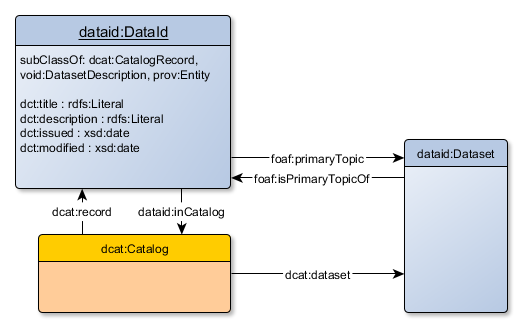
\includegraphics[width=10cm]{images/ClassDataId.png}
  \caption{Class DataId}
  \label{fig:example}
\end{figure}

Properties specifically used with \prop{dataid:DataId}:
\begin{description}
\item[\prop{dataid:inCatalog}:] the inverse of \prop{dcat:record} references the \dcat catalogue a \dataid is entered in. \textbf{(R)}
\item[\prop{foaf:primaryTopic}:] this functional property is used to point out the dataset resource this \dataid represents. \textbf{(M)}
\end{description}

In addition, the following list contains properties which can be used with any Entity and are presented here for convenience:
\begin{description}
\item[\prop{dataid:associatedAgent}:] points out all agents which have some (unspecified) influence (or authority) over this Entity. \textbf{(O)}
\item[\prop{dataid:underAuthorization}:] refers an instance of \prop{dataid:Authorization} which qualifies the generic \prop{dataid:underAuthorization} relation (see \cref{sec:coreauthorization}). \textbf{(R)}
\item[\prop{dct:publisher}:] While the \prov based way to declare associated agents and their roles in regard to this Entity is in place, using established properties to point out agents (such as \prop{dct:publisher}) is not redundant and should be kept as best practice. \textbf{(R)}
\item[\prop{dataid:nextVersion}:] is used to identify instances of the same type (in this case \prop{dataid:DataId}), which are next in the chain of different versions of this resource. \textbf{(O)}
\item[\prop{dataid:previousVersion}:] points out the previous version of this instance. \textbf{(R)}
\item[\prop{dataid:latestVersion}:] points out the latest version of this instance. \textbf{(R)}
\end{description}

The example below illustrates the use of this concept. It provides a pertaining dataset catalogue (via \prop{dataid:inCatalog}), uses version pointers to define its position in a branch of a versioning system, points out agents and authorizations and the dataset about which this \dataid is about (\prop{foaf:primaryTopic}).

\pagebreak
\begin{lstlisting}[language=ttl, captionpos=b,caption=Instance of a DataId,label=lst:coredataid,linewidth=\columnwidth,breaklines=true]
<dataid_ar.ttl>
        a                          dataid:DataId ;
        dataid:associatedAgent     <http://wiki.dbpedia.org/dbpedia-association> ;
        dataid:inCatalog           <http://downloads.dbpedia.org/2015-10/2015-10_dataid_catalog.ttl> ;            
        dataid:latestVersion       <http://downloads.dbpedia.org/2016-04/core-i18n/ar/2016-04_dataid_ar.ttl> ;
        dataid:nextVersion         <http://downloads.dbpedia.org/2016-04/core-i18n/ar/2016-04_dataid_ar.ttl> ;    
        dataid:previousVersion     <http://downloads.dbpedia.org/2015-04/core-i18n/ar/2015-04_dataid_ar.ttl> ;
        dataid:underAuthorization  <dataid_ar.ttl?auth=creatorAuthorization> ;                                    
        dct:hasVersion              <dataid_ar.ttl?version=1.0.0> ;
        dct:publisher               <http://wiki.dbpedia.org/dbpedia-association> ;                                
        dct:title                   "DataID metadata for the Arabic DBpedia"@en ;
        foaf:primaryTopic          <dataid_ar.ttl?set=maindataset>
\end{lstlisting}

\subsection{Dataset} 
\label{sec:coredataset}
This is the central concept of the \core ontology and offers a multitude of useful properties to describe a dataset comprehensively.
\begin{figure}[!htbp]
\centering
  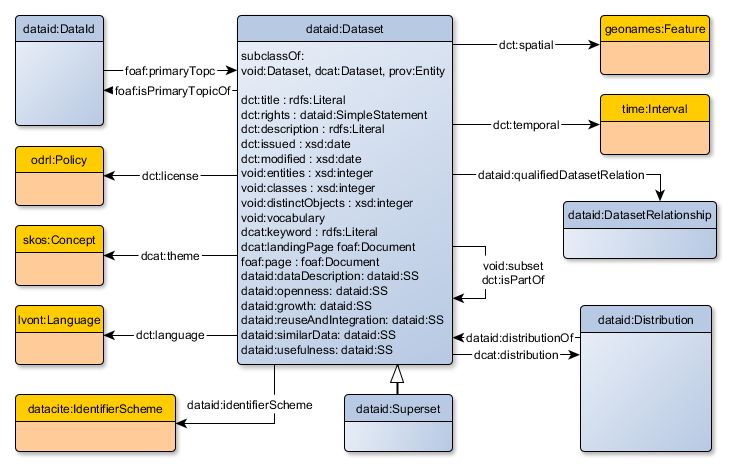
\includegraphics[width=\textwidth]{images/ClassDataset.png}
  \caption{Class Dataset}
  \label{fig:example}
\end{figure}

The dataset concept of both the \dcat and \void were merged into \prop{dataid:Dataset}, providing useful properties about the content of a dataset from both ontologies. In particular, the property \prop{void:subset} allows for the creation of dataset hierarchies, while \prop{dcat:distribution} points out the distributions of a dataset. The \prop{dataid:Superset} as a subclass of \prop{dataid:Dataset} shall be used to represent multiple sub-dataset entities, portraying dataset collections or hierarchical dataset structures in general. Opposed to a conventional Dataset, a Superset is prohibited from possessing Distributions (referred to with \prop{dcat:distribution}). It is strongly recommended that each Dataset shall either have at least one Distribution or one Sub-Dataset. 

In the running example, the main dataset (an instance of \prop{dataid:Superset}), is used as a hierarchical root, representing all Sub-Datasets clustered around a common topic. In the case of DBpedia, all Datasets were arranged under a Superset representing a DBpedia language edition.

Properties commonly used with instances of this class are:
\begin{description}
\item[\prop{dcat:distribution}] provides the distributions of a dataset and should be used distinct from \prop{void:subset}. \textbf{(M for non Supersets)}
\item[\prop{void:subset}] is the property used to reference sub datasets which are part of a superset. Its use is limited to \todo{void subset only for superste???}the sub class \prop{dataid:Superset}. \textbf{(M if Superset)}
\item[\prop{dct:license}] as already stated (\cref{ddd}), this property is restricted in the context of \dataid to instances of the class \prop{odrl:Policy} of the \odrl ontology, providing machine-readable licensing information. \textbf{(M)}
\item[\prop{dct:language}:] This property from the Dublin Core vocabulary is used to point out the predominant language used within a dataset. Since a \prop{rdfs:range} statement is not provided, even literals could be used with this predicate. \core restricts the range of this property to instances of  lvont:Language, a class from the Lexvo ontology (see \cref{sec:lexvo}), describing human languages in a machine readable way. \textbf{(R)}
\item[\prop{void:vocabulary}] in the \void vocabulary, this property is used to point out the associated ontology used to create a dataset. \core broadens its use case so that any schema document (e.g. XSLT or database schemata) can be pointed out, depending on the type of data. \textbf{(R)}
\item[\prop{foaf:page}] is commonly used to point out web pages which have the function of a manual or documentation for the resource at hand. \textbf{(R)}
\item[\prop{dct:rights}] this property is used to provide a statement or resource about issues like copy rights or legal notes. To avoid unqualifiable literal statements, this property is reduced to \prop{dataid:SimpleStatement}. \textbf{(O)}
\item[\prop{foaf:isPrimaryTopicOf}] is the inverse property of \prop{foaf:primaryTopic} (see \cref{sec:coredataid}). \textbf{(O)}
\item[\prop{dataid:relatedDataset}:] generic pointer to related datasets (sub property of \prop{dct:relation}), qualifiable by \prop{dataid:qualifiedDatasetRelation}. Refer to \cref{sec:coredatasetrelationship} for more. \textbf{(O)}
\item[\prop{dataid:qualifiedDatasetRelation}] provides an instance of concept \prop{dataid:DatasetRelationship} which is a qualification class for the generic property \prop{dataid:relatedDataset} \textbf{(O)}
\item[\prop{dataid:identifierScheme}:] provides a resource describing the identifiers used within the dataset to uniquely identify a record (data point, datum). Refer to \cref{sec:coreidentifier} to learn more about Identifiers. \textbf{(O)}
\item[\prop{dcat:keyword}:] a simple keyword or tag associated with this dataset \textbf{(O)}
\item[\prop{dcat:landingpage}:] references a web page of general character (such as the homepage of an organisation) \textbf{(O)}
\end{description}

Multiple properties for textual statements on different aspects of a Dataset were created. All of which provide publishers, maintainers and other agents a way to convey statements of general character on such subjects as described below. This information will be useful in many scenarios related to dissemination tasks, for example, those described by the Horizon 2020\footnoteurl{https://ec.europa.eu/programmes/horizon2020/} data management plan guidelines\footnoteurl{https://ec.europa.eu/research/participants/data/ref/h2020/grants_manual/hi/oa_pilot/h2020-hi-oa-data-mgt_en.pdf} (more on this in \cref{chap:dmp}).

All of these properties are listed below have the common \prop{rdfs:range} of \prop{dataid:SimpleStatement}, which allows to either provide a literal or reference a web page containing the textual information about the resource (see \cref{sec:corestatement}). 

\begin{description}
\item[\prop{dataid:dataDescription}:] provides a detailed textual description of the data represented by this Dataset. \textbf{(O)}
\item[\prop{dataid:growth}:] indication of what size the approximated end volume of the Dataset is. \textbf{(O)}
\item[\prop{dataid:usefulness}:] is used to state to whom the Dataset could be useful, and whether it underpins a scientific publication. \textbf{(O)}
\item[\prop{dataid:similarData}:] a statement on the existence (or absence) of similar data (see also \prop{dataid:relatedDataset}). \textbf{(O)}
\item[\prop{dataid:reuseAndIntegration}:] information on the possibilities for integration and reuse of the Dataset. \textbf{(O)}
\item[\prop{dataid:openness}:] General description of how data will be shared. For example embargo periods (if any), outlines of technical mechanisms for dissemination or a definition of whether access will be widely open or restricted to specific groups. In case the Dataset cannot be shared, the reasons for this should be mentioned (e.g. ethical, rules of personal data, intellectual property, commercial, privacy-related, security-related). \textbf{(O)}
\end{description}

The running example is structured in a shallow hierarchy with an instance of \prop{dataid:Superset} representing all dataset of a Arabic DBpedia language edition:
\\
\begin{lstlisting}[language=ttl, captionpos=b,caption=Instance of a Superset,label=lst:coresuperset,linewidth=\columnwidth,breaklines=true]
<dataid_ar.ttl?set=maindataset>
        a                           dataid:Superset ;
        dataid:associatedAgent      <http://wiki.dbpedia.org/dbpedia-association>  ;
        dataid:growth               <dataid_ar.ttl?stmt=growth> ;                                                 
        dataid:openness             <dataid_ar.ttl?stmt=openness> ;
        dataid:reuseAndIntegration  <dataid_ar.ttl?stmt=reuseAndIntegration> ;
        dataid:similarData          <dataid_ar.ttl?stmt=similarData> ;
        dataid:usefulness           <dataid_ar.ttl?stmt=usefulness> ;
        dct:hasVersion               <dataid_ar.ttl?version=1.0.0> ;
        dct:language                 <http://lexvo.org/id/iso639-3/ara> ;                                          
        dct:license                  <http://purl.oclc.org/NET/rdflicense/cc-by-sa3.0> ;  
        dct:publisher                <http://wiki.dbpedia.org/dbpedia-association> ;
        dct:rights                   <dataid_ar.ttl?rights=dbpedia-rights> ;
        void:subset                 <dataid_ar.ttl?set=long_abstracts_en_uris>, 
        <dataid_ar.ttl?set=interlanguage_links> ;
        void:vocabulary             <http://downloads.dbpedia.org/2015-04/dbpedia_2015-10.owl> ;                  
        dcat:keyword                "maindataset"@en , "DBpedia"@en ;
        dcat:landingPage            <http://dbpedia.org/> ;                                                       
        foaf:isPrimaryTopicOf       <dataid_ar.ttl> ;                                                             
        foaf:page                   <http://wiki.dbpedia.org/Downloads2015-10> .  
\end{lstlisting}

This dataset has no distributions, the data it represents is referred to via its sub datasets. As an example for one of its sub datasets, the following listing exemplifies this difference:
\\
\begin{lstlisting}[language=ttl, captionpos=b,caption=A Dataset,label=lst:coresuperset,linewidth=\columnwidth,breaklines=true]
<dataid_ar.ttl?set=long_abstracts_en_uris>
        a                       dataid:Dataset, dataid-ld:LinkedDataDataset ;
        dataid:associatedAgent  <http://wiki.dbpedia.org/dbpedia-association> ;
        dataid:qualifiedDatasetRelation   <dataid_ar.ttl?relation=source&target=pages_articles> ;                 
        dataid:relatedDataset   <dataid_ar.ttl?set=pages_articles> ;
        dct:hasVersion           <dataid_ar.ttl?version=1.0.0> ;
        dct:isPartOf             <dataid_ar.ttl?set=maindataset> ;                                                 
        dct:language             <http://lexvo.org/id/iso639-3/ara> ;
        dct:license              <http://purl.oclc.org/NET/rdflicense/cc-by-sa3.0> ;
        dct:title                "long abstracts en uris"@en ;
        void:rootResource       <dataid_ar.ttl?set=maindataset> ;
        void:triples            232801 ;                                                                          
        void:sparqlEndpoint      <http://dbpedia.org/sparql> ;                                                    
        dcat:distribution       <dataid_ar.ttl?sparql=DBpediaSparqlEndpoint> ,                                    
            <dataid_ar.ttl?file=long_abstracts_en_uris_ar.ttl.bz2> ,
            <dataid_ar.ttl?file=long_abstracts_en_uris_ar.tql.bz2> ;
        dcat:keyword            "long_abstracts_en_uris"@en , "DBpedia"@en ;
        dcat:landingPage        <http://dbpedia.org/> ;
        sd:defaultGraph         <http://ar.dbpedia.org> ;                                                         
        foaf:page               <http://wiki.dbpedia.org/Downloads2015-10> . 
\end{lstlisting}

An instance of \prop{dataid-ld:LinkedDataDataset} with three distributions, representing two different RDF serialisations (Turtle - .ttl and Quad-Turtle - .tql) as well as an SPARQL endpoint. Furthermore, a source dataset (out of which this dataset was created) is referenced directly with \prop{dataid:relatedDataset}. The actual type of this relation (it being a \prop{dataid:SourceRelation}) will be evident by the qualified version described with the object of \prop{dataid:qualifiedDatasetRelation}. As a Linked Data dataset, properties such as \prop{void:triples} or \prop{sd:defaultGraph} can be applied.
 
\subsection{Distribution} 
\label{sec:coredist}

The class \prop{dataid:Distribution} provides the technical description of the data, the 'manifestation' of a dataset. In addition, it serves as documentation of how to access the data described (e.g. \prop{dcat:accessURL}), and which conditions apply (e.g. \prop{dataid:accessProcedure}). Every Distribution of a Dataset must contain all data of the Dataset in the format and location described. It may contain additional data exceeding the defined Dataset, for example when describing a service endpoint. Two Distributions of the same Dataset, therefore, must either contain the exact same data (for example in two different serialisations), or one Distribution must completely subsume the other. The Distribution concept, introduced by the \dcat vocabulary, is crucial to be able to automatically retrieve and use the data described in a \dataid document, simplifying, for example, data analysis. Additional sub classes, to further distinguish how the data is available on the Web, were introduced:

\begin{description}
\item[\prop{dataid:SingleFile}:] all data of a Dataset is available in a single file.
\item[\prop{dataid:Directory}:] the data of a Dataset is represented by the files in a single Directory on a file system.
\item[\prop{dataid:FileCollection}:] an arbitrary collection of (different files, not restricted to one file system), which in their accumulation represent the data of a Dataset.
\item[\prop{dataid:ServiceEndpoint}:] is a superclass for all service/api endpoints which could provide datasets. For example, REST APIs for databases\footnoteurl{https://docs.oracle.com/cloud/latest/mysql-cloud/CSMCS/index.html} or SPARQL endpoints for Triplestores.\todo{what is this?}
\end{description}

Except for \prop{dataid:SingleFile}, all of these subclasses may need additional semantics to describe them in a useful manner. This is not an objective of \core, further extensions of this ontology will address these issues.

\begin{figure}[!htbp]
\centering
  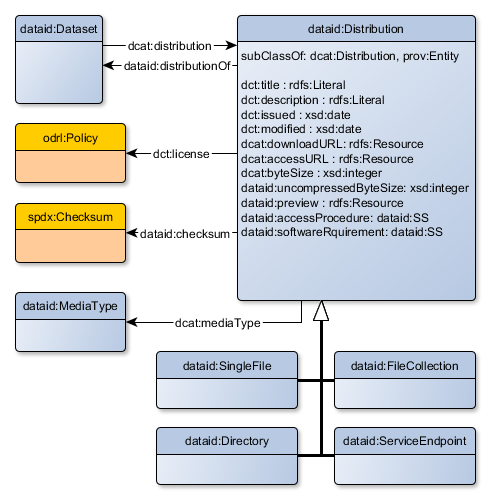
\includegraphics[width=10cm]{images/ClassDistribution.png}
  \caption{Class Distribution}
  \label{fig:example}
\end{figure}

Properties used with \prop{dataid:Distribution}:
\begin{description}
\item[\prop{dcat:mediaType}:] is restricted to a range of \prop{dataid:MediaType} (see next \cref{sec:coremediatype}). This property is absolutely necessary to automatically digest the content of a Distribution. \textbf{(M)}
\item[\prop{dcat:downloadURL}:] this property supplies a URL under which the described Distribution can be downloaded directly (without any access procedure or intermediate steps) and completely. \textbf{(M if no \prop{dcat:accessURL})}
\item[\prop{dcat:accessURL}:] when additional steps are necessary to achieve access to the data of this Distribution (such as authorization, querying or selecting data from a repository), \prop{dcat:accessURL} is used to provide the initial URL. If the process necessary to retrieve the data is not evident by the content of the web page referred, publishers should make use of property. \prop{dataid:accessProcedure}. \textbf{(M if no \prop{dcat:downloadURL})}
\item[\prop{dataid:accessProcedure}:] is used to convey a description of necessary steps, needed to retrieve the data of this Distribution from the \prop{dcat:accessURL}. This property should not be used in connection with \prop{dcat:downloadURL}. \textbf{(R if no \prop{dcat:downloadURL})}
\item[\prop{dataid:checksum}:] the range of this property is restricted to \prop{spdx:Checksum} \cite{spdx}, providing \prop{spdx:checksumValue} and \prop{spdx:algorithm} properties for an exact definition of a checksum. Checksums can be used to validate the correctness of downloaded files, directories and API endpoint responses. \textbf{(R)}
\item[\prop{dcat:byteSize}:] The exact size of a distribution in bytes. \textbf{(R)}
\item[\prop{dataid:softwareRequirement}:] Some data formats/serialisations are only useful with a particular software product. This statement offers the possibility to name such circumstance. \textbf{(O)}
\item[\prop{dataid:uncompressedByteSize}:] Often, files and media streams are compressed to reduce the amount of bytes to be transferred. This optional property provides the means to specify the size of the Distribution in its uncompressed extension. \textbf{(O)}
\item[\prop{dataid:preview}:] While the exact format and serialisation of the Distribution is defined by \prop{dataid:MediaType}, it is often beneficial for publishers and consumers to have a look at the actual format of the (uncompressed) data. This property points out a web resource providing such a preview. \textbf{(O)}
\item[\prop{dataid:distributionOf}:] the inverse property of \prop{dcat:distribution}, pointing back to the Dataset instance this Distribution belongs to. \textbf{(O)}
\item[\prop{dct:license}:] see \cref{sec:coredataset} for a detailed description. Often, the license used for the Distribution is the same as for the pertaining Dataset. For those cases where this is not true, the use of this property in the context of a Distribution is advised. \textbf{(O)}
\end{description}

The first example is an instance of \prop{dataid:SingleFile}, describing a single RDF file (which contains the whole Dataset) in Turtle syntax, compressed with the bzip2 compression. It can be downloaded directly (without any intermediate steps), hence the property \prop{dcat:downloadURL} is used to point out the resource on the Web. Since it is a compressed file, the byte size in its compressed and uncompressed state is provided. An instance of \prop{spdx:Checksum} was included, providing the checksum value for this Distribution.
\\
\begin{lstlisting}[language=ttl, captionpos=b,caption=A single file Distribution,label=lst:coresuperset,linewidth=\columnwidth,breaklines=true]
<dataid_ar.ttl?file=long_abstracts_en_uris_ar.ttl.bz2>
        a                        dataid:SingleFile ;
        dct:license              <http://purl.oclc.org/NET/rdflicense/cc-by-sa3.0> ;                              
        dct:publisher            <http://wiki.dbpedia.org/dbpedia-association> ;
        dataid:associatedAgent   <http://wiki.dbpedia.org/dbpedia-association> ;
        dataid:checksum          <dataid_ar.ttl?file=long_abstracts_en_uris_ar.ttl.bz2&checksum=md5> ;            
        dataid:isDistributionOf  <dataid_ar.ttl?set=long_abstracts_en_uris> ;                                     
        dataid:preview           <http://downloads.dbpedia.org/preview.php?file=2015-10_sl_core-i18n_sl_ar_sl_long_abstracts_en_uris_ar.ttl.bz2> ;.
        dataid:uncompressedByteSize      186573907 ;                                                              
        dcat:byteSize                    33428372 ;                                                               
        dcat:downloadURL         <long_abstracts_en_uris_ar.ttl.bz2> ;                                            
        dcat:mediaType           dataid:MediaType_turtle_x-bzip2                                                  

<dataid_ar.ttl?file=long_abstracts_en_uris_ar.ttl.bz2&checksum=md5>                                               
        a                   spdx:Checksum ;
        spdx:algorithm      spdx:checksumAlgorithm_md5 ;                                                          
        spdx:checksumValue  "2503179cd96452d33becd1e974d6a163"^^xsd:hexBinary .  
\end{lstlisting}

The second example is an instance of \prop{dataid-ld:SparqlEndpoint}, a sub class of \prop{dataid:ServiceEndpoint} and \prop{sd:Service} which was introduced with the DataID extension for Linked Data (dataid-ld). Additional properties from the SPARQL 1.1 Service Description language are used to further describe the endpoint. As opposed to the previous example, this SPARQL endpoint provides multiple Datasets at once in the context of the original \dataid from DBpedia.
\\
\begin{lstlisting}[language=ttl, captionpos=b,caption=Distribution of a SPARQL endpoint,label=lst:coresuperset,linewidth=\columnwidth,breaklines=true]
<dataid_ar.ttl?sparql=DBpediaSparqlEndpoint>
        a                        dataid-ld:SparqlEndpoint ;
        dataid:associatedAgent   <http://support.openlinksw.com/> ;                                               
        dataid:accessProcedure   <dataid_ar.ttl?stmt=sparqlaccproc> ;                                             
        dct:hasVersion           <dataid_ar.ttl?version=1.0> ;
        dct:license              <http://purl.oclc.org/NET/rdflicense/cc-by-sa3.0> ;
        dcat:accessURL           <http://dbpedia.org/sparql> ;                                                    
        dcat:mediaType           <http://dataid.dbpedia.org/ns/mt
        sd:endpoint              <http://dbpedia.org/sparql> ;                                                    
        sd:supportedLanguage     sd:SPARQL11Query ;                                                               
        sd:resultFormat          <http://www.w3.org/ns/formats/RDF_XML>,                                          
            <http://www.w3.org/ns/formats/Turtle> .  
\end{lstlisting}

\subsection{MediaType} 
\label{sec:coremediatype}
\dcat does not offer an intrinsic way of specifying the exact format of the content described by a Distribution. While the property \prop{dcat:mediaType} does exist, its expected range \prop{dct:MediaTypeOrExtend} is an empty concept, not extended by \dcat. Therefore, the \prop{dataid:MediaType} was introduced to better qualify this crucial piece of information. The following properties are of interest:

\begin{description}
\item[\prop{dataid:typeTemplate}:] the IANA media type\footnoteurl{http://www.iana.org/assignments/media-types/media-types.xhtml} - also named mime type \cite{freed1996rfc2046}. This property is of utmost importance for the automatic processing of content. Through its registration with the IANA\footnoteurl{http://www.iana.org}, each type is unambiguously defined and the format of data content can be interpreted in automated processes. \textbf{(M)}
\item[\prop{dataid:typeName}:] name of the described format or serialisation. \textbf{(R)}
\item[\prop{dataid:typeExtension}:] a common file extension for the type described (e.g. '.ttl'). \textbf{(O)}
\item[\prop{dataid:typeReference}:] in some instances, a reference to a useful resource about a type is advisable, to further aid the apprehension of consumer agents (person or software). \textbf{(O)}
\item[\prop{dataid:innerMediaType}:] with this property, descriptions of nested formats become possible (such as a compressed XML file - '.xml.bz2'), useful in pipeline processing. \textbf{(O)}
\end{description}

\begin{figure}[!htbp]
\centering
  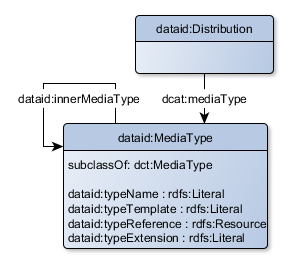
\includegraphics[width=7cm]{images/ClassMediaType.png}
  \caption{Schematic view: A shallow hierarchy of Datasets.}
  \label{fig:example}
\end{figure}

The following extract exemplifies the use of these properties:
\footnote{note: the namespace \url{http://dataid.dbpedia.org/ns/mt#} for common MediaTypes is used on a preliminary basis)}
\\
\begin{lstlisting}[language=ttl, captionpos=b,caption=Example of a complex media type,label=lst:coresuperset,linewidth=\columnwidth,breaklines=true]
<http://dataid.dbpedia.org/ns/mt#MediaType_turtle_x-bzip2>
        a                      dataid:MediaType ;
        dataid:innerMediaType  <http://dataid.dbpedia.org/ns/mt#MediaType_turtle> ;  
        dataid:typeName        "Turtle Bzip2" ;
        dataid:typeExtension   ".bz2" ;  
        dataid:typeTemplate    "application/x-bzip2" 

<http://dataid.dbpedia.org/ns/mt#MediaType_turtle>
        a                     dataid:MediaType ;
        dataid:typeName       "Turtle" ;
        dataid:typeExtension  ".ttl" ;
        dataid:typeTemplate   "application/x-turtle" ;   
        dataid:typeTemplate   "text/turtle" .
\end{lstlisting}

\subsection{Agent} 
\label{sec:coreagent}
An Agent is something or someone that bears some form of responsibility for an Entity or activities which create, transform or manage Entities in some way. Agents are real or legal persons, groups of persons, programs, organisations etc. The class \prop{dataid:Agent} subsumes both agent concepts of \prov and \foaf ontologies, to further incorporate \prov into the context of \dcat (which uses \prop{foaf:Agent} to portray this concept). 

The attributes of the \foaf vocabulary\footnoteurl{http://xmlns.com/foaf/spec/} are used to describe aspects such as name and e-mail address of a person. In addition, the following properties were introduced in \core:

\begin{description}
\item[\prop{dataid:hasAuthorization}:] the inverse property of \prop{dataid:authorizedAgent}, pointing out an Authorization which grants an Agent some kind some authority over Entities. This is explained in detail in the example on Authorizations in the next \cref{sec:coreauthorization}. \textbf{(R)}
\item[\prop{dataid:identifier}:] often, Agents have already unique identifiers somewhere on the Web (in addition to the URI used in the context of a \dataid document, such as URI, ORCID\footnoteurl{http://orcid.org} or researcherId\footnoteurl{http://www.researcherid.com}). This property points out additional identifiers (see \cref{sec:coreidentifier}). \textbf{(O)}
\end{description}

\begin{figure}[!htbp]
\centering
  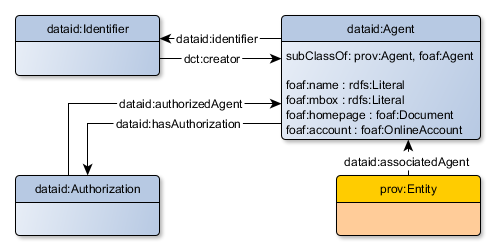
\includegraphics[width=10cm]{images/ClassAgent.png}
  \caption{Schematic view: A shallow hierarchy of Datasets.}
  \label{fig:example}
\end{figure}

This example of an Agent portrays the DBpedia association\footnoteurl{http://wiki.dbpedia.org/dbpedia-association}:
\\
\begin{lstlisting}[language=ttl, captionpos=b,caption=Example of an organisation,label=lst:coresuperset,linewidth=\columnwidth,breaklines=true]
<http://wiki.dbpedia.org/dbpedia-association>
        a                        dataid:Agent ;
        dataid:hasAuthorization  <dataid_ar.ttl?auth=creatorAuthorization> ; 
        foaf:homepage            <http://dbpedia.org> ;
        foaf:mbox                "dbpedia@infai.org" ;                                                        
        foaf:name                "DBpedia Association" .
\end{lstlisting}

\subsection{Authorization} 
\label{sec:coreauthorization}
One objective of \core is the detailed expression of the relations between Agents and Entities. To qualify these relations (summarised under the property \prop{dataid:associatedAgent}) AgentRoles have to be assigned to the involved Agents (such as Maintainer, Publisher etc.). This is achieved by the class \prop{dataid:Authorization}, which is a sub class of \prop{prov:Attribution}, a qualification of the property \prop{prov:wasAttributedTo}. It basically states, which AgentRole(s) (pointed out with \prop{dataid:authorityAgentRole}) an Agent (via \prop{dataid:authorizedAgent}) has, regarding a certain collection of Entities (\prop{dataid:authorizedFor}). This mediator is further qualified by an optional period of time for which it is valid and access restrictions by the Entities themselves, allowing only specific Authorizations to exert influence over them (see \prop{dataid:needsSpecialAuthorization}). 

\Cref{chap:bestprctice} contains a detailed example on Authorizations, to deepen the understanding of this concept as well as to provide suitable use cases.

\begin{figure}[!htbp]
\centering
  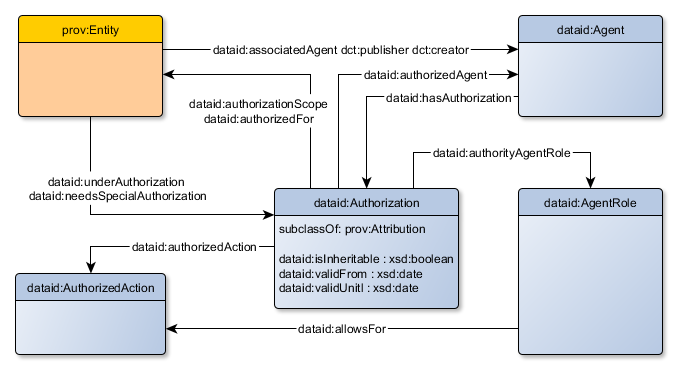
\includegraphics[width=\textwidth]{images/ClassAuthorization.png}
  \caption{Schematic view: A shallow hierarchy of Datasets.}
  \label{fig:example}
\end{figure}

\begin{description}
\item[\prop{dataid:authorizedAgent}:] each Authorization shall have at least on associated Agent, which are pointed out via this property (sub property of \prop{prov:agent}). \textbf{(M)}
\item[\prop{dataid:authorityAgentRole}:] provides the AgentRole the Agent(s) of this Authorization are assigned with (sub property of \prop{prov:hadRole}). \textbf{(M)}
\item[\prop{dataid:authorizedFor}:] this property points out those Entities for which this Authorization is valid (sub property of \prop{dataid:authorizationScope}). \textbf{(M)}
\item[\prop{dataid:authorizedAction}:] an AgentRole entails the right (or responsibility) for Agents to execute a collection of defined AuthorizedAction(s). This property can be inferred by a chain of properties (OWL property chain axiom): \prop{dataid:authorityAgentRole} / \prop{dataid:allowsFor}. \textbf{(O)}
\item[\prop{dataid:isInheritable}:] indicates whether an Authorization is transferable when changing versions of a \dataid. Thus, keeping Agent, AgentRole and Actions in place for the updated versions of all involved Entities. \textbf{(O)}
\item[\prop{dataid:validFrom}:] defining the temporal beginning (inclusive) of an Authorization (the time from which on out the axioms of an Authorization are valid). \textbf{(O)}
\item[\prop{dataid:validUntil}:] defining the temporal ending (exclusive) of an Authorization (the time from which on out the axioms of an Authorization are no longer valid). \textbf{(O)}
\end{description}

The property \prop{dataid:authorizationScope} is an abstract super property of \prop{dataid:authorizedFor}, pointing to all referred and inferred Entities which are under a certain Authorization. Triples with this predicate are inferred by its sub properties \prop{dataid:authorizedFor} and the virtual properties \prop{dataid:authorizationChain1} to \prop{dataid:authorizationChain9}. An exact explanation of Authorizations and all involved properties is accompanying the extended example on Authorizations at the end of this chapter (see \cref{sec:exauthorization}).

Furthermore, property \prop{dataid:underAuthorization} is the inverse of \prop{dataid:authorizationScope} and a sub property of \prop{prov:wasAttributedTo}, pointing out the qualification instance which qualifies the relation \prop{dataid:associatedAgent}. Its sub property \prop{dataid:needsSpecialAuthorization} was introduced to restrict the reach of Authorizations, to the exclusion of those Authorizations, not referenced via this property (or simply: if an Entity has a \prop{dataid:needsSpecialAuthorization} instance, all Authorizations without this referral are impotent).

The following snippet provides a simple example of two AgentRoles being assigned to two Agents for a DataId instance (and thereby for every Entity involved in this \dataid  - see \cref{chap:bestprctice} for more).
\\
\begin{lstlisting}[language=ttl, captionpos=b,caption=Example of an organisation,label=lst:coresuperset,linewidth=\columnwidth,breaklines=true]
<http://wiki.dbpedia.org/dbpedia-association/persons/Freudenberg>
        a                        dataid:Agent ;                                               
        dataid:hasAuthorization  <dataid_ar.ttl?auth=maintainerAuthorization> ;
        foaf:mbox                "freudenberg@informatik.uni-leipzig.de" ;
        foaf:name                "Markus Freudenberg"                     ;
        dataid:identifier        <http://www.researcherid.com/rid/L-2180-2016> .              

<dataid_ar.ttl?auth=maintainerAuthorization>
        a                          dataid:Authorization ;                                     
        dataid:authorityAgentRole  dataid:Maintainer ;                                        
        dataid:authorizedAgent     <http://wiki.dbpedia.org/dbpedia-association/persons/Freudenberg> ;
        dataid:authorizedFor       <dataid_ar.ttl> .                                          

<http://wiki.dbpedia.org/dbpedia-association>
        a                        dataid:Agent ;                                               
        dataid:hasAuthorization  <dataid_ar.ttl?auth=creatorAuthorization> ;
        foaf:homepage            <http://dbpedia.org> ;
        foaf:mbox                "dbpedia@infai.org" ;
        foaf:name                "DBpedia Association" .

<dataid_ar.ttl?auth=creatorAuthorization>
        a                          dataid:Authorization ;
        dataid:authorityAgentRole  dataid:Creator ;                                           
        dataid:authorizedAgent     <http://wiki.dbpedia.org/dbpedia-association> ;
        dataid:authorizedFor       <dataid_ar.ttl> .
\end{lstlisting}

\subsection{AuthorizedAction \& AgentRole} 
\label{sec:coreaction}
The AgentRole assigned to an Agent in the context of an \prop{dataid:Authorization} is defined only by the property \prop{dataid:allowsFor}, pointing out AuthorizedActions it entails. A \prop{dataid:AuthorizedAction} shall either be a dataid:EntitledAction, representing all AuthorizedActions an Agent could take, or the AuthorizedActions an Agent has to take (\prop{dataid:ResponsibleAction}). 

\begin{figure}[!htbp]
\centering
  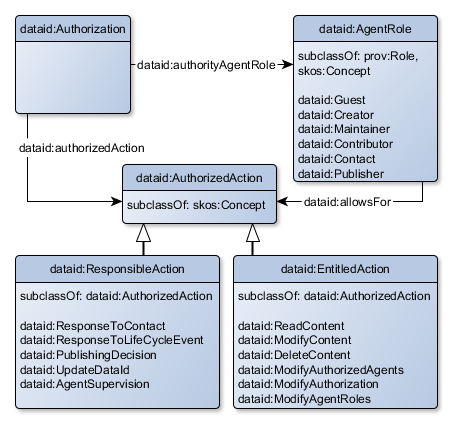
\includegraphics[width=9cm]{images/ClassAuthorizedAction.png}
  \caption{Schematic view: A shallow hierarchy of Datasets.}
  \label{fig:example}
\end{figure}

AuthorizedActions and AgentRoles defined in this ontology are only examples of possible implementations, reflecting a common environment of a File or Document Management System. They can be replaced to fit the use case at hand. Implementing them as a \prop{skos:ConceptScheme}\footnoteurl{https://www.w3.org/TR/skos-reference/#ConceptScheme} offers additional semantics, for example in determining which AgentRole can override AuthorizedActions initiated by Agents with other AgentRoles for the same Entity. The following descriptions will shortly introduce each individual, predefined in the \core ontology.

{\large\textbf{Agent Roles:}}
\begin{description}
\item[Creator:] Creator of the resource. An AgentRole that is credited with the main part in the initial creation of the resource.
\item[Contact:] An Agent that can be contacted for general requests about the resource.
\item[Contributor:] Contributor to the resource. An Agent that was involved in creating or maintaining the resource but does not have the main part in this activity.
\item[Guest:] A visitor or anonymous Agent has only read rights on public documents.
\item[Maintainer:] Maintainer of the Dataset. An Agent that ensures the technical correctness, accessibility and up-to-dateness of a Dataset.
\item[Publisher:] Publisher of the Dataset. An Agent that makes the Dataset accessible online on a server or repository without necessarily being involved in its creation.\\
\end{description}

{\large\textbf{Responsible Actions:}}
\begin{description}
\item[ResponseToContact:] The responsibility to respond to contact attempts by external Agents. A contact point for the Entity.
\item[ResponseToLifeCycleEvent:] The responsibility to manage changes and react to bugs and issues that are reported concerning a Dataset.
\item[PublishingDecision:] The responsibility to decide if an Entity should be published.
\item[UpdateDataId:] The responsibility to update dataset metadata.
\item[AgentSupervision:] The responsibility to supervise other Agents.\\
\end{description}

{\large\textbf{Entitled Actions:}}
\begin{description}
\item[ReadDataId:] read the DataID dataset metadata.
\item[ReadContent:] read the content of an Entity.
\item[ModifyContent:] modify the content of an Entity.
\item[DeleteContent:] delete some content of an entity.
\item[ModifyAuthorizedAgents:] modify which Agents are authorized on certain Entities.
\item[ModifyAuthorization:] modify an Authorization.
\item[ModifyAgentRoles:] modify the role of Agents on certain Entities.
\end{description}

This example is not part of the running example, but has been lent from the \core ontology document itself. Here the AgentRole 'Contact' is defined in the context of a \prop{skos:ConceptScheme}.
\\
\begin{lstlisting}[language=ttl, captionpos=b,caption=Example of an organisation,label=lst:coresuperset,linewidth=\columnwidth,breaklines=true]
dataid:Contact
	a owl:NamedIndividual, dataid:AgentRole;
	rdfs:isDefinedBy <http://dataid.dbpedia.org/ns/core#> ;
	dataid:allowsFor dataid:ReadDataId; 
	dataid:allowsFor dataid:ModifyContent;
	dataid:allowsFor dataid:ReadContent;
	dataid:allowsFor dataid:ResponseToContact;
        rdfs:comment "Contact agent. An agent that can be contacted for general requests about the resource."@en ;
        skos:prefLabel "contact"@en ;
	skos:inScheme dataid:AgentRoleScheme ; 
	skos:broader dataid:Publisher, dataid:Maintainer .   
\end{lstlisting}

\subsection{DatasetRelationship} 
\label{sec:corerelation}
A DatasetRelationship is a qualification of the generic property \prop{dataid:relatedDataset} (which is a sub-property of \prop{dct:relation}). The \prop{dataid:DatasetRelationship} is a subclass of \prop{prov:EntityInfluence} and is defined by three properties:

\begin{description}
\item[\prop{dataid:datasetRelationRole}:] specifying the role (or type) of this relationship, defining the exact role the 'target' Dataset takes in regard to the 'origin' dataset of this relationship.
\item[\prop{dataid:qualifiedRelationOf}:] the inverse property of \prop{qualifiedDatasetRelation} is pointing out the origin Dataset of this qualification.
\item[\prop{dataid:qualifiedRelationTo}:] the target Dataset of this qualification.
\end{description}

\begin{figure}[!htbp]
\centering
  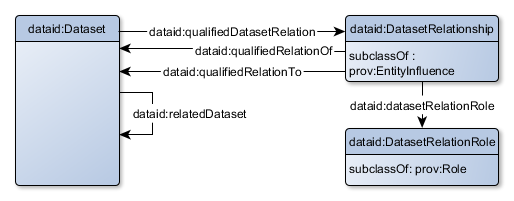
\includegraphics[width=10cm]{images/ClassDatasetRelationship.png}
  \caption{Schematic view: A shallow hierarchy of Datasets.}
  \label{fig:example}
\end{figure}

The class \prop{dataid:DatasetRelationRole} is not further qualified in the context of \core, which could be done in an extension to \core, similar to \prop{dataid:AgentRole}. Some instances of this class are already provided:

\begin{description}
\item[GenericRelation:] specifies a \prop{dataid:DatasetRelationship} between two datasets which have a relation of a unknown quality (such a relation is equivalent to direct \prop{dct:relation} property).
\item[DerivatRole:] specifies a \prop{dataid:DatasetRelationship} where one dataset points out a second dataset, which is a derivat of the first.
\item[SourceRole:] specifies a \prop{dataid:DatasetRelationship} where the origin dataset is created by transforming/collecting data from the target dataset.
\item[CopyRole:] specifies a \prop{dataid:DatasetRelationship} where the origin dataset is an exact copy of the target dataset (e.g. when republished under a different domain).
\item[SimilarityRole:] specifies a \prop{dataid:DatasetRelationship} where the origin dataset has a significant similarity to the target dataset (without any assertion as to dimension of similarity).
\end{description}

In the example, the Wikipedia source dataset (named 'pages\_articles') of a given DBpedia dataset is referred to with the help of this concept:
\\
\begin{lstlisting}[language=ttl, captionpos=b,caption=Example of an organisation,label=lst:coresuperset,linewidth=\columnwidth,breaklines=true]
<dataid_ar.ttl?relation=source&target=pages_articles>
        a                           dataid:DatasetRelationship ;
        dataid:datasetRelationRole  dataid:SourceRole ;
        dataid:qualifiedRelationOf  <dataid_ar.ttl?set=long_abstracts_en_uris> ;
        dataid:qualifiedRelationTo  <dataid_ar.ttl?set=pages_articles> .  
\end{lstlisting}

\subsection{Identifier} 
\label{sec:coreidentifier}
The class \prop{dataid:Identifier} uniquely identifies any resource (incl. Entities and Agents), given an identifier as a literal and a corresponding \prop{datacite:IdentifierScheme} (e.g. ORCID, ResearcherID etc.). Typically an organisation is responsible for issuing and managing Identifiers described with this concept, which can be referred to with \prop{dct:creator}. \core adopted this approach from Datacite ontology (see \cref{sec:datacite}) to provide a schematic way of adding additional, existing identifiers to Entities and Agents referenced in a \dataid document.
\todo{add something about refining the datacite ontology}
\begin{figure}[!htbp]
\centering
  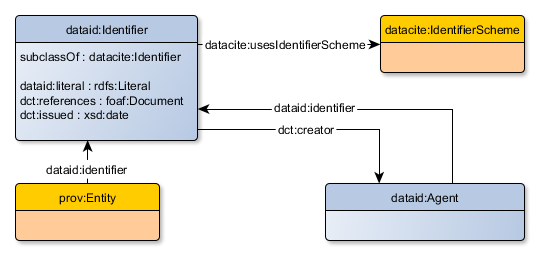
\includegraphics[width=10cm]{images/ClassIdentifier.png}
  \caption{Schematic view: A shallow hierarchy of Datasets.}
  \label{fig:example}
\end{figure}

\begin{description}
\item[\prop{dataid:literal}:] the identifier as literal (e.g. a URI as literal). \textbf{(M)}
\item[\prop{datacite:usesIdentifierScheme}:] an IdentifierScheme defines (among other attributes) a pattern against which the literal of an identifier is validated. Thereby the validity of an identifier is tested. \textbf{(M)}
\item[\prop{dct:references}:] often identifier agencies have web presentations for their identifiers (e.g. ORCID\footnoteurl{http://orcid.org/0000-0002-1825-0097}). Such a website can be referenced with this property. \textbf{(O)}
\item[\prop{dct:creator}:] can be used to identify the identifier agency, responsible for an identifier and pertaining scheme. \textbf{(O)}
\end{description}

\begin{lstlisting}[language=ttl, captionpos=b,caption=Example of an organisation,label=lst:coresuperset,linewidth=\columnwidth,breaklines=true]
<http://www.researcherid.com/rid/L-2180-2016>
        a                              dataid:Identifier ;
        dataid:literal                 "L-2180-2016" ;                                        
        dct:issued                     "2016-08-01"^^xsd:date ;
        dct:references                 <http://www.researcherid.com/rid/L-2180-2016> ;        
        datacite:usesIdentifierScheme  datacite:researcherid .  
\end{lstlisting}

\subsection{SimpleStatement} 
\label{sec:corestatement}
The concept dataid:SimpleStatement is intended as a tool for conveying a statement, definition or point of view about a certain topic. Using either a simple literal (using \prop{dataid:literal}) to provide a quotation or by a referencing a web resource providing or representing the statement in any medium (picture, text, video etc.). This class is a sub class of \prop{prov:Entity} and implements in addition the following Dublin Core classes: \prop{dct:ProvenanceStatement}, 
\prop{dct:RightsStatement},
\prop{dct:Standard}
. With this measure, it is possible to attach provenance information onto instances of this concept and to use \prop{dataid:SimpleStatement} as range of \prop{dct:rights} and its sub-properties, \prop{dct:provenance}, \prop{dct:conformsTo} and others.

This reification approach with an intermediate resource was chosen to cover as many scenarios as possible including many edge cases which do not have to be modelled explicitly. To provide a minimum of structure for textual statements, as well as providing an resource onto which provenance information could be it easy to attach provenance information to a statement. 

\begin{figure}[!htbp]
\centering
  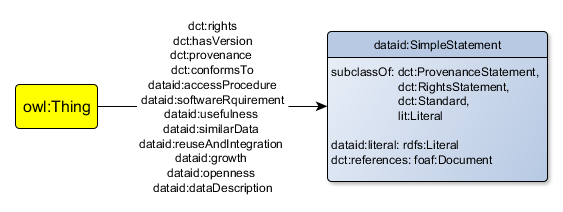
\includegraphics[width=10cm]{images/ClassSimpleStatement.png}
  \caption{Schematic view: A shallow hierarchy of Datasets.}
  \label{fig:example}
\end{figure}

\begin{description}
\item[\prop{dataid:literal}:] a textual statement 'from humans for humans'. \textbf{(R)}
\item[\prop{dct:references}:] the alternative reference to a web resource containing the human readable statement. \textbf{(O)}
\end{description}

Two instances from the running example demonstrating the different usage scenarios of this concept. The first is the official rights statement of the DBpedia association, while the second is the access procedure for the DBpedia SPARQL endpoint, where \prop{dct:reference} is pointing out the SPARQL 1.1 specification (as a web page specifying the means of querying the endpoint).\todo{define SPARQL somewhere}
\\
\begin{lstlisting}[language=ttl, captionpos=b,caption=Example of an organisation,label=lst:coresuperset,linewidth=\columnwidth,breaklines=true]
<dataid_ar.ttl?rights=dbpedia-rights>
        a                 dataid:SimpleStatement ;                                            
        dataid:literal  """DBpedia is derived from Wikipedia and is distributed under the same licensing terms as Wikipedia itself. As Wikipedia has moved to dual-licensing, we also dual-license DBpedia starting with release 3.4. Data comprising DBpedia release 3.4 and subsequent releases is licensed under the terms of the Creative Commons Attribution-ShareAlike 3.0 license and the GNU Free Documentation License. Data comprising DBpedia releases up to and including release 3.3 is licensed only under the terms of the GNU Free Documentation License."""@en .

<dataid_ar.ttl?stmt=sparqlaccproc>
        a                 dataid:SimpleStatement ;                                            
        dct:references    <https://www.w3.org/TR/sparql11-overview/> ;                        
        dataid:literal  "An endpoint for sparql queries: provide valid queries."@en .
\end{lstlisting}

\section{Complex Example on Authorizations} 
\label{sec:exauthorization}

I decided to provide a more prolific example on the subject of Authorizations, since this concept is of more complex nature. In particular, the impact of \prop{dataid:authorizationScope} with its sub-properties is difficult to understand at first sight.

The property \prop{dataid:authorizationScope} has the role of an abstract super property, pointing out all referred and inferred Entities under a given Authorization and is usually not instantiated in a \dataid graph. It can be inferred directly by the existence of  \prop{dataid:authorizedFor}, which is used to reference Entities to which an Authorization applies and all its rules and restrictions are tailored for.

The following axioms for the transitive property \prop{dataid:authorizationScope} would be desirable to extend the influence of an Authorization along any property path combined of \prop{foaf:primaryTopic}, \prop{void:subset} and \prop{dcat:distribution}, initiated by an instance of \prop{dataid:authorizedFor}.

{\footnotesize
\vspace*{-0.5cm}
\begin{align*}
foaf:primaryTopic \sqsubseteq dataid:authorizationScope\\
void:subset \sqsubseteq dataid:authorizationScope\\
dcat:distribution \sqsubseteq dataid:authorizationScope\\
dataid:authorizedFor \sqsubseteq dataid:authorizationScope
\end{align*}
}%
To not hijack foreign ontologies \cite{feeney2015linked} (e.a. \dcat, \void or \foaf), a series of properties (\prop{dataid:authorisationChain1} - \prop{dataid:authorisationChain9}) were introduced to simulate this behaviour with the help of the OWL property chain axiom\todo{needs link}. 

Properties \prop{dataid:authorisationChain1} to \prop{dataid:authorisationChain6}:

{\footnotesize
\vspace*{-0.5cm}
\begin{align*}
foaf:primaryTopic \circ dcat:distribution \sqsubseteq dataid:authorizationScope\\
foaf:primaryTopic \circ void:subset \sqsubseteq dataid:authorizationScope\\
void:subset \circ dcat:distribution \sqsubseteq dataid:authorizationScope\\
void:subset \circ void:subset \sqsubseteq dataid:authorizationScope\\
void:subset \circ void:subset \circ dcat:distribution \sqsubseteq dataid:authorizationScope\\
foaf:primaryTopic \circ void:subset \circ dcat:distribution \sqsubseteq dataid:authorizationScope
\end{align*}
}%
With these properties all subsequent Entities connected to the origin Entity (the Entity referenced from an Authorization with \prop{dataid:authorizedFor}), are under the influence of this Authorization, connected with it via the transitive \prop{dataid:authorizationScope}. One exception remains: those Entities second in line after the origin Entity are skipped in this progression.
Properties \prop{dataid:authorisationChain7} to \prop{dataid:authorisationChain9} are solving this issue:

{\footnotesize
\vspace*{-0.5cm}
\begin{align*}
dataid:authorizedFor \circ foaf:primaryTopic \sqsubseteq dataid:authorizationScope\\
dataid:authorizedFor \circ void:subset \sqsubseteq dataid:authorizationScope\\
dataid:authorizedFor \circ dcat:distribution \sqsubseteq dataid:authorizationScope
\end{align*}
}%
For example: if a knowledge base (KB) holds some statements, such as:
\begin{lstlisting}[language=ttl, captionpos=b,label=lst:coresuperset,linewidth=\columnwidth,breaklines=true]
ex:someAuthorization	dataid:authorizedFor		ex:DataId .
ex:DataId		foaf:primaryTopic		ex:RootDataset .
ex:RootDataset		void:subset			ex:DatasetC . 
\end{lstlisting}

we can infer the following statements:
\begin{lstlisting}[language=ttl, captionpos=b,label=lst:coresuperset,linewidth=\columnwidth,breaklines=true]
ex:someAuthorization 	dataid:authorizationScope 	ex:DataId .
ex:someAuthorization 	dataid:authorizationScope 	ex:RootDataset .
ex:someAuthorization 	dataid:authorizationScope 	ex:DatasetC . 
\end{lstlisting}

by inferring these statements first:	
\begin{lstlisting}[language=ttl, captionpos=b,label=lst:coresuperset,linewidth=\columnwidth,breaklines=true]
ex:DataId 		dataid:authorizationChain2 	ex:DatasetC .
ex:DataId	 	dataid:authorizationChain6 	ex:DistributionC1 .
ex:someAuthorization 	dataid:authorizationChain7 	ex:RootDataset .
\end{lstlisting}

With these auxiliary properties the inference of \prop{dataid:authorizationScope} along the depicted property paths becomes feasible:


\begin{figure}[!htbp]
\centering
  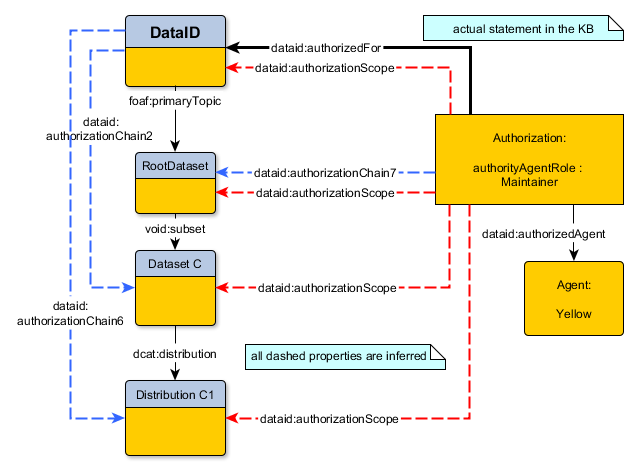
\includegraphics[width=12cm]{images/AuthorizationExample.png}
  %\caption{Schematic view: A shallow hierarchy of Datasets.}
  \label{fig:dlaxioms}
\end{figure}

Here the Authorization for Agent Yellow is not only valid for the \dataid entity, referred to via \prop{dataid:authorizedFor}. By inferring additional statements of this kind, the scope of this Authorization is extended to every Dataset and Distribution connected via \prop{foaf:primaryTopic}, \prop{dcat:distribution} and \prop{void:subset}. By this means, extending the influence (or scope) of an Authorization over multiple Entities without having to point out all of them with \prop{dataid:authorizedFor} is realised, without changing the definitions of the external properties involved, or an inclusion of rule-based axioms (such as SWRL\footnoteurl{https://www.w3.org/Submission/SWRL/}).

The automatic extension of an Authorization has also its drawbacks. By introducing multiple Authorizations in the context of a \dataid document, providing the same AgentRole for an Entity, the author can encounter unintended behaviours. In this example the previous context is enriched by introducing an additional Agent Blue:

\begin{figure}[!htbp]
\centering
  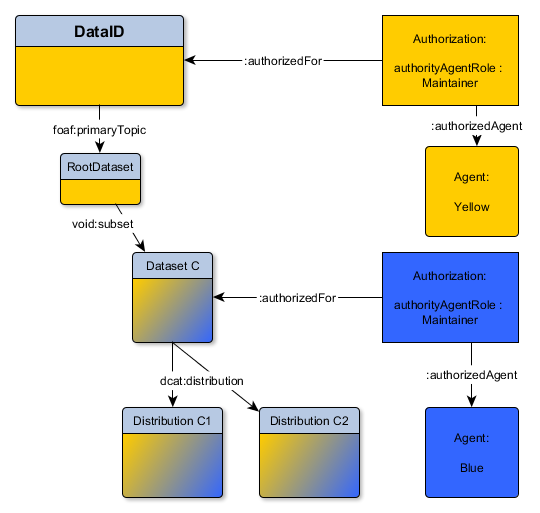
\includegraphics[width=10cm]{images/AuthorizationExample2.png}
  %\caption{Schematic view: A shallow hierarchy of Datasets.}
  \label{fig:dlaxioms}
\end{figure}

DatasetC (and all its Distributions) has two Maintainers, both equally permitted to wield AuthorizedActions as defined by the definition of \prop{dataid:Maintainer}. This behaviour may or may not be intended by the author. To provide the means for restricting Entities to specific Authorizations, the property \prop{dataid:needsSpecialAuthorization} was introduced. This sub-property of \prop{dataid:underAuthorization} (the inverse of \prop{dataid:authorizationScope}) allows to point out those Authorizations with sufficient importance to exert their authority over an Entity, to the exclusion of other Authorizations referenced via \prop{dataid:authorizationScope}.

The following example again expands the already known scenario, by introducing a third Authorization for Agent Green:

\begin{figure}[!htbp]
\centering
  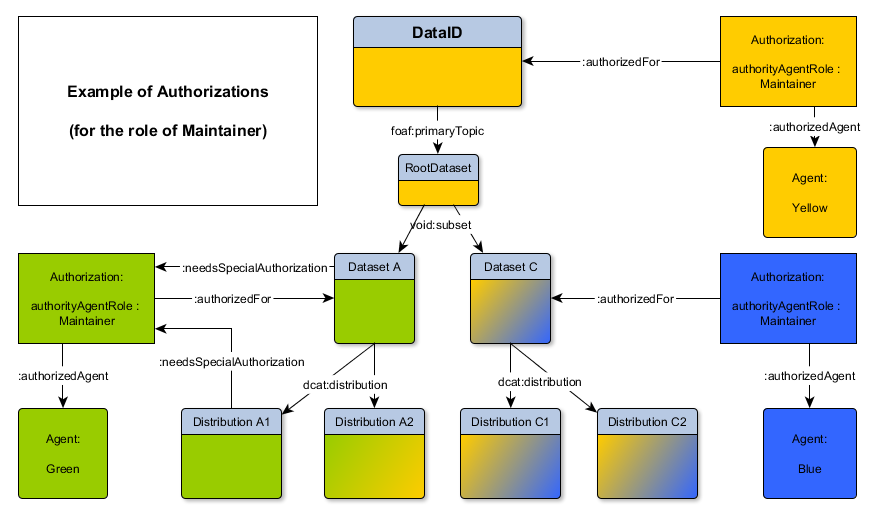
\includegraphics[width=\textwidth]{images/AuthorizationExample5.png}
  %\caption{Schematic view: A shallow hierarchy of Datasets.}
  \label{fig:dlaxioms}
\end{figure}

While DatasetA and DistributionsA1 and A2 are under the Authorizations of Agent Yellow and Agent Green, only DistributionA2 will be maintained by both Agents. DatasetA and DistributionA1 require specifically the Authorization of Agent Green for the purpose of providing the AgentRole of Maintainer.

This mechanism is useful when introducing different levels of privacy into the domain of, for example, a Document Management System (DMS). Two groups of users are specified: The first group (yellow group) should only be able to read the content of a given collection of documents, while the second group (blue group) is also allowed to modify these documents. Therefore, defining two new AgentRoles is advisable. AgentRole 'Reader' can only read the content of Entities available to it, while the 'Editor' allows also for modifying the content. These AgentRoles are linked to via \prop{dataid:authorityAgentRole} from the respective Authorizations of the two groups (\prop{dataid:authorizedAgent} points out the members of a group).

\begin{figure}[!htbp]
\centering
  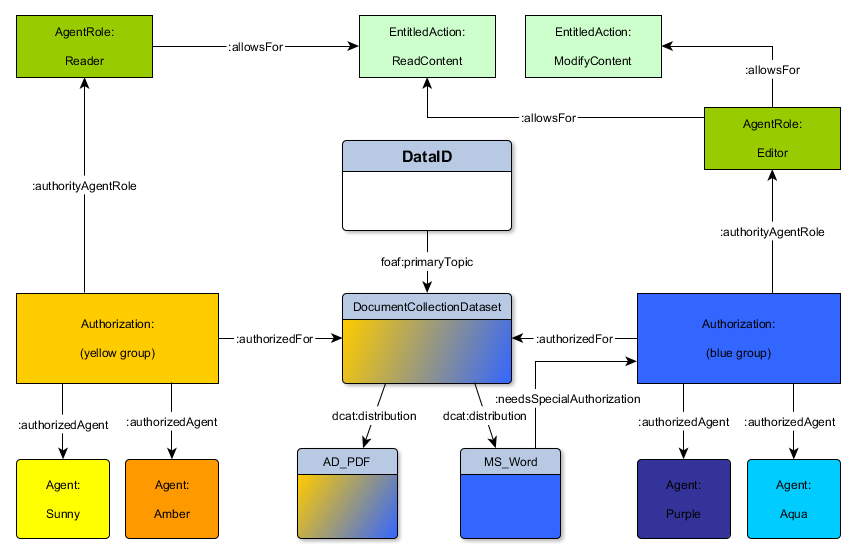
\includegraphics[width=\textwidth]{images/DmsExample.png}
  %\caption{Schematic view: A shallow hierarchy of Datasets.}
  \label{fig:dlaxioms}
\end{figure}

Both Authorizations are authorised for the same document collection (Dataset) and its Distributions as PDF and MS\_Word versions of the same content in the DMS. Since the MS\_Word version of the documents is used for editing the content, while its PDF counterpart is the publishing version, it is sensible to allow only the Editors (blue group) access to the MS\_Word Distribution by using \prop{dataid:needsSpecialAuthorization}. 

\chapter{Publishing Data with DataID}
\label{chap:bestprctice}

\section{Best Practices} 
\label{sec:bestprctice}
Best practices on any kind of methodology or problem have become a ubiquitous companion in our daily life. Be it a Ted Talk\footnoteurl{https://www.ted.com} on how to live to be 100\footnoteurl{https://www.ted.com/talks/dan_buettner_how_to_live_to_be_100} or how to use the Heisenberg Uncertainty Principle in relation to position and momentum\footnoteurl{http://www.dummies.com/education/science/quantum-physics/how-to-use-the-heisenberg-uncertainty-principle-in-relation-to-position-and-momentum/}.

Astonishingly, when it comes to publishing data in a widely accepted manner, only a hand full of comprehensive best practices exist. Most of these best practices, workflows or checklists are further constricted to a certain filed of research, methodology or data type. For example;

\begin{description}
\item[Methodological Guidelines for Publishing
Government Linked Data] "[...] a preliminary set of methodological guidelines for generating, publishing and exploiting Linked Government Data" \cite{Terrazas}
\item[Best Practices for Publishing Linked Data] "[...] a series of best practices designed to facilitate development and delivery of open government data as Linked Open Data." \cite{Hyland:14:BPP}
\item[Key components of data publishing] "From an assessment of the current data-publishing landscape, we highlight important gaps and challenges to consider, especially when dealing with more complex workflows and their integration into wider community frameworks." \cite{austin_2015_34542}
\item[] \todo{add one more}
\end{description}

There are two not quiet distinct categories of best practices on data publishing. 

\paragraph{Workflows} introduce a specific order of activities, the flow of artefacts between them as well as agents and their roles in these processes. Workflows are often summarised in so called Data Lifecycles (or Data Engineering Lifecycle).

The LOD2 Lifeycle of Linked Data \cite{AuerBDEHILMMNSTW12} - used by the ALIGNED project (see \cref{fig:aligned}) - is an portrayal of such a workflow in a domain specific environment.

\begin{figure}[!htbp]
\centering
  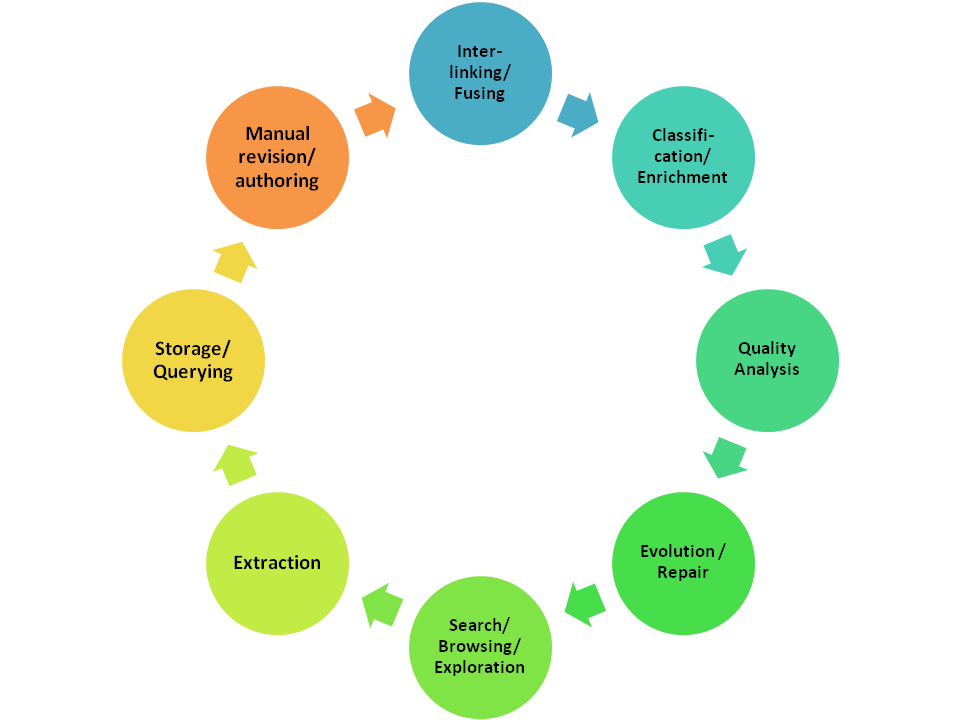
\includegraphics[width=12cm]{images/lod2lifecycle.png}
  \caption{The LOD2 Lifecycle of Linked Data \cite{AuerBDEHILMMNSTW12}}
  \label{fig:lod2lifecycle}
\end{figure}

Many depiction of Data Engineering Lifecycles have domain-independent similarities.
Villaz\'{o}n-Terrazas et al. presented a more generalized version of such a cycle, which I am going to adopt in the context of this work.

 \begin{figure}[!htbp]
\centering
  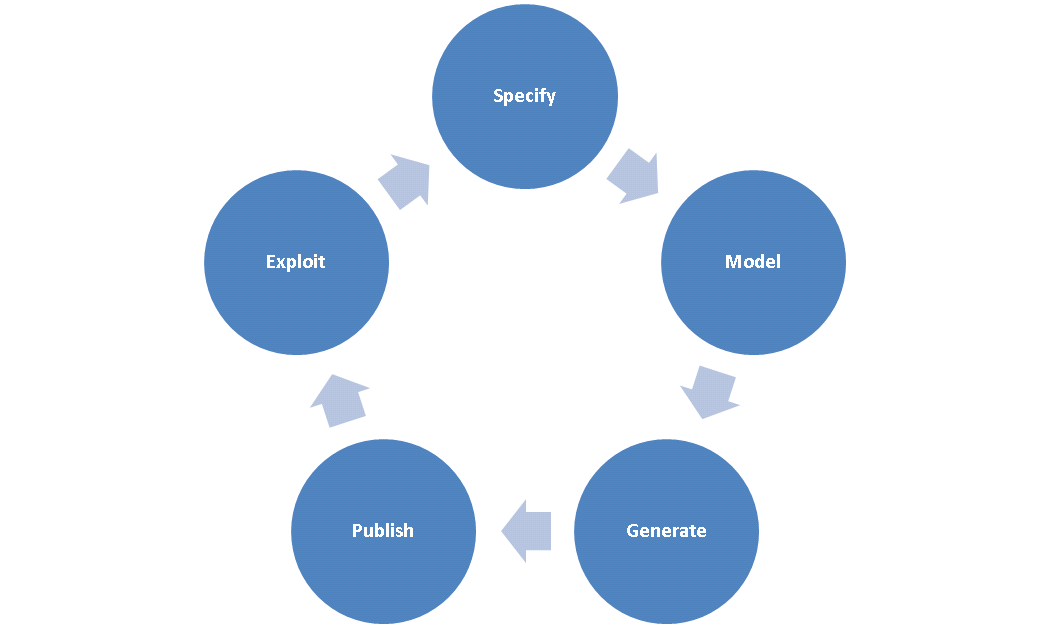
\includegraphics[width=9cm]{images/Villazon-terrazas.png}
  \caption{The Government Linked Data Lifecycle \cite{Terrazas}}
  \label{fig:gldlifecycle}
\end{figure}

A concise summary, tracing the bubble graph above:

\begin{itemize}
\item Specify
\begin{itemize}
\item analysis of data sources (which data (slices) are useful) or previous version of the dataset
\item Select/Design Identifier scheme user to identify records
\end{itemize}
\item Model
\begin{itemize}
\item search/create suitable schema/vocabulary on which to base the datasets
\end{itemize}
\item Generate
\begin{itemize}
\item transform the data sources
\item clean (and validate) the result
\end{itemize}
\item Publish
\begin{itemize}
\item improve discoverability (choose suitable data portal, announce release at different venues)
\item publish the created datasets
\item publish the pertaining metadata
\end{itemize}
\item Exploit
\begin{itemize}
\item different consumer side activities (browsing, integrating, analysing etc.)
\item collect feedback from consumers, improve data
\end{itemize}
\end{itemize}

\paragraph{Checklists} are collections of general advises, how-tos and precautions on publishing data without a particular ordering of items. 

The most comprehensive collection of best practices about publishing data has emerged with the establishment  
of the 'Data on the Web' W3C Working Group\footnoteurl{https://www.w3.org/2013/dwbp/wiki/Main_Page} and their best practices document \cite{dwbpW3C2016} (released as recommendation candidate by the time of writing). 

%Besides the set of best practices, a list of benefits for publishing data on the Web is presented in this document

This set of recommendations touches upon most of the crucial issues when publishing data (with the noted exception of dissemination tasks). I endorse these 35 best practices to their full extend and recommend following all of the suggestions made. Datasets published with adhering to the suggestions made would reap all benefits towards which these best practices were aimed: \textit{Reuse, Comprehention, Linkability, Discoverabilty, Trust, Access, Interoperability and Processability}.\todo{check phrasing}

In this chapter I want to build on this foundation, by expanding on metadata composition and deployment with \dataid (\cref{sec:composingmetadata}). In addition, I want to contribute to the discussion on publishing data, with a specialised checklist \todo{specialised?} for publishing Linked Data datasets (\cref{sec:checklist}), based on the experiences I have accumulated when publishing official DBpedia releases.

\iffalse
\begin{description}
\item[1. Provide metadata] Provide metadata for both human users and computer applications.
\item[2. Provide descriptive metadata] Provide metadata that describes the overall features of datasets and distributions.
\item[3. Provide structural metadata] Provide metadata that describes the schema and internal structure of a distribution.
\item[4. Provide data license information] Provide a link to or copy of the license agreement that controls use of the data.
\item[5. Provide data provenance information] Provide complete information about the origins of the data and any changes you have made.
\item[6. Provide data quality information] Provide information about data quality and fitness for particular purposes.
\item[7. Provide a version indicator] Assign and indicate a version number or date for each dataset.
\item[8. Provide version history] Provide a complete version history that explains the changes made in each version.
\item[9. Use persistent URIs as identifiers of datasets] Identify each dataset by a carefully chosen, persistent URI. 
\item[10. Use persistent URIs as identifiers within datasets] Reuse other people's URIs as identifiers within datasets where possible.
\item[11. Assign URIs to dataset versions and series] Assign URIs to individual versions of datasets as well as to the overall series.
\item[12. Use machine-readable standardized data formats] Make data available in a machine-readable, standardized data format that is well suited to its intended or potential use.
\item[13. Use locale-neutral data representations] Use locale-neutral data structures and values, or, where that is not possible, provide metadata about the locale used by data values.
\item[14. Provide data in multiple formats] Make data available in multiple formats when more than one format suits its intended or potential use.
\item[15. Reuse vocabularies, preferably standardized ones] Use terms from shared vocabularies, preferably standardized ones, to encode data and metadata.
\item[16. Choose the right formalization level] Opt for a level of formal semantics that fits both data and the most likely applications.
\item[17. Provide bulk download] Enable consumers to retrieve the full dataset with a single request.
\item[18. Provide Subsets for Large Datasets] If your dataset is large, enable users and applications to readily work with useful subsets of your data.
\item[19. Use content negotiation for serving data available in multiple formats] Use content negotiation in addition to file extensions for serving data available in multiple formats.
\item[20. Provide real-time access] When data is produced in real time, make it available on the Web in real time or near real-time.
\item[21. Provide data up to date] Make data available in an up-to-date manner, and make the update frequency explicit.
\item[22. Provide an explanation for data that is not available] For data that is not available, provide an explanation about how the data can be accessed and who can access it.
\item[23. Make data available through an API] Offer an API to serve data if you have the resources to do so.
\item[24. Use Web Standards as the foundation of APIs] When designing APIs, use an architectural style that is founded on the technologies of the Web itself. 
\item[25. Provide complete documentation for your API] Provide complete information on the Web about your API. Update documentation as you add features or make changes.
\item[26. Avoid Breaking Changes to Your API] Avoid changes to your API that break client code, and communicate any changes in your API to your developers when evolution happens.
\item[27. Preserve identifiers] When removing data from the Web, preserve the identifier and provide information about the archived resource.
\item[28. Assess dataset coverage] Assess the coverage of a dataset prior to its preservation.
\item[29. Gather feedback from data consumers] Provide a readily discoverable means for consumers to offer feedback.
\item[30. Make feedback available] Make consumer feedback about datasets and distributions publicly available.
\item[31. Enrich data by generating new data] Enrich your data by generating new data when doing so will enhance its value.
\item[32. Provide Complementary Presentations] Enrich data by presenting it in complementary, immediately informative ways, such as visualizations, tables, Web applications, or summaries.
\item[33. Provide Feedback to the Original Publisher] Let the original publisher know when you are reusing their data. If you find an error or have suggestions or compliments, let them know.
\item[34. Follow Licensing Terms] Find and follow the licensing requirements from the original publisher of the dataset.
\item[35. Cite the Original Publication] Acknowledge the source of your data in metadata. If you provide a user interface, include the citation visibly in the interface.
\end{description}
\fi

\section{Composing DataID based Metadata} 
\label{sec:composingmetadata}
The Data Engineering Lifecycle depicted in \Cref{fig:gldlifecycle} does not only apply to the data being generated and published. It is also a valid depiction of a lifecycle for metadata which is co-evolving parallel to the data it is portraying.

In the case of \dataid metadata, the tasks necessary to eventually publish a metadata document are outlined in this best practice. I will reuse the five stages of the 
Data Engineering Lifecycle to separate between independent steps in creating \dataid documents.

\paragraph{Specify use case requirements for metadata}
\label{sec:wfspecify}

Based on the analysis of data sources and external requests and advise collected in the run up to this effort, specify a set of requirements for dataset metadata. A list of probable requirements exemplify the result of this step.

\begin{itemize}
\item bla bla bla \todo {todo}
\end{itemize}

\paragraph{Model a DataID ontology and application profile}
\label{sec:wfmodel}
\todo{shacl}

\paragraph{Generate DataID documents}
\label{sec:wfgenerate}

\paragraph{Publish DataIDs alongside the datasets}
\label{sec:wfmodel}

\paragraph{Exploitation of DataIDs - examples}
\label{sec:wfexploit}

\section{Checklist for Publishing RDF Data} 
\label{sec:checklist}

The considerable experience members of \dbpedia have gathered in regard to creation and dissemination of RDF data,allows us to create a generalization of important steps necessary for releasing an RDF dataset.  Drawing from the example  of  releasing  \dbpedia,  we  carved  out  a comprehensive checklist, offering guidance when producing and releasing RDF data.\todo{make it fit}

\paragraph{Documentation}
When publishing Linked Open Data, a comprehensive documentation about data sources, ontology, versioning and other important context needs to be presented in an easy and accessible manner. 
\begin{itemize}
\itemsep0em 
%\item{Decide early which form your documentation will take (online documentation, text files...), depending on size or impact of a dataset. }
%\item .%, especially when preparing a new version of an existing dataset. List the coming changes to the dataset, as well as a release date.}
\item Documentation is an iterative and never ending process. Therefore, improve documentation as early as possible to cover every aspect from the outset.
\item Facilitate means to gather feedback from dataset consumers (mailing list, issue tracker, etc.).%. Don't neglect feedback from consumers and provide support if needed.}
%\item{Discuss the extraction or generation process you employed to create RDF data. It might be useful for consumers to understand the steps involved. Procedural mistakes may come to light in the process.}
\item Record your plans on maintenance and versioning. A well maintained and regularly updated dataset will attract more consumers.%, regardless of the relevant information.}
%\item{Ask for support from your data consumers.}
\end{itemize}

\vspace{-1.5em}
\paragraph{Sources}
Basing the generation of data on specific data sources is key for a coherent dataset release. 
A comprehensive documentation of the original sources should be one of the first steps in any data release.
\begin{itemize}
\itemsep0em 
\item Record the exact origin, version and evolution of your datasources. 
\item Source metadata (i.e. size, location, temporal information, etc.) is also desirable% on Supplying consumers with additional information about the size of a probe, location, conditions, temporal information, dataset creator or publisher will further their understanding and acceptance of the data.
%\item Name the exact version your release is based on. Do not divert from the selected version in the middle of your extraction.
\item Provide links to source files or host them yourself. Access to original data is vital for reproducibility.
\item Refer to external vocabularies \& ontologies utilized by your source data.% Point to information about the schema the source data is based upon.
\item Discuss quirks and unexpected issues you discovered about the source data.
\end{itemize}

\vspace{-1.5em}
\paragraph{Ontology \& Mappings}
\label{sec:less.onto}
Deciding on an ontology for the chosen domain is deciding on conceptual entities and relationships that will represent your datasource. The appropriate level of abstraction is as vital as creating the mapping between both datasets. Note that all types of data extraction processes use mappings. Some mappings are obvious like \dbpedia mappings wiki or R2RML, while others not so obvious (i.e. hidden in software code).

\begin{itemize}
\itemsep0em 
\item If no existing ontology can represent your data, engineer your own. %Try using as many concepts of existing vocabularies as possible.
\item Document any schema or mapping components. 
\item Before starting an extraction enrich and align your schema and mappings.
\item During an extraction use a static snapshot of used ontologies and mappings. These versions are the schematical foundation of your upcoming release and are not to be changed in the extraction and publishing process.

%\item Keep your consumers in the loop in this matter will enhance their experience with the data and offers the possibility to delegate the task creating and curating the ontology to an interested group of users (same for schema mappings). 
%\item When publishing a new dataset version, concentrate your curation efforts on weak spots in your ontology and mappings, which have emerged in previous versions.
\item Use a version control system to maintain your ontology and mappings.%, especially for large systems.% Especially large ontologies should be maintained by using a version control system like Git \footnote{\url{http://github.com}}.}
\end{itemize}


\vspace{-1.5em}
\paragraph{Software}
Document exactly what kind of software, in what version is used for every step of the pre-processing, extraction and post-processing cycles.

\begin{itemize}
\itemsep0em 
\item When using custom software, use a version control system.
\item Provide sufficient information about the environment you are working with.
\item Provide additional information about deployment steps and configuration if necessary for the extraction process.
\item Create software snapshots to enable reproducibility of an extraction process.
\end{itemize}

\vspace{-1.5em}
\paragraph{Extraction \& Dataset Generation}
While the generation process of an RDF dataset is a publisher-dependent process, there are some significant points to consider.

\begin{itemize}
\itemsep0em 
\item Prefer generating resulting datasets in different syntax formats. 
\item One triple per line is a preferred approach to enable easier procession of the RDF files with non-RDF tools.
\item Group RDF datasets by category or context.%Break up large files, grouping triples by property. This way, subsets of properties, which are of no interest, can be left out of future tasks.}
\item Use a consistent and precise naming strategy.% when creating files. File names should reflect exactly those triples stored inside (e.g. naming files by property and extraction step).}
\item Store provenance information. Provenance information can also be achieved using the context field in quads.%  alongside files or triples. Additional information about the origin or extraction steps leading to the triple will be useful at following tasks.}
\end{itemize}

%\subsection{Post-Processing Steps}
%\emph{After the generation of RDF data some further steps are often necessary to straighten out minor issues[...?]. The main focus concerning this step is the validation and linking of the extracted data.}

\vspace{-1.5em}
\paragraph{Validation}
Validating extraction results to confirm their syntactic and semantic correctness is a necessary step every publisher needs to take.% will in turn confirm the correctness of ontology, mappings and the selected extraction process.
%While validation should also be part of the extraction process itself (e.g. enforcing datatype conformance), most validation is done after the completion of an extraction step. An unsuccessful validation will trigger the cycle of 1) finding the fault, 2) fixing the problem and 3) rerunning the last extraction step(s).\\\\
%Possible validation procedures include:

\begin{itemize}
\itemsep0em 
\item Try to integrate validation directly in the extraction \& generation process to redude post-validation steps.
\item Dataset size is an obvious indication of a release status. %Finding obvious errors by comparing the size of a file with the size of previous versions. Unexpected in- or decreases will require intensive manual inspections. }
\item A manual inspection of triples with sampling can identify errors early in the release process. % confirm the expected syntax. Comparing them with the origin source files provides a rough semantic validation.}
\item Statistical metrics is a good means to provide an overview about quality, especially in big RDF datasets% information about both the source and the result data can provide a clear picture on how accurate an extraction performed. If a stark difference of equal types can not be explained by ontology or mappings, a bug in the extraction process is the probable answer. }
\item Create your own validation tools and use external, general purpose RDF validation tools.
\item Use a staging SPARQL endpoint and/or linked data interface for browsing the data
%Loading the extraction results into a triple store and validating by browsing the data is a similar option.
%\item{Other statistical metrics include: the total number of resources, triples per resource, type coverage and type distribution.}
%\item{\emph{RDFUnit} \cite{databugger_demo} performs ontology conformance tests and should be used for a thorough validation of your data (compare \autoref{sec:extract.validation}).}
\end{itemize}

\vspace{-1.5em}
\paragraph{Enrichment}
Dataset enrichment with information from other data sources is a useful step to increase the precision and/or coverage of a knowledge base.
However, Enrichment is a step that is closely coupled to a dataset and is therefore no specific advice in this regard.
%While structured source data rarely demand for enrichment, un- or semistructured sources might. There is no precise guide to be given concerning this point. Possible enrichment has to be identified with the help of ontology and mappings.

\begin{itemize}
\itemsep0em 
\item RDFS or OWL inferencing using the main or external schemata is definitely a means to add missing knowledge
\item Dataset-dependant heuristics can be employed
\item Different types of enrichment can be performed before and after the \emph{linking} step but in most case must be done prior to validation.
\end{itemize}


\vspace{-1.5em}
\paragraph{Linking}
As a basic principle of Linked Open Data% \cite{bernerslee-t-2006-1},
, linking is one of the most important steps in the process of creating RDF datasets.
As described in \cref{sec:extract.linking} there are different ways to accomplish linking a dataset:

\begin{itemize}
\itemsep0em 
\item{Performing a manual linking over time. (tends to be a very limited solution)}
\item{Copying existing link sets from other datasets to previous versions of the extracted dataset (which will be outdated).}
\item{Detecting identifiers pertaining to entities of the source or result datasets in different datasets. Generating owl:sameAs triples would complete this method.}
\item By using the transitive trait of owl:sameAs.% [Finding a link pointing from set1:e1 -> set2:f1 and set2:f1 -> set2:k3 is equivalent to  set1:e1 -> set2:k3.]}
\item{Provide interlinks between same resources in a dataset (e.g. in different language editions)}
\end{itemize}

\vspace{-1.5em}
\paragraph{Publishing}
Publishing a dataset is a complex task, which can be done in many ways. 
Providing raw RDF data alone is not enough to disseminate Linked Open Data.

\begin{itemize}
\itemsep0em 
\item Update user documentation.
\item Announce the release at different venues. 
\item Publish/update machine readable metadata (i.e. VOID, DataID, etc.) as well as online data catalogues (i.e. datahub.io).
%\item Create a DataId \cite{dataID2014} to publish a comprehensive dataset description. Providing a DataId will increase the visibility of your data and automatically create link sets to other datasets. } 
\item Upload your dump files to an accessible location with consistent serialization formats.
\item If possible, make the data available through a SPARQL Endpoint and/or a Linked Data interface.
\end{itemize}


\chapter{Application: Data Management Plans}
\label{chap:dmp}

In diesem Kapitel folgt die Auswertung der Arbeit. Hier werden Messerreihen wie z.B. die Latenzzeit, die Performanz, der Speicherverbrauch, die Erkennungsrate etc. aufgeführt. Ferner werden die Methoden erläutert, die Ergebnisse interpretiert und diskutiert.

Auch hier gibt es keinen Richtwert, das Kapitel sollte umfassend wie nötig sein.

\chapter{DataID and the Component MetaData Infrastructure (CMDI)}
\label{chap:pocmap}

\chapter{Evaluation}
\label{chap:evaluation}

\chapter{Conclusion and Future Work}
\label{chap:future}
Am Ende der Arbeit steht die Zusammenfassung, die alle wichtigen Punkte und Ergebnisse der Arbeit in einfachen Worten wiedergibt. Anschließend folgt ein Ausblick auf anschließende Arbeiten und Themenvorschläge.

Das Kapitel sollte zwischen einer und drei Seiten umfassen.

%************************************************************************************************************************
%* glossary, appendix, bibliography, etc.
%************************************************************************************************************************
\todo{add prefix table}

\addchap{Glossar}   
\begin{description}
\item[Vocabulary] On the Semantic Web, vocabularies define the concepts and relationships (also referred to as "terms") used to describe and represent an area of concern. Vocabularies are used to classify the terms that can be used in a particular application, characterize possible relationships, and define possible constraints on using those terms. In practice, vocabularies can be very complex (with several thousands of terms) or very simple (describing one or two concepts only)\cite{W3CVOCONTO}.

\item[Ontology] There is no clear division between what is referred to as "vocabularies" (see Vocabulary) and "ontologies". The trend is to use the word "ontology" for more complex, and possibly quite formal collection of terms, whereas "vocabulary" is used when such strict formalism is not necessarily used or only in a very loose sense. Vocabularies are the basic building blocks for inference techniques on the Semantic Web\cite{W3CVOCONTO}.
\end{description}

\addchap{Prefix Gloassar}
\begin{description}
\item [dcat] DCAT
\item [prov] Provenance Ontology
\item [dct]  Dublin Core Terms
\end{description}

%\bibliographystyle{alpha}
%\bibliography{own.bib}
\printbibliography[title=References]

\addchap{Appendix I}
\label{chap:appendix1}
\begin{lstlisting}[language=ttl, captionpos=b, label=lst:dcex,linewidth=\columnwidth,breaklines=true,basicstyle=\ttfamily\scriptsize]
@prefix dataid: <http://dataid.dbpedia.org/ns/core#> .
@prefix dataid-ld: <http://dataid.dbpedia.org/ns/ld#> .
@prefix dataid-mt: <http://dataid.dbpedia.org/ns/mt#> .
@prefix dcat:  <http://www.w3.org/ns/dcat#> .
@prefix datacite: <http://purl.org/spar/datacite/> .
@prefix void:  <http://rdfs.org/ns/void#> .
@prefix spdx:  <http://spdx.org/rdf/terms#> .
@prefix owl:   <http://www.w3.org/2002/07/owl#> .
@prefix dmp:   <http://dataid.dbpedia.org/ns/dmp#> .
@prefix xsd:   <http://www.w3.org/2001/XMLSchema#> .
@prefix rdfs:  <http://www.w3.org/2000/01/rdf-schema#> .
@prefix rdf:   <http://www.w3.org/1999/02/22-rdf-syntax-ns#> .
@prefix prov:  <http://www.w3.org/ns/prov#> .
@prefix foaf:  <http://xmlns.com/foaf/0.1/> .
@prefix dc:    <http://purl.org/dc/terms/> .
@prefix sd:    <http://www.w3.org/ns/sparql-service-description#> .

@base <http://downloads.dbpedia.org/2015-10/core-i18n/ar/2015-10_> .

<dataid_ar.ttl>
        a                          dataid:DataId ;
        dataid:associatedAgent     <http://wiki.dbpedia.org/dbpedia-association> , <http://wiki.dbpedia.org/dbpedia-association/persons/Freudenberg> ;
        dataid:inCatalog           <http://downloads.dbpedia.org/2015-10/2015-10_dataid_catalog.ttl> ;
        dataid:latestVersion       <http://downloads.dbpedia.org/2016-04/core-i18n/ar/2016-04_dataid_ar.ttl> ;
        dataid:nextVersion         <http://downloads.dbpedia.org/2016-04/core-i18n/ar/2016-04_dataid_ar.ttl> ;
    	dataid:previousVersion     <http://downloads.dbpedia.org/2015-04/core-i18n/ar/2015-04_dataid_ar.ttl> ;
        dataid:underAuthorization  <dataid_ar.ttl?auth=maintainerAuthorization> , <dataid_ar.ttl?auth=creatorAuthorization> ;
        dc:hasVersion              <dataid_ar.ttl?version=1.0.0> ;
        dc:issued                  "2016-08-02"^^xsd:date ;
        dc:modified                "2016-10-13"^^xsd:date ;
        dc:publisher               <http://wiki.dbpedia.org/dbpedia-association> ;
        dc:title                   "DataID metadata for the Arabic DBpedia"@en ;
        foaf:primaryTopic          <dataid_ar.ttl?set=maindataset> .

#### Agents & Authorizations ####

<http://wiki.dbpedia.org/dbpedia-association/persons/Freudenberg>
        a                        dataid:Agent ;
        dataid:hasAuthorization  <dataid_ar.ttl?auth=maintainerAuthorization> ;
        dataid:identifier        <http://www.researcherid.com/rid/L-2180-2016> ;
        foaf:mbox                "freudenberg@informatik.uni-leipzig.de" ;
        foaf:name                "Markus Freudenberg" .
        
<dataid_ar.ttl?auth=maintainerAuthorization>
        a                          dataid:Authorization ;
        dataid:authorityAgentRole  dataid:Maintainer ;
        dataid:authorizedAgent     <http://wiki.dbpedia.org/dbpedia-association/persons/Freudenberg> ;
        dataid:authorizedFor       <dataid_ar.ttl> ;
        dataid:isInheritable       true .

<http://www.researcherid.com/rid/L-2180-2016>
        a                              dataid:Identifier ;
        dataid:literal                  "L-2180-2016" ;
        dc:issued                      "2016-08-01"^^xsd:date ;
        dc:references                  <http://www.researcherid.com/rid/L-2180-2016> ;
        datacite:usesIdentifierScheme  datacite:researcherid .

<http://wiki.dbpedia.org/dbpedia-association>
        a                        dataid:Agent ;
        dataid:hasAuthorization  <dataid_ar.ttl?auth=creatorAuthorization> ;
        foaf:homepage            <http://dbpedia.org> ;
        foaf:mbox                "dbpedia@infai.org" ;
        foaf:name                "DBpedia Association" .

<dataid_ar.ttl?auth=creatorAuthorization>
        a                          dataid:Authorization ;
        dataid:authorityAgentRole  dataid:Creator ;
        dataid:authorizedAgent     <http://wiki.dbpedia.org/dbpedia-association> ;
        dataid:authorizedFor       <dataid_ar.ttl> ;
        dataid:isInheritable       true .
        
<https://wikimediafoundation.org>
        a                        dataid:Agent ;
        dataid:hasAuthorization  <http://dbpedia.org/dataset/pages_articles?lang=ar&dbpv=2016-04&file=pages_articles_ar.xml.bz2&auth=publisherAuthorization> , <http://dbpedia.org/dataset/pages_articles?lang=ar&dbpv=2016-04&auth=publisherAuthorization> ;
        foaf:mbox                "info@wikimedia.org" ;
        foaf:name                "Wikimedia Foundation, Inc." .
        
<dataid_ar.ttl?auth=publisherAuthorization>
        a                          dataid:Authorization ;
        dataid:authorityAgentRole  dataid:Creator, dataid:Publisher ;
        dataid:authorizedAgent     <https://wikimediafoundation.org> ;
        dataid:authorizedFor       <dataid_ar.ttl?set=pages_articles> ;
        dataid:isInheritable       true .
        
########## Main Dataset ##########

<dataid_ar.ttl?set=maindataset>
        a                       dataid:Superset ;
        dataid:associatedAgent  <http://wiki.dbpedia.org/dbpedia-association> , <http://wiki.dbpedia.org/dbpedia-association/persons/Freudenberg>  ;
        dataid:growth               <dataid_ar.ttl?stmt=growth> ;
        dataid:openness             <dataid_ar.ttl?stmt=openness> ;
        dataid:reuseAndIntegration  <dataid_ar.ttl?stmt=reuseAndIntegration> ;
        dataid:similarData          <dataid_ar.ttl?stmt=similarData> ;
        dataid:usefulness           <dataid_ar.ttl?stmt=usefulness> ;
        dc:description          """DBpedia is a crowd-sourced community effort to extract structured information from Wikipedia and make this information available on the Web. DBpedia allows you to ask sophisticated queries against Wikipedia, and to link the different data sets on the Web to Wikipedia data. We hope that this work will make it easier for the huge amount of information in Wikipedia to be used in some new interesting ways. Furthermore, it might inspire new mechanisms for navigating, linking, and improving the encyclopedia itself."""@en ;
        dc:hasVersion           <dataid_ar.ttl?version=1.0.0> ;
        dc:issued               "2016-07-02"^^xsd:date ;
        dc:language             <http://lexvo.org/id/iso639-3/ara> ;
        dc:license              <http://purl.oclc.org/NET/rdflicense/cc-by-sa3.0> ;
        dc:modified             "2016-08-01"^^xsd:date ;
        dc:publisher            <http://wiki.dbpedia.org/dbpedia-association> ;
        dc:rights               <dataid_ar.ttl?rights=dbpedia-rights> ;
        dc:title                "DBpedia root dataset for Arabic, version 2015-10"@en ;
        void:subset             <dataid_ar.ttl?set=long_abstracts_en_uris>, <dataid_ar.ttl?set=interlanguage_links> ;
        void:vocabulary         <http://downloads.dbpedia.org/2015-04/dbpedia_2015-10.owl> ;
        dcat:keyword            "maindataset"@en , "DBpedia"@en ;
        dcat:landingPage        <http://dbpedia.org/> ;
        foaf:isPrimaryTopicOf   <dataid_ar.ttl> ;
        foaf:page               <http://wiki.dbpedia.org/Downloads2015-10> .

############ Datasets #############
     
<dataid_ar.ttl?set=interlanguage_links>
        a                       dataid:Dataset, dataid-ld:LinkedDataDataset ;
        rdfs:label              "interlanguage links"@en ;
        dataid:associatedAgent  <http://wiki.dbpedia.org/dbpedia-association> , <http://wiki.dbpedia.org/dbpedia-association/persons/Freudenberg> ;
        dc:description          "Dataset linking a DBpedia resource to the same resource in other languages and in Wikidata."@en ;
        dc:hasVersion           <dataid_ar.ttl?version=1.0> ;
        dc:isPartOf             <dataid_ar.ttl?set=maindataset> ;
        dc:issued               "2016-07-02"^^xsd:date ;
        dc:language             <http://lexvo.org/id/iso639-3/ara> ;
        dc:license              <http://purl.oclc.org/NET/rdflicense/cc-by-sa3.0> ;
        dc:modified             "2016-08-02"^^xsd:date ;
        dc:publisher            <http://wiki.dbpedia.org/dbpedia-association> ;
        dc:title                "interlanguage links"@en ;
        void:rootResource       <dataid_ar.ttl?set=maindataset> ;
        void:triples            7480764 ;
        dcat:distribution       <dataid_ar.ttl?file=interlanguage_links_ar.ttl.bz2> , <dataid_ar.ttl?file=interlanguage_links_ar.tql.bz2> ;
        dcat:keyword            "DBpedia"@en , "interlanguage_links"@en ;
        dcat:landingPage        <http://dbpedia.org/> ;
        sd:defaultGraph         <http://ar.dbpedia.org> ;
        foaf:page               <http://wiki.dbpedia.org/Downloads2015-10> .
        
<dataid_ar.ttl?set=long_abstracts_en_uris>
        a                       dataid:Dataset, dataid-ld:LinkedDataDataset ;
        rdfs:label              "long abstracts en uris"@en ;
        dataid:associatedAgent  <http://wiki.dbpedia.org/dbpedia-association> , <http://wiki.dbpedia.org/dbpedia-association/persons/Freudenberg> ;
        dataid:qualifiedDatasetRelation   <dataid_ar.ttl?relation=source&target=pages_articles> ;
        dataid:relatedDataset   <dataid_ar.ttl?set=pages_articles> ;
        dc:description          "Full abstracts of Wikipedia articles, usually the first section. Normalized resources matching English DBpedia."@en ;
        dc:hasVersion           <dataid_ar.ttl?version=1.0.0> ;
        dc:isPartOf             <dataid_ar.ttl?set=maindataset> ;
        dc:issued               "2016-07-02"^^xsd:date ;
        dc:language             <http://lexvo.org/id/iso639-3/ara> ;
        dc:license              <http://purl.oclc.org/NET/rdflicense/cc-by-sa3.0> ;
        dc:modified             "2016-08-02"^^xsd:date ;
        dc:publisher            <http://wiki.dbpedia.org/dbpedia-association> ;
        dc:title                "long abstracts en uris"@en ;
        void:rootResource       <dataid_ar.ttl?set=maindataset> ;
        void:triples            232801 ;
        void:sparqlEndpoint      <http://dbpedia.org/sparql> ;
        dcat:distribution       <dataid_ar.ttl?sparql=DBpediaSparqlEndpoint> , <dataid_ar.ttl?file=long_abstracts_en_uris_ar.ttl.bz2> , <dataid_ar.ttl?file=long_abstracts_en_uris_ar.tql.bz2> ;
        dcat:keyword            "long_abstracts_en_uris"@en , "DBpedia"@en ;
        dcat:landingPage        <http://dbpedia.org/> ;
        sd:defaultGraph         <http://ar.dbpedia.org> ;
        foaf:page               <http://wiki.dbpedia.org/Downloads2015-10> .
        
<dataid_ar.ttl?set=pages_articles>
        a                          dataid:Dataset ;
        rdfs:label                 "Wikipedia XML source dump file"@en ;
        dataid:associatedAgent     <https://wikimediafoundation.org> ;
        dataid:needsSpecialAuthorization  <dataid_ar.ttl?auth=publisherAuthorization> ;
        dc:description             "The Wikipedia dump file, which is the source for all other extracted datasets."@en ;
        dc:hasVersion              "20160305" ;
        dc:issued                  "2016-03-05"^^xsd:date ;
        dc:language                <http://lexvo.org/id/iso639-3/ara> ;
        dc:license                 <http://purl.oclc.org/NET/rdflicense/cc-by-sa3.0> ;
        dc:publisher               <https://wikimediafoundation.org> ;
        dc:title                   "Wikipedia XML source dump file"@en ;
        dcat:distribution          <http://dbpedia.org/dataset/pages_articles?lang=ar&dbpv=2016-04&file=pages_articles_ar.xml.bz2> ;
        dcat:keyword               "Wikipedia"@en , "XML dump file"@en ;
        dcat:landingPage           <https://meta.wikimedia.org/wiki/Data_dumps> .
        
########## Distributions ###########

<dataid_ar.ttl?file=interlanguage_links_ar.ttl.bz2>
        a                            dataid:SingleFile ;
        rdfs:label                   "interlanguage_links_ar.ttl.bz2" ;
        dataid:associatedAgent       <http://wiki.dbpedia.org/dbpedia-association> , <http://wiki.dbpedia.org/dbpedia-association/persons/Freudenberg> ;
        dataid:checksum              <dataid_ar.ttl?file=interlanguage_links_ar.ttl.bz2&checksum=md5> ;
        dataid:isDistributionOf      <dataid_ar.ttl?set=interlanguage_links> ;
        dataid:preview               <http://downloads.dbpedia.org/preview.php?file=2015-10_sl_core-i18n_sl_ar_sl_interlanguage_links_ar.ttl.bz2> ;
        dataid:uncompressedByteSize  1184687767 ;
        dc:description               "Dataset linking a DBpedia resource to the same resource in other languages and in Wikidata."@en ;
        dc:hasVersion                <dataid_ar.ttl?version=1.0> ;
        dc:issued                   "2016-07-02"^^xsd:date ;
        dc:license                   <http://purl.oclc.org/NET/rdflicense/cc-by-sa3.0> ;
        dc:modified                  "2016-08-02"^^xsd:date ;
        dc:publisher                 <http://wiki.dbpedia.org/dbpedia-association> ;
        dc:title                     "interlanguage links"@en ;
        dcat:byteSize                62761863 ;
        dcat:downloadURL             <http://downloads.dbpedia.org/2015-10/core-i18n/core-i18n/ar/interlanguage_links_ar.ttl.bz2> ;
        dcat:mediaType               dataid-mt:MediaType_turtle_x-bzip2 .

<dataid_ar.ttl?file=interlanguage_links_ar.tql.bz2>
        a                            dataid:SingleFile ;
        rdfs:label                   "interlanguage_links_ar.tql.bz2" ;
        dataid:associatedAgent       <http://wiki.dbpedia.org/dbpedia-association> , <http://wiki.dbpedia.org/dbpedia-association/persons/Freudenberg> ;
        dataid:checksum              <dataid_ar.ttl?file=interlanguage_links_ar.tql.bz2&checksum=md5> ;
        dataid:isDistributionOf      <dataid_ar.ttl?set=interlanguage_links> ;
        dataid:preview               <http://downloads.dbpedia.org/preview.php?file=2015-10_sl_core-i18n_sl_ar_sl_interlanguage_links_ar.tql.bz2> ;
        dataid:uncompressedByteSize  1598056873 ;
        dc:description               "Dataset linking a DBpedia resource to the same resource in other languages and in Wikidata."@en ;
        dc:hasVersion                <dataid_ar.ttl?version=1.0> ;
        dc:issued                   "2016-07-02"^^xsd:date ;
        dc:license                   <http://purl.oclc.org/NET/rdflicense/cc-by-sa3.0> ;
        dc:modified                  "2016-08-02"^^xsd:date ;
        dc:publisher                 <http://wiki.dbpedia.org/dbpedia-association> ;
        dc:title                     "interlanguage links"@en ;
        dcat:byteSize                71946917 ;
        dcat:downloadURL             <http://downloads.dbpedia.org/2015-10/core-i18n/core-i18n/ar/interlanguage_links_ar.tql.bz2> ;
        dcat:mediaType               dataid-mt:MediaType_n-quads_x-bzip2 .

<dataid_ar.ttl?file=long_abstracts_en_uris_ar.ttl.bz2>
        a                            dataid:SingleFile ;
        rdfs:label                   "long_abstracts_en_uris_ar.ttl.bz2" ;
        dataid:associatedAgent       <http://wiki.dbpedia.org/dbpedia-association> , <http://wiki.dbpedia.org/dbpedia-association/persons/Freudenberg> ;
        dataid:checksum              <dataid_ar.ttl?file=long_abstracts_en_uris_ar.ttl.bz2&checksum=md5> ;
        dataid:isDistributionOf      <dataid_ar.ttl?set=long_abstracts_en_uris> ;
        dataid:preview               <http://downloads.dbpedia.org/preview.php?file=2015-10_sl_core-i18n_sl_ar_sl_long_abstracts_en_uris_ar.ttl.bz2> ;
        dataid:uncompressedByteSize  186573907 ;
        dc:description               "Full abstracts of Wikipedia articles, usually the first section. Normalized resources matching English DBpedia."@en ;
        dc:hasVersion                <dataid_ar.ttl?version=1.0> ;
        dc:issued                   "2016-07-02"^^xsd:date ;
        dc:license                   <http://purl.oclc.org/NET/rdflicense/cc-by-sa3.0> ;
        dc:modified                  "2016-08-02"^^xsd:date ;
        dc:publisher                 <http://wiki.dbpedia.org/dbpedia-association> ;
        dc:title                     "long abstracts en uris"@en ;
        dcat:byteSize                33428372 ;
        dcat:downloadURL             <http://downloads.dbpedia.org/2015-10/core-i18n/core-i18n/ar/long_abstracts_en_uris_ar.ttl.bz2> ;
        dcat:mediaType               dataid-mt:MediaType_turtle_x-bzip2 .
        
<dataid_ar.ttl?file=long_abstracts_en_uris_ar.tql.bz2>
        a                            dataid:SingleFile ;
        rdfs:label                   "long_abstracts_en_uris_ar.tql.bz2" ;
        dataid:associatedAgent       <http://wiki.dbpedia.org/dbpedia-association> , <http://wiki.dbpedia.org/dbpedia-association/persons/Freudenberg> ;
        dataid:checksum              <dataid_ar.ttl?file=long_abstracts_en_uris_ar.tql.bz2&checksum=md5> ;
        dataid:isDistributionOf      <dataid_ar.ttl?set=long_abstracts_en_uris> ;
        dataid:preview               <http://downloads.dbpedia.org/preview.php?file=2015-10_sl_core-i18n_sl_ar_sl_long_abstracts_en_uris_ar.tql.bz2> ;
        dataid:uncompressedByteSize  204174726 ;
        dc:description               "Full abstracts of Wikipedia articles, usually the first section. Normalized resources matching English DBpedia."@en ;
        dc:hasVersion                <dataid_ar.ttl?version=1.0> ;
        dc:issued                   "2016-07-02"^^xsd:date ;
        dc:license                   <http://purl.oclc.org/NET/rdflicense/cc-by-sa3.0> ;
        dc:modified                  "2016-08-02"^^xsd:date ;
        dc:publisher                 <http://wiki.dbpedia.org/dbpedia-association> ;
        dc:title                     "long abstracts en uris"@en ;
        dcat:byteSize                36026709 ;
        dcat:downloadURL             <http://downloads.dbpedia.org/2015-10/core-i18n/core-i18n/ar/long_abstracts_en_uris_ar.tql.bz2> ;
        dcat:mediaType               dataid-mt:MediaType_n-quads_x-bzip2 .
        
<dataid_ar.ttl?sparql=DBpediaSparqlEndpoint>
        a                        dataid-ld:SparqlEndpoint ;
        rdfs:label               "The official DBpedia sparql endpoint"@en ;
        dataid:accessProcedure   <dataid_ar.ttl?stmt=sparqlaccproc> ;
        dataid:associatedAgent   <http://support.openlinksw.com/> ;
        dataid:isDistributionOf  <dataid_ar.ttl?set=long_abstracts_en_uris> ;
        dc:description           "The official sparql endpoint of DBpedia, hosted graciously by OpenLink Software (http://virtuoso.openlinksw.com/), containing all datasets of the /core directory."@en ;
        dc:hasVersion            <dataid_ar.ttl?version=1.0> ;
        dc:issued                "2016-07-02"^^xsd:date ;
        dc:license               <http://purl.oclc.org/NET/rdflicense/cc-by-sa3.0> ;
        dc:modified              "2016-08-02"^^xsd:date ;
        dc:title                 "The official DBpedia sparql endpoint"@en ;
        sd:endpoint				 <http://dbpedia.org/sparql> ;
        sd:supportedLanguage	 sd:SPARQL11Query ;
        sd:resultFormat			 <http://www.w3.org/ns/formats/RDF_XML>, <http://www.w3.org/ns/formats/Turtle> ;
        dcat:accessURL           <http://dbpedia.org/sparql> ;
        dcat:mediaType           <http://dataid.dbpedia.org/ns/mt#MediaType_sparql-results+xml> .
        
########### Relations ############

<dataid_ar.ttl?relation=source&target=pages_articles>
        a                           dataid:DatasetRelationship ;
        dataid:datasetRelationRole  dataid:SourceRole ;
        dataid:qualifiedRelationOf  <dataid_ar.ttl?set=long_abstracts_en_uris> ;
        dataid:qualifiedRelationTo  <dataid_ar.ttl?set=pages_articles> .

########### Checksums ############

<dataid_ar.ttl?file=interlanguage_links_ar.ttl.bz2&checksum=md5>
        a                   spdx:Checksum ;
        spdx:algorithm      spdx:checksumAlgorithm_md5 ;
        spdx:checksumValue  "b1a6885fba528b08c53b0ad800a94f7a"^^xsd:hexBinary .


<dataid_ar.ttl?file=interlanguage_links_ar.tql.bz2&checksum=md5>
        a                   spdx:Checksum ;
        spdx:algorithm      spdx:checksumAlgorithm_md5 ;
        spdx:checksumValue  "d34de153e77570f118b7425e5cf1ca0b"^^xsd:hexBinary .

<dataid_ar.ttl?file=long_abstracts_en_uris_ar.ttl.bz2&checksum=md5>
        a                   spdx:Checksum ;
        spdx:algorithm      spdx:checksumAlgorithm_md5 ;
        spdx:checksumValue  "2503179cd96452d33becd1e974d6a163"^^xsd:hexBinary .

<dataid_ar.ttl?file=long_abstracts_en_uris_ar.tql.bz2&checksum=md5>
        a                   spdx:Checksum ;
        spdx:algorithm      spdx:checksumAlgorithm_md5 ;
        spdx:checksumValue  "ffdf034c2477d81b5aaeced0312984d4"^^xsd:hexBinary .
        
########### Statements ###########

<dataid_ar.ttl?rights=dbpedia-rights>
        a                 dataid:SimpleStatement ;
        dataid:literal  """DBpedia is derived from Wikipedia and is distributed under the same licensing terms as Wikipedia itself. As Wikipedia has moved to dual-licensing, we also dual-license DBpedia starting with release 3.4. Data comprising DBpedia release 3.4 and subsequent releases is licensed under the terms of the Creative Commons Attribution-ShareAlike 3.0 license and the GNU Free Documentation License. Data comprising DBpedia releases up to and including release 3.3 is licensed only under the terms of the GNU Free Documentation License."""@en .

<dataid_ar.ttl?version=1.0.0>
        a                 dataid:SimpleStatement ;
        dataid:literal  "1.0.0" .

<dataid_ar.ttl?stmt=sparqlaccproc>
        a                 dataid:SimpleStatement ;
        dc:references    <https://www.w3.org/TR/sparql11-overview/> ;  
        dataid:literal  "An endpoint for sparql queries: provide valid queries." .
        
<dataid_ar.ttl?stmt=openness>
        a                 dataid:SimpleStatement ;
        dataid:statement  "DBpedia is an open dataset, licensed under CC-BY-SA 3.0."@en .
        
<dataid_ar.ttl?stmt=growth>
        a                 dataid:SimpleStatement ;
        dataid:statement  "DBpedia is an ongoing open-source project. Goal of the project is the extraction of the Wikipedia, as complete as possible. Currently, 126 languages are being extracted. In the future, DBpedia will try to increase its importance as the center of the LOD cloud by adding further external datasets"@en .
        
<dataid_ar.ttl?stmt=similarData>
        a                 dataid:SimpleStatement ;
        dataid:statement  "Similar data can be found in datasets like Freebase (https://freebase.com), Wikidata (https://www.wikidata.org), Yago (http://www.mpi-inf.mpg.de/departments/databases-and-information-systems/research/yago-naga/yago//) or OpenCyc (http://opencyc.org)."@en .

<dataid_ar.ttl?stmt=usefulness>
        a                 dataid:SimpleStatement ;
        dataid:statement  "DBpedia is a useful resource for interlinking general datasets with encyclopedic knowledge. Users profitting from DBpedia are open data developers, SMEs and researchers in data science and NLP"@en .

<dataid_ar.ttl?stmt=reuseAndIntegration>
        a                 dataid:SimpleStatement ;
        dataid:statement  "DBpedia data can be integrated into other datasets and reused for data enrichment or mashup purposes"@en .


########### MediaTypes ###########

<http://dataid.dbpedia.org/ns/mt#MediaType_sparql-results+xml>
        a                    dataid:MediaType ;
        dataid:typeTemplate  "application/sparql-results+xml" ;
        dc:conformsTo        <http://dataid.dbpedia.org/ns/core> .

dataid-mt:MediaType_turtle_x-bzip2
        a                      dataid:MediaType ;
        dataid:innerMediaType  dataid:MediaType_turtle ;
        dataid:typeExtension   ".bz2" ;
        dataid:typeTemplate    "application/x-bzip2" ;
        dc:conformsTo          <http://dataid.dbpedia.org/ns/core> .

dataid-mt:MediaType_n-quads_x-bzip2
        a                      dataid:MediaType ;
        dataid:innerMediaType  dataid:MediaType_n-quads ;
        dataid:typeExtension   ".bz2" ;
        dataid:typeTemplate    "application/x-bzip2" ;
        dc:conformsTo          <http://dataid.dbpedia.org/ns/core> .

dataid:MediaType_n-quads
        a                     dataid:MediaType ;
        dataid:typeExtension  ".nq", ".tql" ;
        dataid:typeTemplate   "application/n-quads" ;
        dc:conformsTo         <http://dataid.dbpedia.org/ns/core> .

dataid:MediaType_turtle
        a                     dataid:MediaType ;
        dataid:typeExtension  ".ttl" ;
        dataid:typeTemplate   "text/turtle" ;
        dc:conformsTo         <http://dataid.dbpedia.org/ns/core> .
\end{lstlisting}

\addchap{Erklärung}
\thispagestyle{empty}
"`Ich versichere, dass ich die vorliegende Arbeit selbständig und nur unter Verwendung der angegebenen Quellen und Hilfsmittel angefertigt habe, insbesondere sind wörtliche oder sinngemäße Zitate als solche gekennzeichnet. Mir ist bekannt, dass Zuwiderhandlung auch nachträglich zur Aberkennung des Abschlusses führen kann"'.

\vspace{3cm}
\begin{tabularx}{\linewidth}{X X X}
Ort & Datum	& Unterschrift\\
\end{tabularx}
\end{document}
